\documentclass{beamer}

\usepackage{fancyvrb}
\usepackage{color, colortbl}
\usepackage{listings}
\usepackage{url}
\usepackage{array}
\usepackage{calc}
\usepackage{ctable}
\usepackage{amsmath}
\usepackage{cite}
\usepackage{graphicx}
\usepackage{listings}
\usepackage{xspace}
\usepackage{hyperref}
\usepackage{subfigure}
\usepackage{multicol}
\definecolor{lightgray}{rgb}{0.9,0.9,0.9}



\lstset{ %
language=C++,                % choose the language of the code
basicstyle=\tiny,       % the size of the fonts that are used for the code
%numbers=left,                   % where to put the line-numbers
numbers=none,                   % where to put the line-numbers
numberstyle=\scriptsize,      % the size of the fonts that are used for the line-numbers
stepnumber=1,                   % the step between two line-numbers. If it's 1 each line will be numbered
numbersep=15pt,                  % how far the line-numbers are from the code
backgroundcolor=\color{lightgray},  % choose the background color. You must add \usepackage{color}
%backgroundcolor=none,  % choose the background color. You must add \usepackage{color}
showspaces=false,               % show spaces adding particular underscores
showstringspaces=false,         % underline spaces within strings
showtabs=false,                 % show tabs within strings adding particular underscores
frame=single,	                % adds a frame around the code
%frame=none,	                % adds a frame around the code
tabsize=2,	                % sets default tabsize to 2 spaces
%captionpos=b,                   % sets the caption-position to bottom
captionpos=n,
%basicstyle=\small,
%basicstyle=\small\sffamily,
basicstyle=\sffamily\small,
%basicstyle=\ttfamily\small,
breaklines=true,                % sets automatic line breaking
breakatwhitespace=false,        % sets if automatic breaks should only happen at whitespace
columns=fullflexible,
title=\lstname,                 % show the filename of files included with \lstinputlisting; also try caption instead of title
escapeinside={\%*}{*)},          % if you want to add a comment within your code
morekeywords={chare,mainchare,module,mainmodule,entry,readonly,array,serial,for,when,if,then,else,overlap,while,forall,threaded,sync,message,group,nodegroup},
aboveskip=2pt,
belowskip=2pt,
lineskip=0pt,
xleftmargin=1em,
xrightmargin=1em,
%xleftmargin=10pt
abovecaptionskip=0pt,
belowcaptionskip=0pt,
}

\hypersetup{
    colorlinks,%
    citecolor=black,%
    filecolor=black,%
    linkcolor=black,%
    urlcolor=magenta
}


\usefonttheme{professionalfonts}
\usetheme{Boadilla}
\usecolortheme{beaver}

%\AtBeginSubsection[]
%{
%    \begin{frame}{Outline}
%        \tableofcontents[currentsection,currentsubsection]
%    \end{frame}
%}

\AtBeginSection[]{
%  \setbeamercolor{section in toc shaded}{use=structure,fg=structure.fg}
%  \setbeamercolor{section in toc}{fg=mycolor}
%  \setbeamercolor{subsection in toc shaded}{fg=black}
%  \setbeamercolor{subsection in toc}{fg=mycolor}
  \frame<beamer>{\begin{multicols}{2}
  \frametitle{Outline}
  \setcounter{tocdepth}{2}  
%  \tableofcontents[currentsection,subsections]
  \tableofcontents[currentsection,currentsubsection]
\end{multicols} 
 }
}


\newcommand{\charm}{Charm++}
\newcommand{\code}[1]{\colorbox{lightgray}{\texttt{#1}}}
\newcommand{\transition}[1]{\begin{frame}[plain]\begin{center}\LARGE #1\end{center}\end{frame}}
\newcommand{\comment}[1]{ }
\newcommand{\eat}[1]{ }

\DefineVerbatimEnvironment{codeverb}{Verbatim}{fontsize=\small}

\let \isForClass 1
\if \isForClass 1
  \newcommand{\removeForClass}[2]{#2}
  \else
  \newcommand{\removeForClass}[2]{#1}
\fi


\title[Parallel Migratable Objects]{Programming with Parallel Migratable Objects}
\institute[UIUC]{Parallel Programming Laboratory \\University of Illinois Urbana-Champaign}
\author{Laxmikant V.~Kal\'e, Eric Bohm}
\date{\today}

\begin{document}

\frame{\titlepage}

\section[Concepts]{Introduction}
\begin{frame}[t]
\frametitle{Harnessing Parallelism}
\framesubtitle{Trends in System Architecture}
    \begin{itemize}
        \item Data movement is increasingly expensive
            \begin{itemize}
                \item (relatively) slow memory
                \item (relatively) slow interconnects
            \end{itemize}
        \item Energy / Power considerations will exacerbate above
        \pause
        \item Compute resources are cheap
            \begin{itemize}
                \item Smaller footprint on silicon
                \item Lower energy share compared to memory + interconnect
            \end{itemize}
    \end{itemize}
    \pause
    \begin{block}{Implications}
       More available compute cycles for each incoming byte of data
       %\pause
       %\begin{itemize}
       %    \item Restructure code to extract all flops from incoming operands
       %    \item Avoid moving data. Instead recompute!
       %    \item Commmunication-avoiding algorithms?
       %\end{itemize}
    \end{block}
\end{frame}


\begin{frame}[shrink]
\frametitle{Harnessing Parallelism}
\framesubtitle{Trends in System Architecture}
  \begin{columns}
    \begin{column}{0.60\textwidth}
      \begin{itemize}
      \item However, compute resources are not faster cores, but \textbf{more cores}
      \item Unprecedented levels of available concurrency
        \begin{itemize}
        \item IBM BG/Q
          \begin{itemize}
          \item `Sequoia': 1,572,864 cores
          \item `Mira': 786,432 cores
          \end{itemize}
        \item Cray
          \begin{itemize}
          \item XE6 `Bluewaters`: $>$ 380,000 cores
          \item XK6 `Titan': 299,008 cores
          \end{itemize}
        \item K Supercomputer: 705,024 cores
        \end{itemize}
      \end{itemize}
    \end{column}
    \begin{column}{0.40\textwidth}
      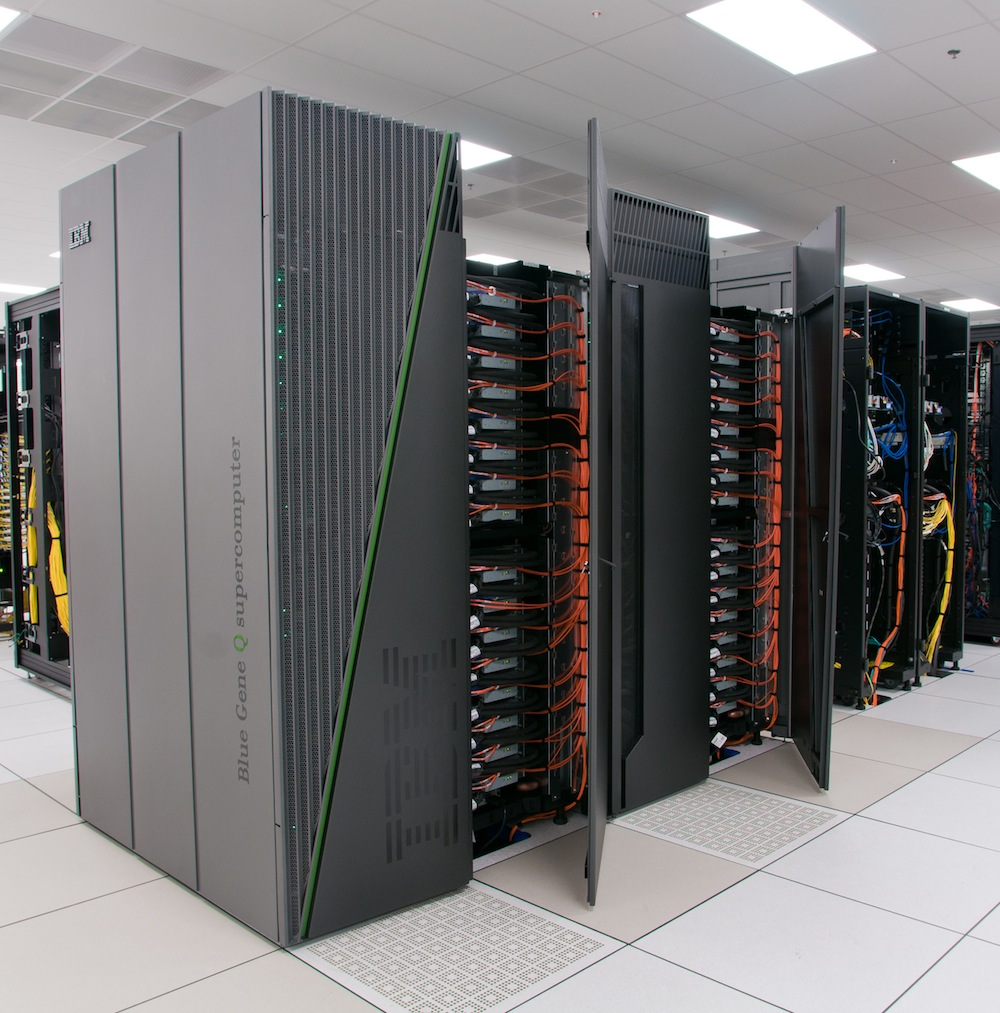
\includegraphics[width=1\textwidth]{figures/mira.jpg}
    \end{column}
  \end{columns}

    \pause
    \begin{block}{Implications}
        \begin{itemize}
            \item Each thread of execution has to:
                \begin{itemize}
                    \item operate on lesser data
                    \item wait relatively longer for remote data
                \end{itemize}
            \item Have to operate in \textbf{strong scaling} regime
            % Even if you don't do anything, an 8GB problem will have to run on
            % more cores a few years from now simply because there will be many
            % more cores for the same 8GB 
            % If a product has to stay ahead of the competition, it has to scale
            % the same problem to even more cores with time to run faster
        \end{itemize}
    \end{block}
\end{frame}


\begin{frame}[t]
\frametitle{Harnessing Parallelism}
\framesubtitle{Trends in System Architecture}
    \begin{itemize}
        \item Growing heterogeneity: Each thread of execution has different abilities
            \begin{itemize}
                \item NUMA cores on each node
                \item Secondary threads in SMT can be less capable (IBM Power 7)
                \item Accelerators (NVIDIA / AMD GPUs, Intel MIC etc)
                \item Some cores run system daemons
                \item Combinations of above
                    \begin{itemize}
                        \item GPUs only on some nodes (BlueWaters: NCSA)
                        \item MIC + SMT nodes (Stampede: TACC)
                    \end{itemize}
            \end{itemize}
        \pause
        \item Each architecture expects different treatment
            \begin{itemize}
                \item GPUs expect evenly divided pieces
                \item SMT might expect uneven pieces (IBM Power7)
            \end{itemize}
    \end{itemize}
    \pause
    \begin{block}{Implications}
        \begin{itemize}
            \item Achieving load balance on such hardware is challenging
            \item Minimizing idle time is extremely difficult
        \end{itemize}
    \end{block}
\end{frame}


\begin{frame}[t]
\frametitle{Harnessing Parallelism}
\framesubtitle{Trends in System Architecture}
  \begin{itemize}
  \item Extracting performance on tighter power / energy budget
  \item Hardware component failures / faults
  \end{itemize}
\end{frame}


\begin{frame}[fragile]
\frametitle{Harnessing Parallelism}
\framesubtitle{Application characteristics}
  \begin{itemize}
  \item Complex physics in multiple, interacting modules
  \item Adaptive, spatial and temporal resolutions
  \item Need for faster solutions (not just larger problems)
  \end{itemize}
\end{frame}


\begin{frame}[t]
\frametitle{Harnessing Parallelism}
\framesubtitle{Programming Models: MPI}
  \begin{itemize}
    \item Highly successful
    \item Universally used
    \item Has supported application evolution from gigascale to petascale
  \end{itemize}
  \begin{itemize}
    \item Library
    \item Communication primitives
  \end{itemize}
\end{frame}


\begin{frame}[fragile]
\frametitle{Harnessing Parallelism}
\framesubtitle{2D Jacobi Iterations: 5-point Stencil}
   \begin{center} 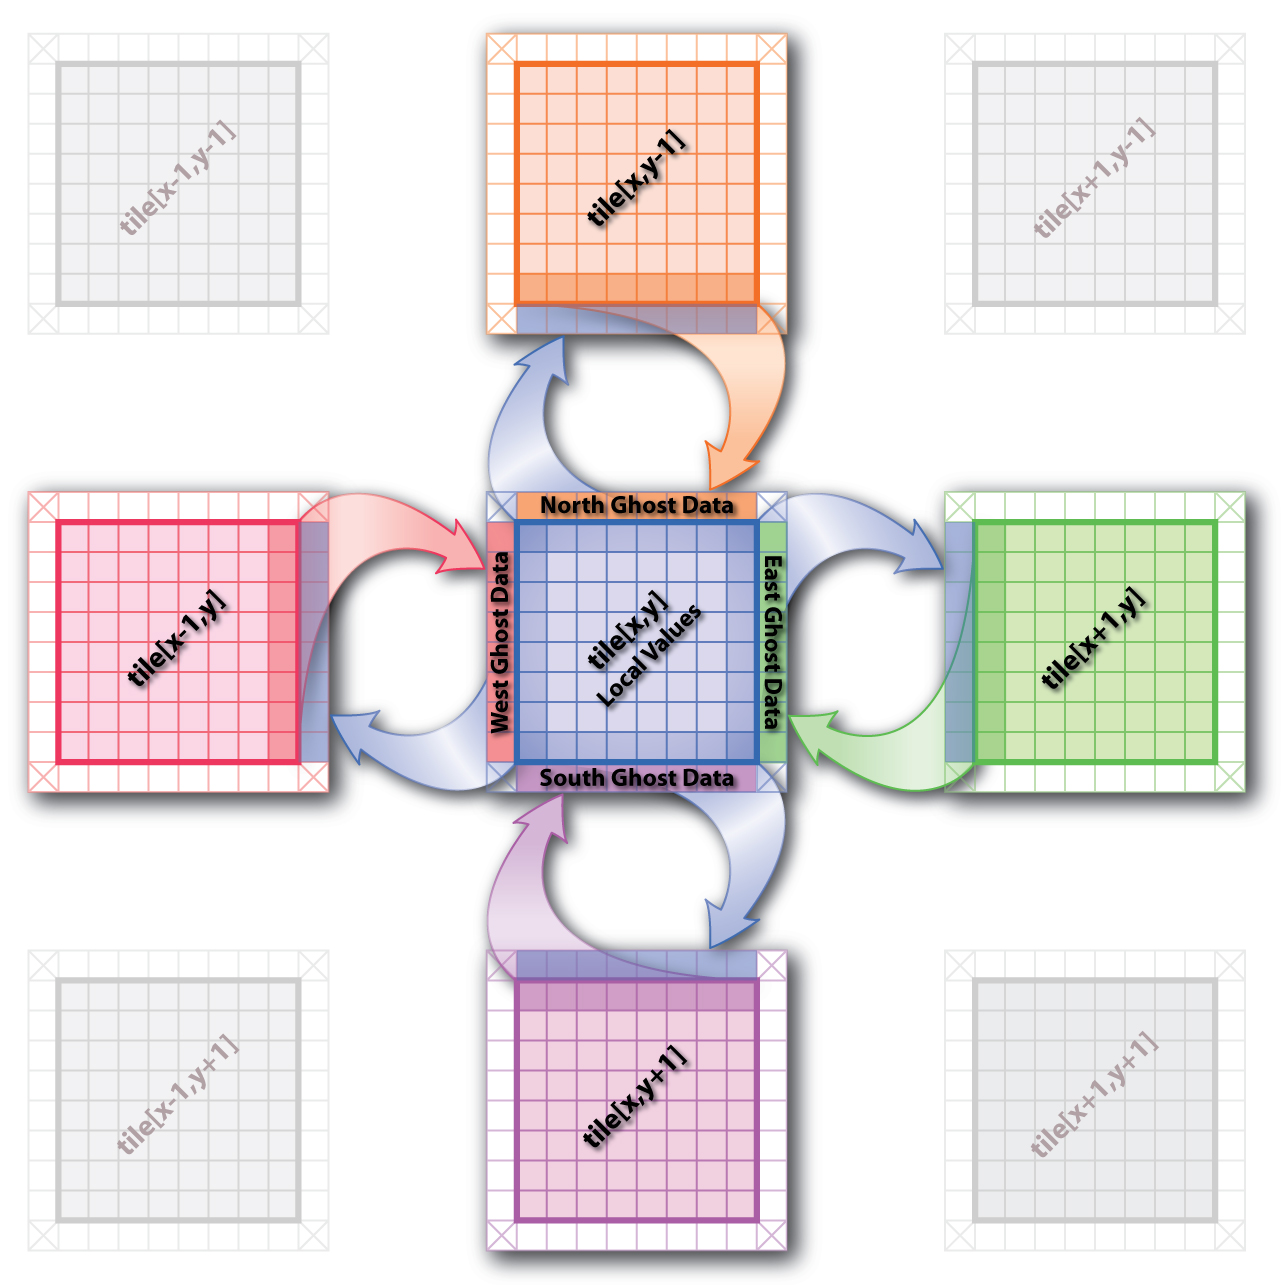
\includegraphics[width=0.6\textwidth]{figures/2DJacobi_NeighborComm.jpg} \end{center}
\end{frame}


\begin{frame}[fragile]
\frametitle{Harnessing Parallelism}
\framesubtitle{2D Jacobi Iterations: No Overlap}
    \lstinputlisting{code/jacobi2D-mpi.c}
\end{frame}


\begin{frame}[fragile]
\frametitle{Harnessing Parallelism}
\framesubtitle{2D Jacobi Iterations: Some Overlap}
    \lstinputlisting{code/jacobi2D-mpi-nonblocking.c}
\end{frame}


\begin{frame}[fragile]
\frametitle{Harnessing Parallelism}
\framesubtitle{Composing Independent Parallel Modules}
    fig to show space division
\end{frame}


\begin{frame}[fragile]
\frametitle{Harnessing Parallelism}
\framesubtitle{Composing Independent Parallel Modules}
    fig to show time division
\end{frame}

\begin{frame}
  \frametitle{Jacobi Reduction}
  \begin{center}
    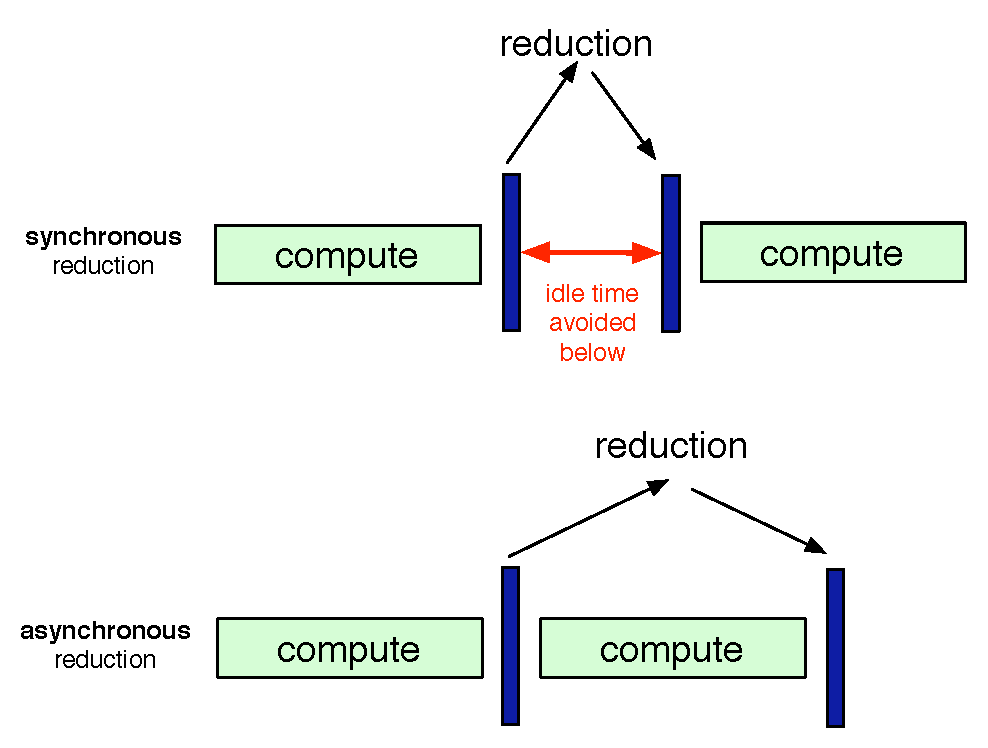
\includegraphics[width=0.8\textwidth]{figures/asyncReduction.pdf}
  \end{center}
\end{frame}
\subsection[Object Design]{Object Design}
\transition{A proven approach: objects}
  \begin{frame}[fragile]
\frametitle{Stuff you already know}
\framesubtitle{Some issues with procedural code}

  \begin{columns}
    \begin{column}{0.4\textwidth}
      \lstinputlisting[basicstyle=\tiny]{code/jacobi2D-mpi.c}
    \end{column}
    \begin{column}{0.6\textwidth}
      \begin{itemize}
      \item Very similar to sequential code
      \item Tied to notion of communicating ranks
      \item Explicitly states order of computation and communication
      \item However no semantic connection between computation and its communication dependencies
      \item Data is not well encapsulated.
      \end{itemize}
    \end{column}
  \end{columns}

\end{frame}


\begin{frame}[shrink]
\frametitle{Stuff you already know}
\framesubtitle{Benefits of Object-based code}
    \begin{itemize}
        \item Objects encapsulate data
        \item Methods represent functionality relevant to that data
        \item Method invocations can modify / update state of the object / data
        \item Computation can be expressed in terms of objects interacting via method invocations
    \end{itemize}
    \begin{block}{}
    \begin{itemize}
        \item Methods are natural units of sequential computation on object data
        \item Thoughtful design yields focused methods with single purpose
        \item Naturally expresses an object's response to inputs (signals / data)
    \end{itemize}
    \end{block}
    \begin{itemize}
        \item Nothing new
        \item Still quite uncommon in HPC code
        \item Its not about language syntax. Its about program structure
    \end{itemize}
}

\transition{A proven approach: method-driven objects}
\begin{frame}[fragile]
  \frametitle{Globally-Visible Objects}
  \begin{center}
    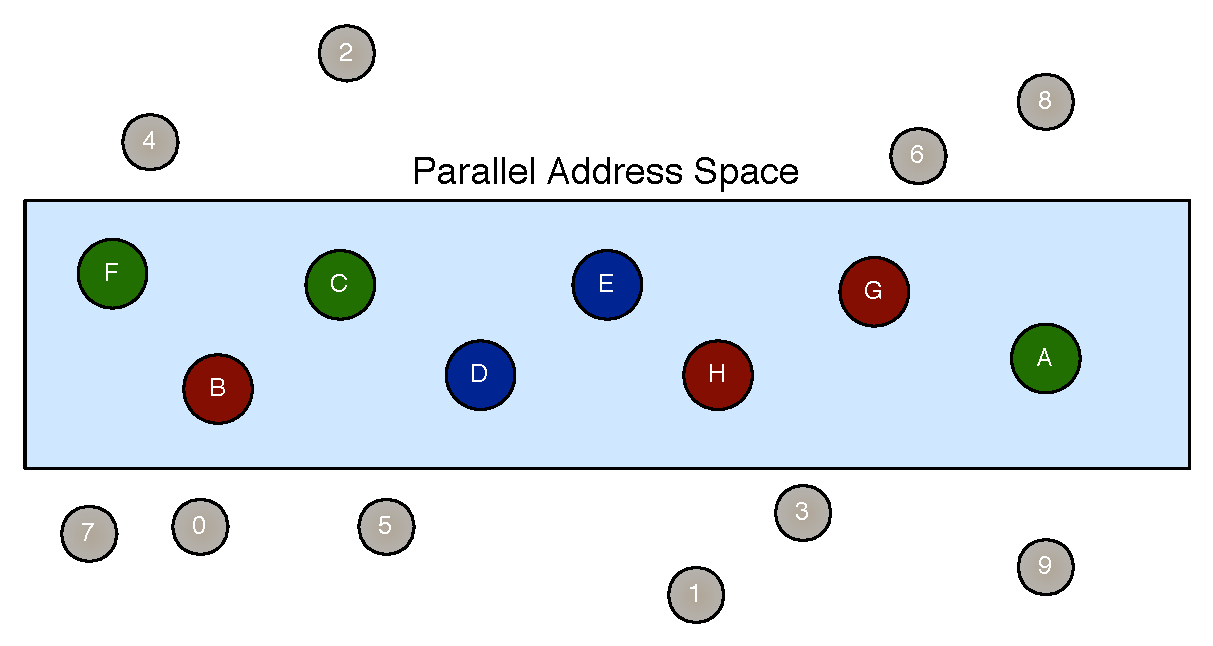
\includegraphics[width=\textwidth]{figures/objectGlobalAddress.pdf}
  \end{center}
  \begin{itemize}
    \item Certain ``selected'' object \emph{instances} are:
      \begin{itemize}
      \item autonomous,
      \item first-class citizens in the parallel address space,
      \item with unique location-independent names
      \end{itemize}
    \item Under the hood, the runtime handles locality and provides the
      mechanisms to promote objects to the parallel space
  \end{itemize}
\end{frame}

\begin{frame}[fragile]
  \frametitle{Globally-Visible Methods}
  \begin{center}
    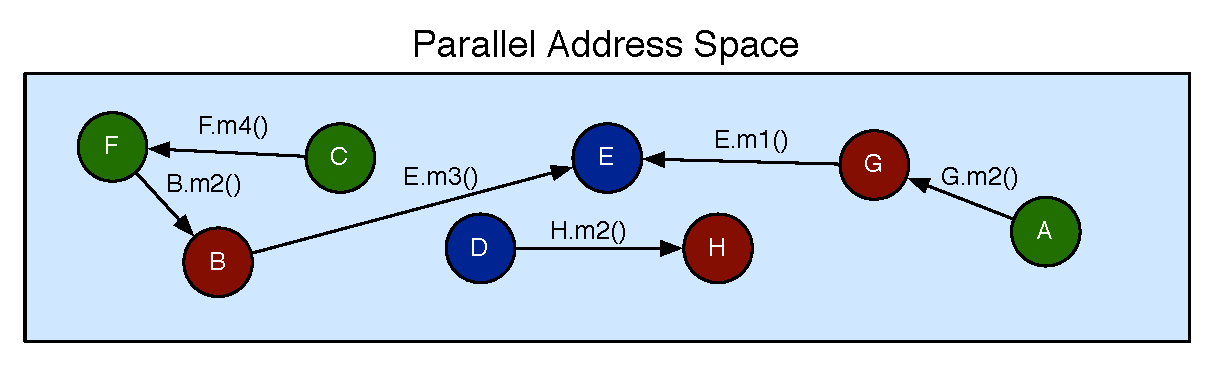
\includegraphics[width=\textwidth]{figures/objectMethodGlobalAddress.pdf}
  \end{center}
  \begin{itemize}
    \item How can objects communicate across address spaces?
      \begin{itemize}
      \item Just like a sequential object-oriented language, a object's
        reference is used to invoke a method
      \item In the parallel space, this is a handle that is transparent of location
      \item A method invocation becomes an act of communication
      \end{itemize}
  \end{itemize}
\end{frame}

\begin{frame}[fragile]
  \frametitle{Method-Driven Asynchronous Communication}
  \begin{center}
    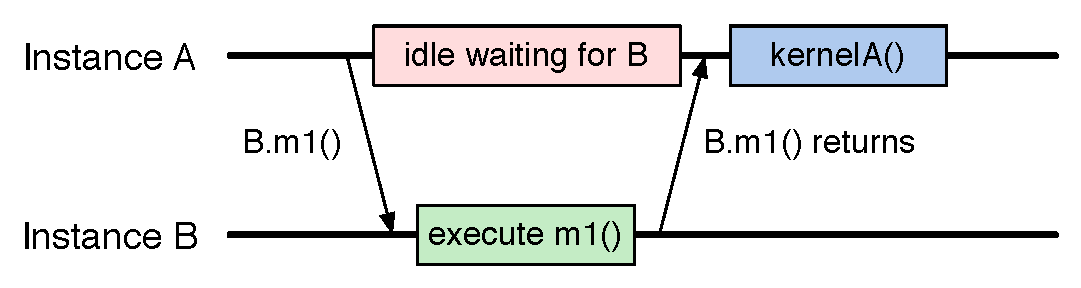
\includegraphics[width=\textwidth]{figures/objectSequence.pdf}
  \end{center}
  \begin{itemize}
  \item What happens if an object waits for a return value from a method
    invocation?
    \begin{itemize}
    \item Performance
    \item Latency
    \item Reasoning about correctness
    \end{itemize}
  \end{itemize}
\end{frame}

\begin{frame}[fragile]
  \frametitle{Design Principle: Do not wait for remote completion}
  \begin{center}
    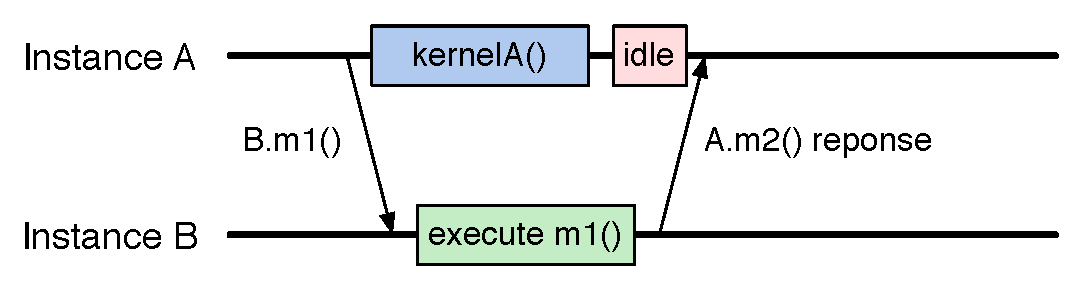
\includegraphics[width=\textwidth]{figures/objectSequenceAsync.pdf}
  \end{center}
  \begin{itemize}
  \item Hence, method invocations should be asynchronous
    \begin{itemize}
    \item No return values
    \end{itemize}
  \item Computations are driven by the incoming data
    \begin{itemize}
    \item Initiated by the sender or method caller
    \end{itemize}
  \end{itemize}
\end{frame}

\begin{frame}
  \frametitle{For example, a Jacobi reduction}
  \begin{center}
    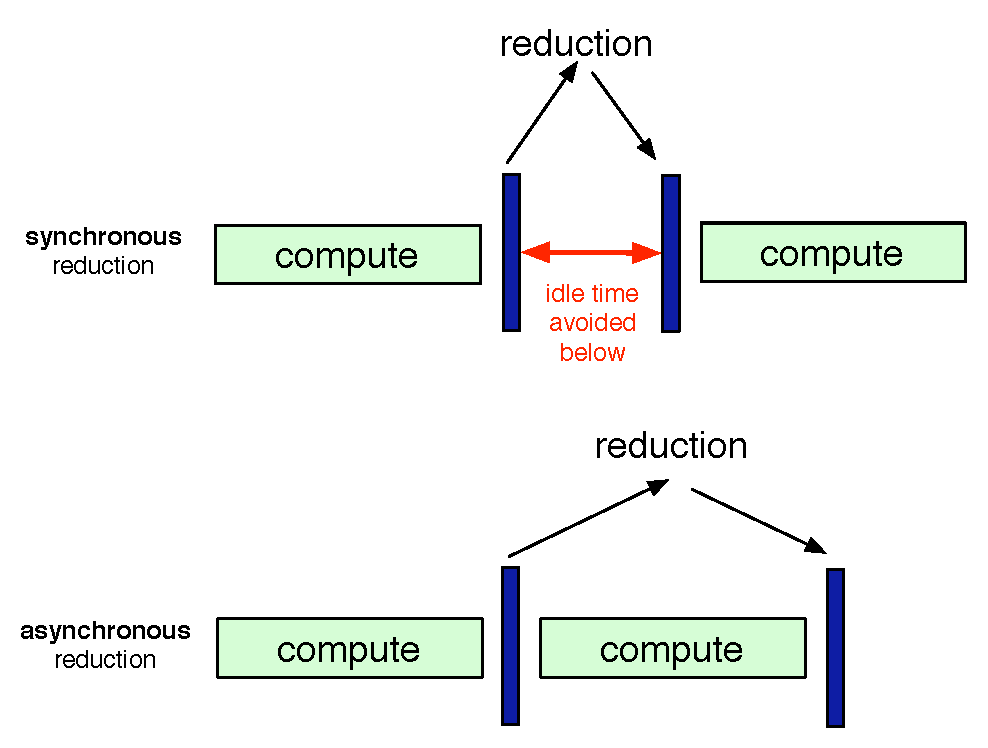
\includegraphics[width=0.8\textwidth]{figures/asyncReduction.pdf}
  \end{center}
\end{frame}

\begin{frame}[fragile]
  \frametitle{Methods: Natural Units of Sequential Computation}
  \begin{columns}
    \begin{column}{0.55\textwidth}
      \begin{itemize}
      \item Methods still have the same sequential semantics
        \begin{itemize}
        \item Atomicity: methods do not execute in parallel
        \end{itemize}
      \item Methods cannot be interrupted  or preempted
      \item Methods interact and update state of an object in the same way
      \item Method sequencing is what changes from sequential computation
      \end{itemize}
    \end{column}
    \begin{column}{0.45\textwidth}
      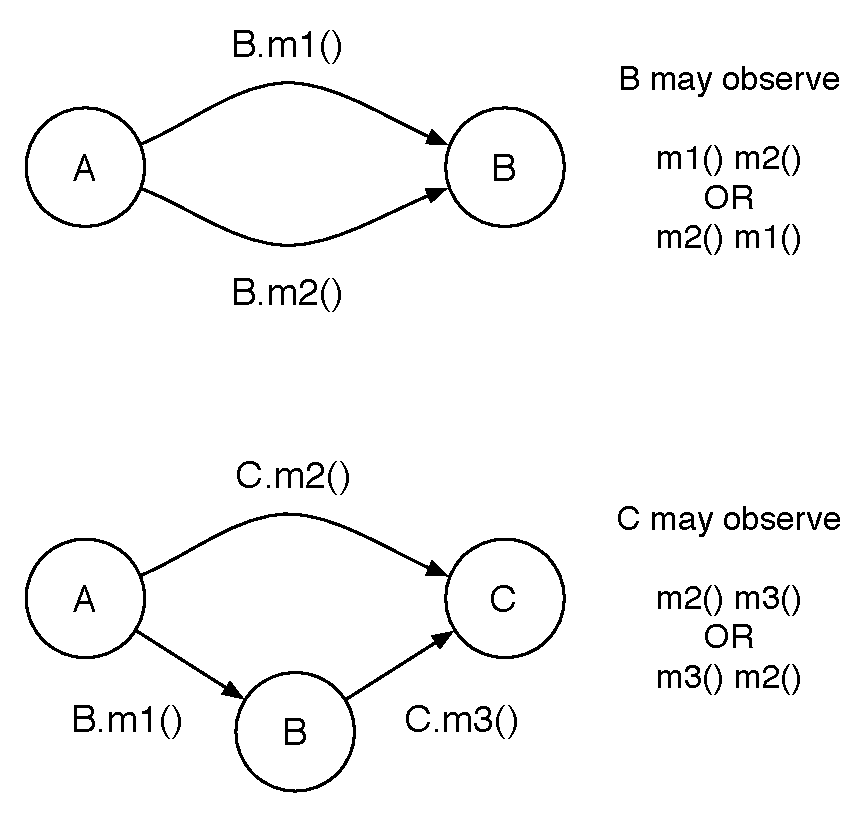
\includegraphics[width=1\textwidth]{figures/sequencing.pdf}
    \end{column}
  \end{columns}
\end{frame}

\begin{frame}[fragile]
  \frametitle{Dependencies and Dataflow}
    \begin{columns}
    \begin{column}{0.55\textwidth}
      \begin{itemize}
      \item A method invocation expresses a dependency in the computation
      \item For example, we can now express a LU decomposition in its natural
        form
        \begin{itemize}
        \item A directed acyclic graph
        \end{itemize}
      \end{itemize}
    \end{column}
    \begin{column}{0.45\textwidth}
      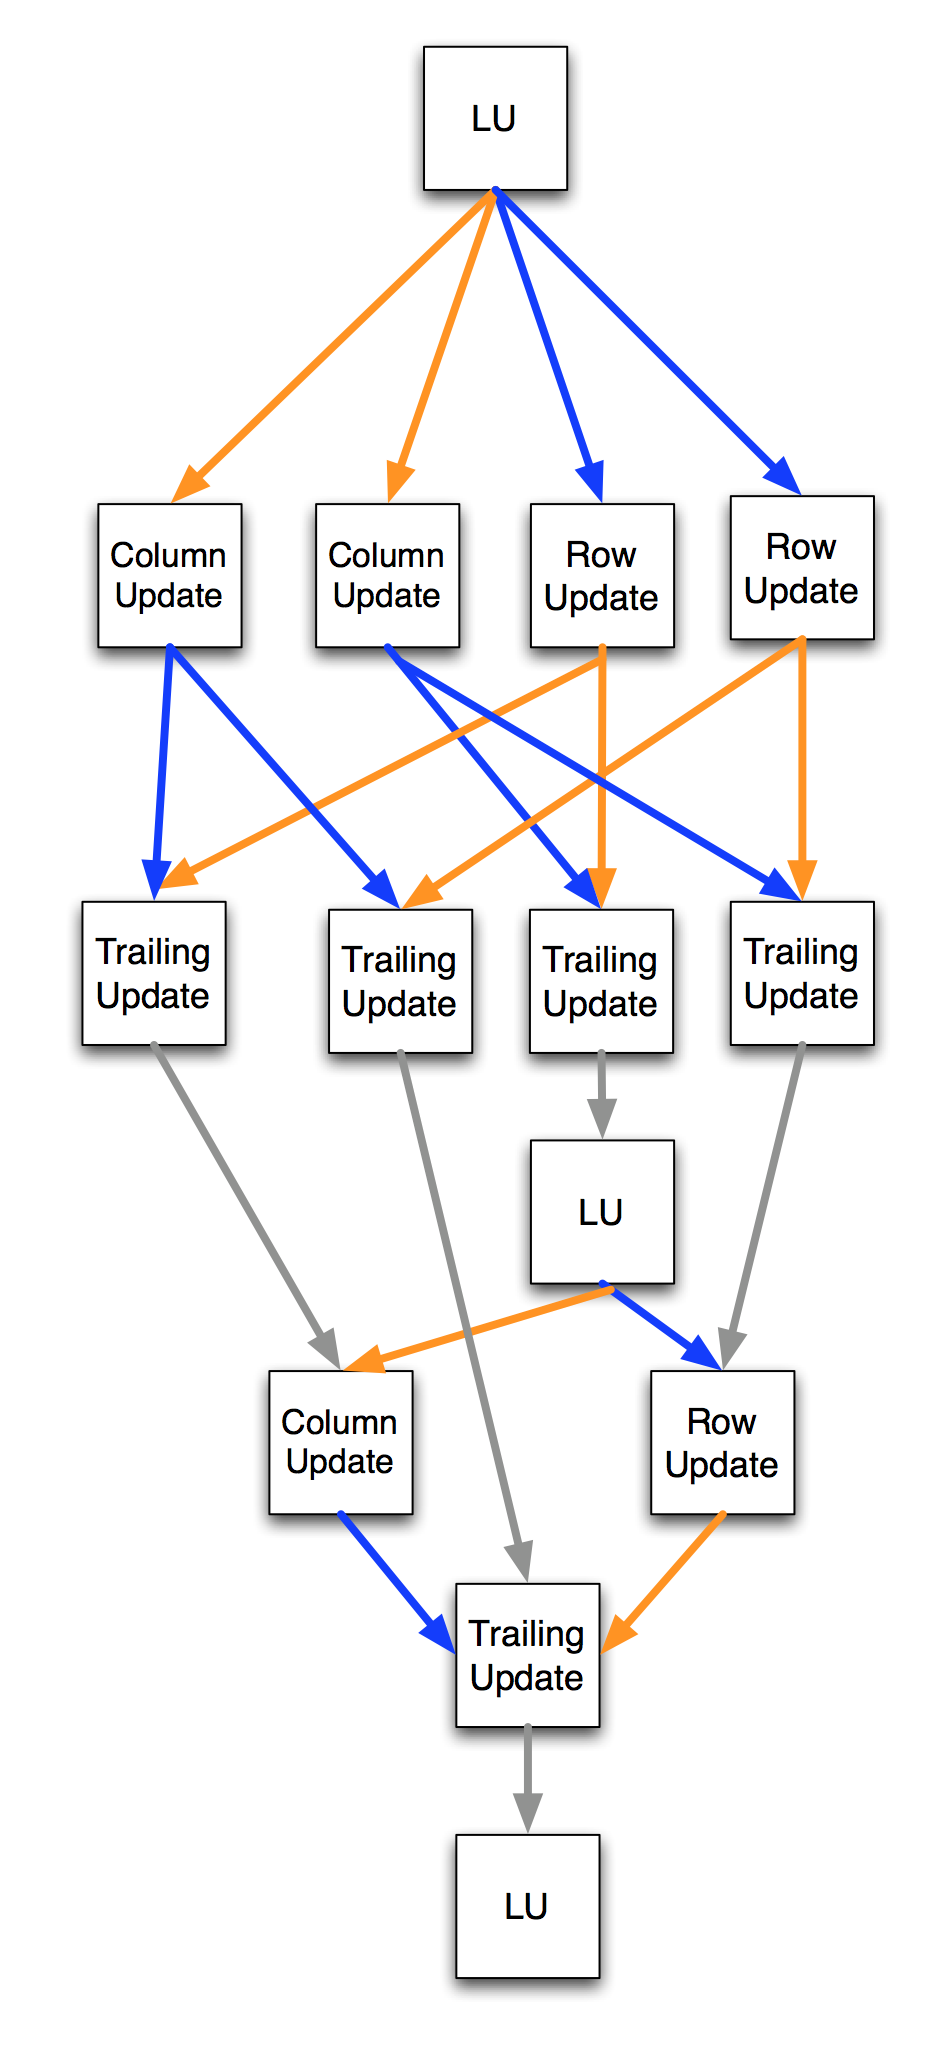
\includegraphics[width=0.7\textwidth]{figures/ludag.png}
    \end{column}
  \end{columns}
\end{frame}
\subsection[Execution Mode]{Execution Model}
\begin{frame}[t]
\frametitle{The Execution Model}
  \begin{itemize}
    \item Several objects live on a single ``processor”
    \begin{itemize}
      \item We will come back what we mean by a processor.
      \begin{itemize}
        \item For now, think of it as a core
      \end{itemize}
    \end{itemize}
  \item As a result, 
    \begin{itemize}
      \item the method invocations directed at objects on that processor will have to be stored in a pool,
      \item And a user-level scheduler will select one invocation from the Quque and and runs it completion
    \end{itemize}
  \end{itemize}
  \begin{center} 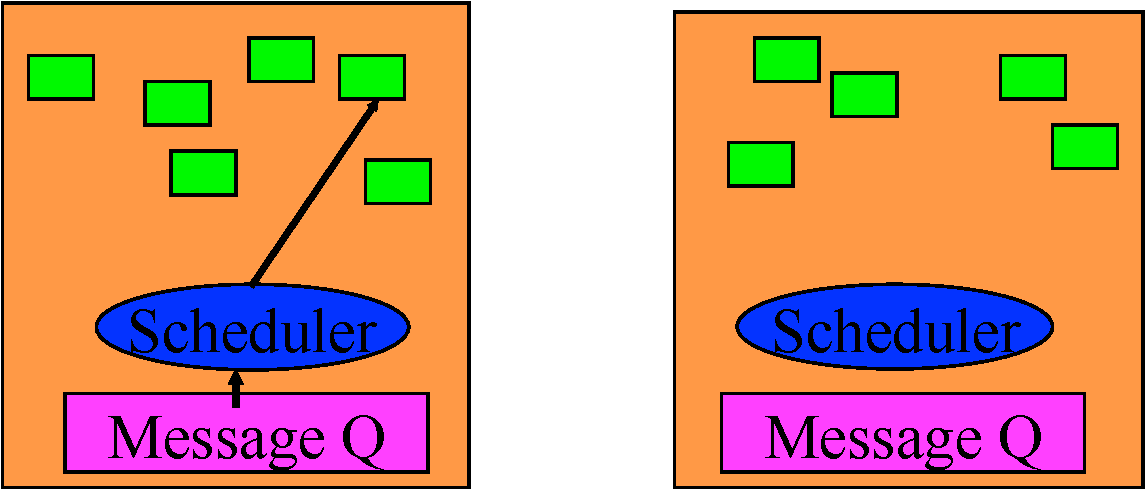
\includegraphics[width=0.7\textwidth]{figures/scheduler} \end{center}
\end{frame}

\begin{frame}[t]
\frametitle{Message-driven Execution}
  \begin{itemize}
    \item Execution is trigggered by availability of a ``message” (a method invocation)
    \item When an entry method executes, 
    \begin{itemize}
      \item it may generate messages for other objects
      \item the RTS deposits them in the message Q on the target processor
    \end{itemize}
  \end{itemize}
  \begin{center} 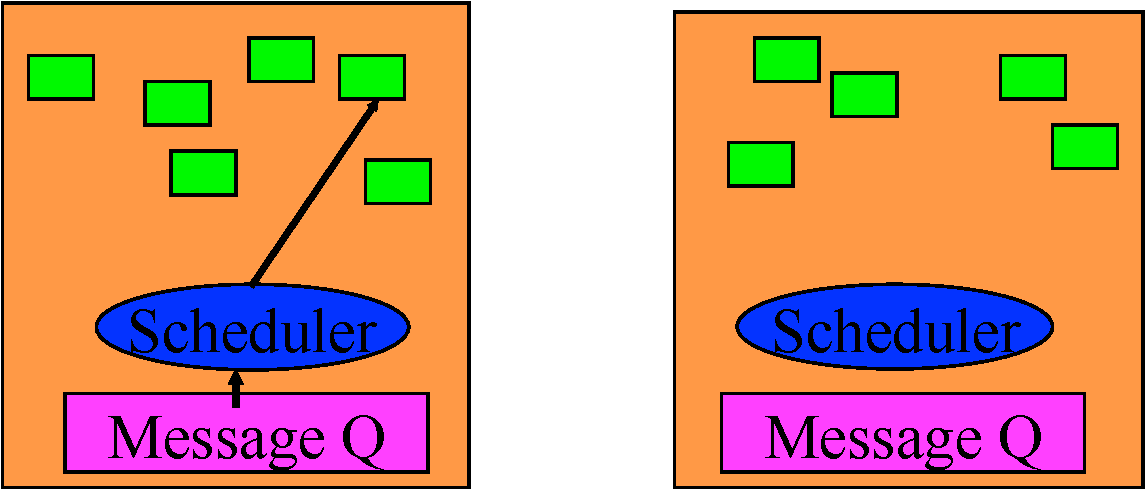
\includegraphics[width=0.7\textwidth]{figures/scheduler} \end{center}
\end{frame}

\begin{frame}[t]
\frametitle{Utility for Multi-cores, Many-cores, Accelerators}
  \begin{itemize}
    \item Objects connote and promote locality
    \item Message-driven execution is
    \begin{itemize}
      \item A strong principle of prediction for data and code use
      \item Much stronger than principle of locality
      \begin{itemize}
        \item Can use to scale memory wall
        \item Prefetching of needed data, e.g, into scratch pad memories
      \end{itemize}
    \end{itemize}
  \end{itemize}
  \begin{center} 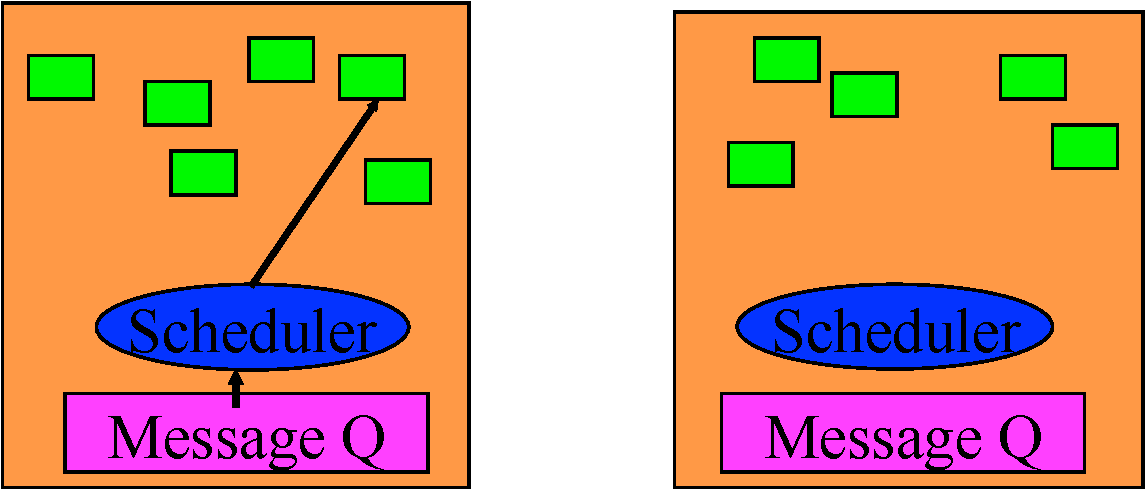
\includegraphics[width=0.7\textwidth]{figures/scheduler} \end{center}
\end{frame}

\begin{frame}[t]
\frametitle{Impact on communication}
  \begin{itemize}
    \item Current use of communication network
    \begin{itemize}
      \item Compute-communicate cycles in typical MPI apps
      \item So, the network is used for a fraction of time
      \item and is on the critical path
    \end{itemize}
    \item So, current communication networks are over-engineered for by necessity
    \item With overdecomposition
    \begin{itemize}
      \item Communication is spread over an iteration
      \item Also, adaptive overlap of communication and computation
    \end{itemize}
  \end{itemize}
\end{frame}

\begin{frame}[t]
\frametitle{Example: Stencil Computation}
  \begin{itemize}
    \item Consider a simple stencil computation
    \begin{itemize}
      \item With traditional design based on traditional methods (e.g.  MPI-based)
      \begin{itemize}
        \item Each processor has a chunk, which alternates between computing and communicating
      \end{itemize}
      \item With Charm++
      \begin{itemize}
        \item Multiple chinks on each processor
        \item Wait time for each chunk overlapped with useful computation for the other
        \item Communication spreads over time
      \end{itemize}
      \item \textcolor{red}{A Simple schematic timeline for both approaches?}
    \end{itemize}
  \end{itemize}
\end{frame}

\begin{frame}[t]
\frametitle{Example: Stencil Computation}
  \begin{center} 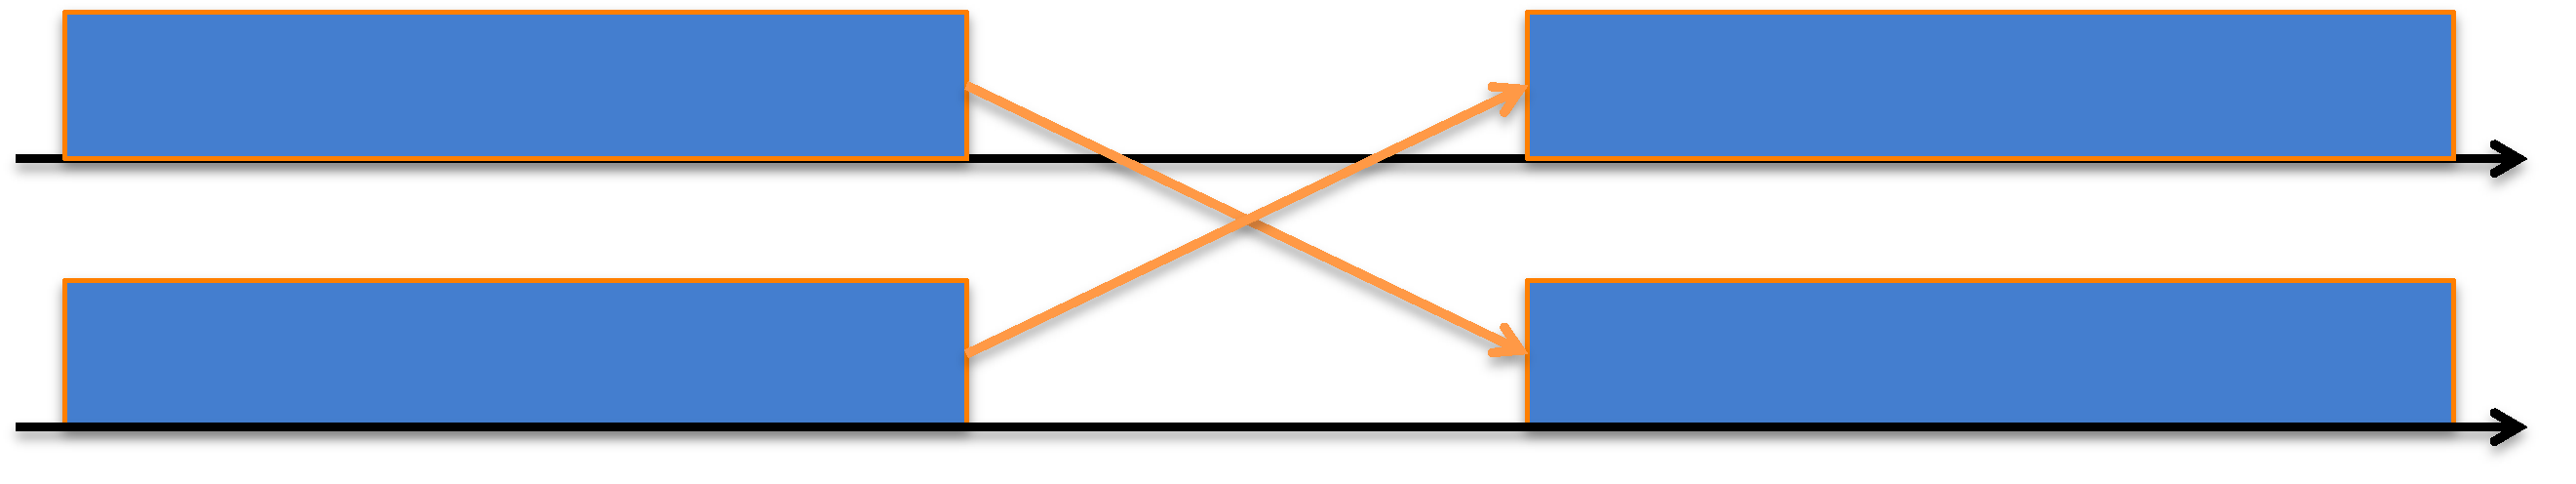
\includegraphics[width=\textwidth]{figures/stencil_timeline} \end{center}
\end{frame}

\begin{frame}[t]
\frametitle{Example: Stencil Computation}
Without message-driven execution (and virtualization), you get either: Space-division

  \begin{center} 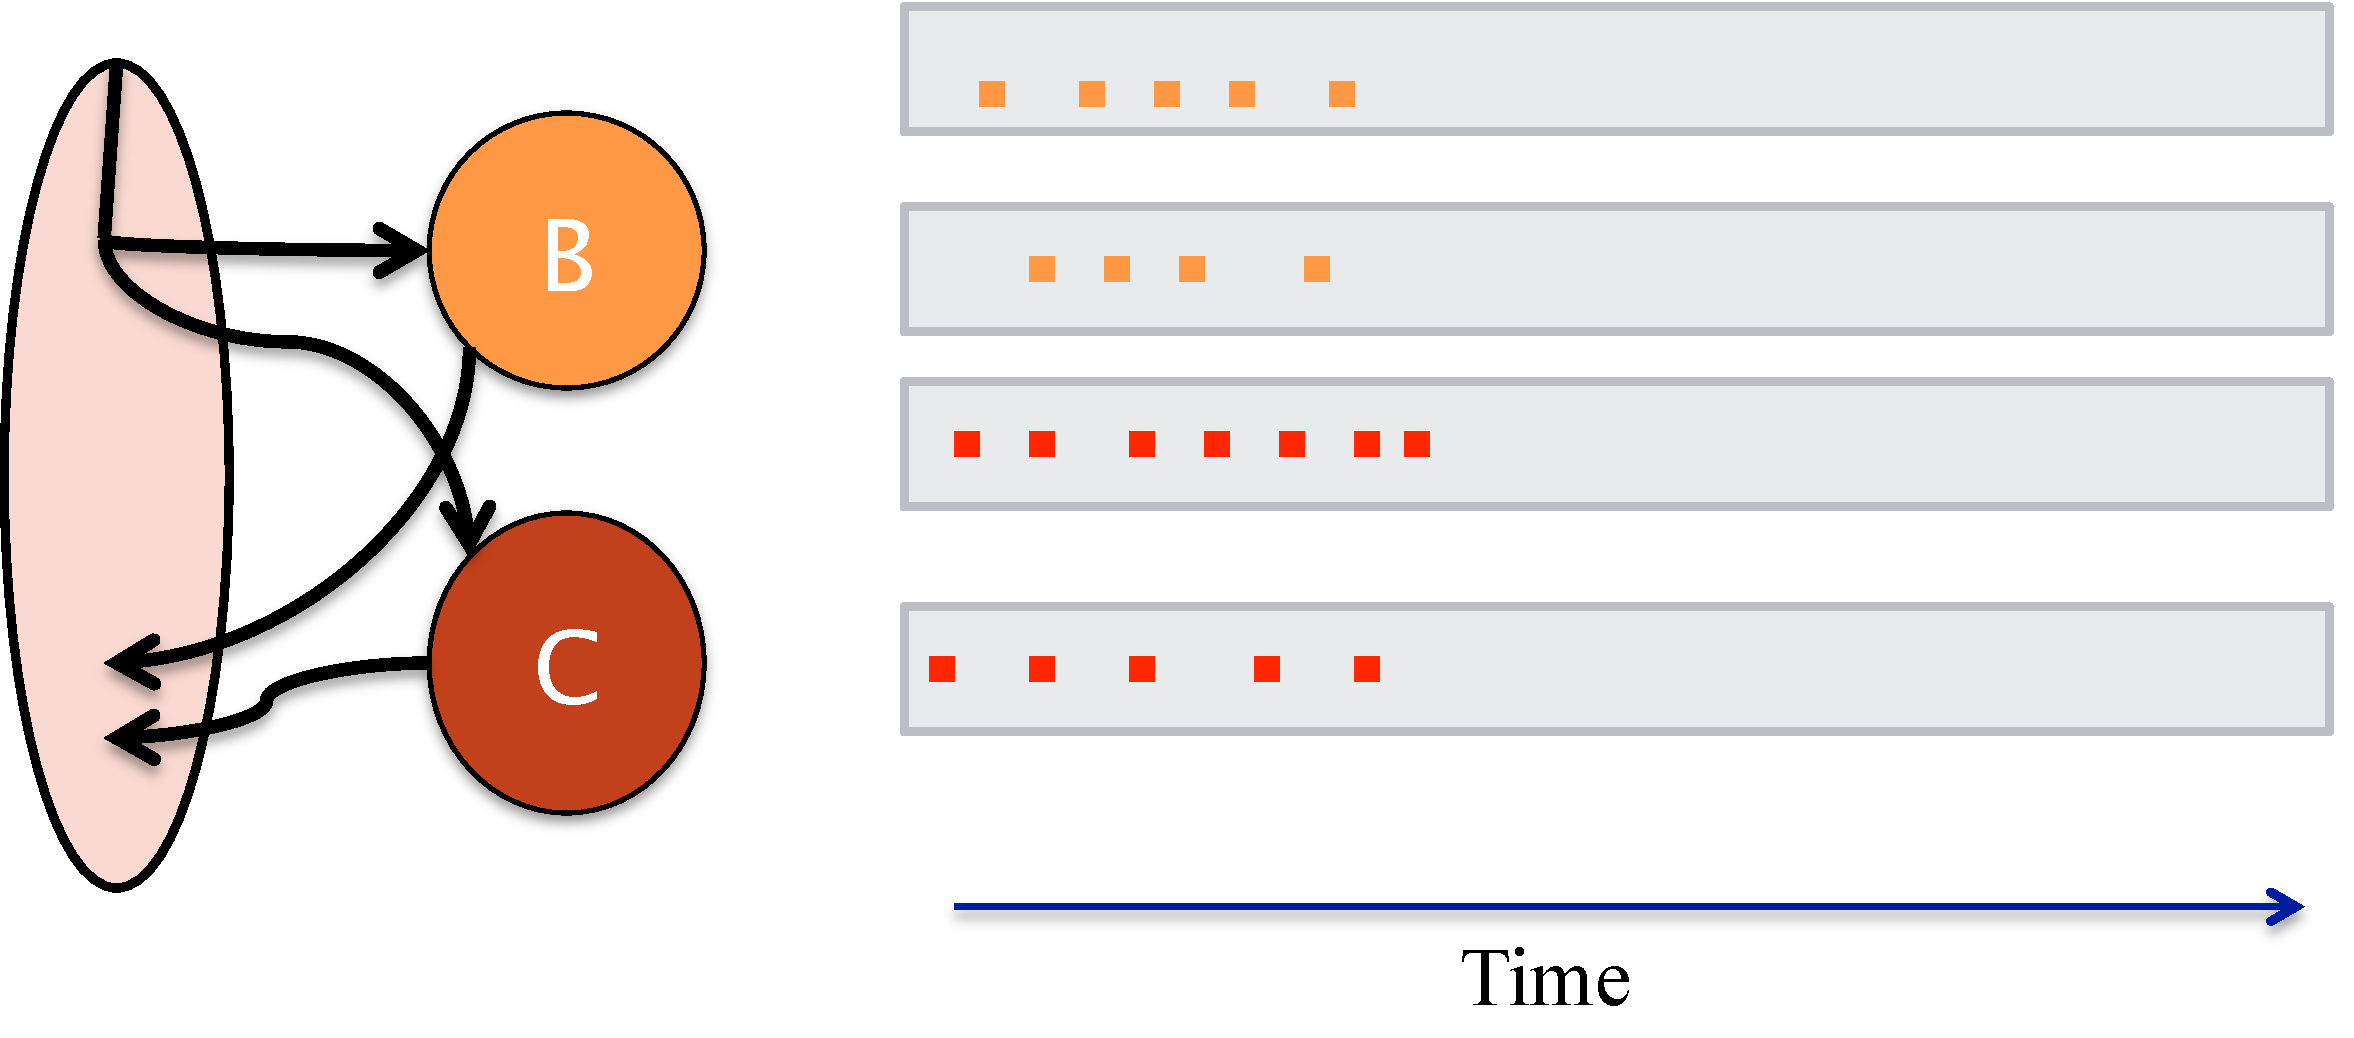
\includegraphics[width=\textwidth]{figures/stencil_space} \end{center}
\end{frame}

\begin{frame}[t]
\frametitle{Example: Stencil Computation}
Sequentialization

  \begin{center} 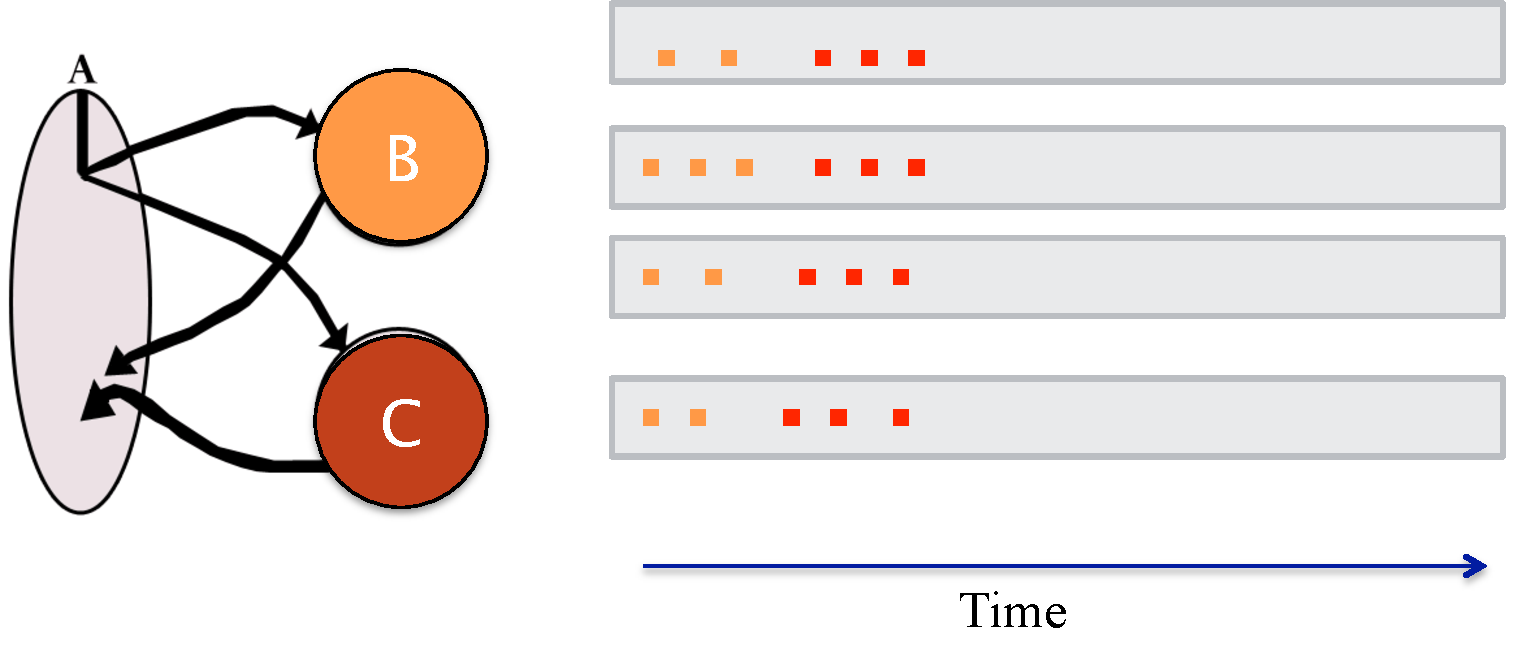
\includegraphics[width=\textwidth]{figures/stencil_seq} \end{center}
\end{frame}

\begin{frame}[t]
\frametitle{Example: Stencil Computation}
Powerpoints defeats Latex - dont know how to recreate the catchy animation from
original slides
\end{frame}

\begin{frame}[t]
\frametitle{MD Parallelization Using Charm++}
The computation is decomposed into ``natural” objects of the application, which
are assigned to processors by Charm++ RTS
  \begin{center} 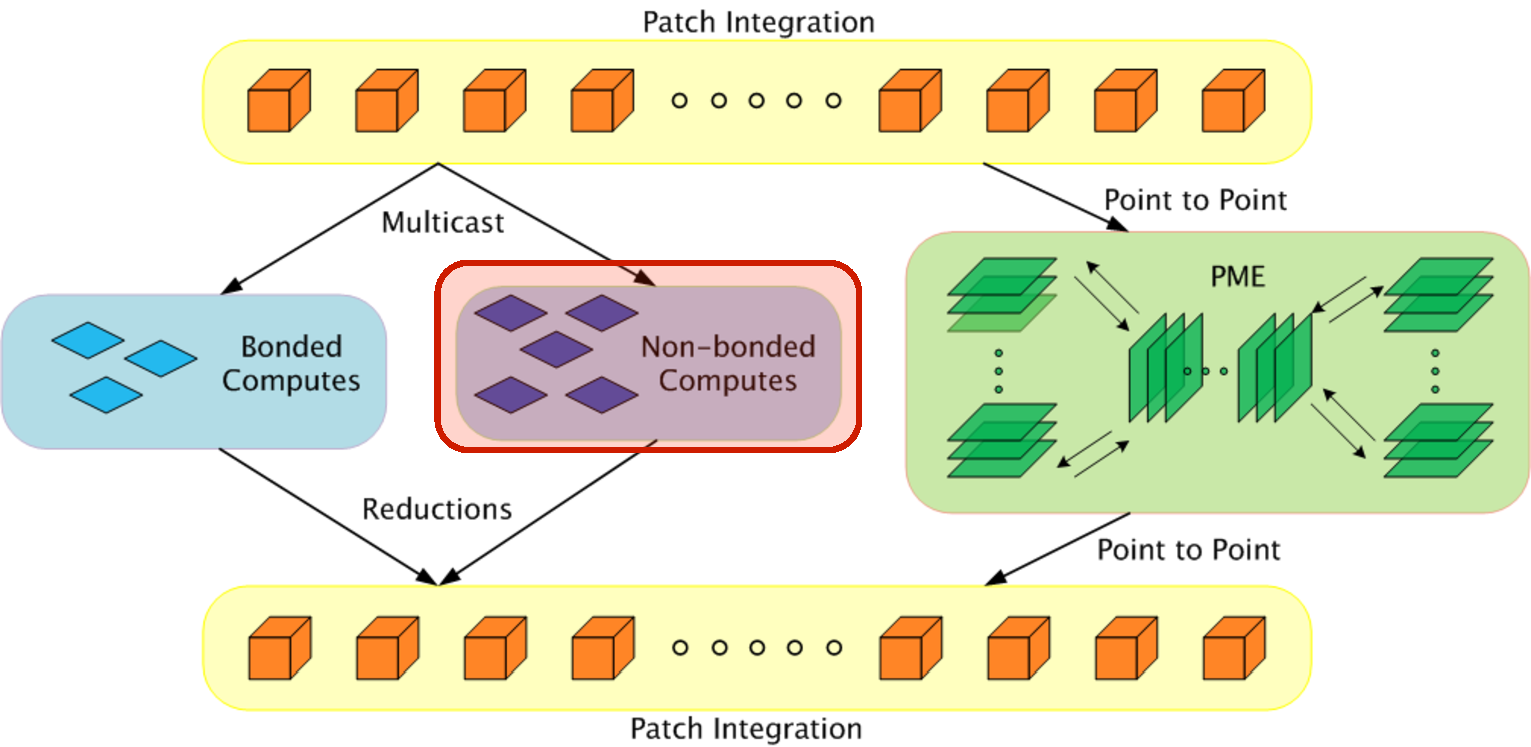
\includegraphics[width=\textwidth]{figures/md_parallelize.pdf} \end{center}
\end{frame}

\begin{frame}[t]
\frametitle{Decomposition Independent of numCores}
  \begin{columns}
    \column{.7\textwidth}
    \begin{itemize}
      \item Rocket simulation under traditional MPI
    \end{itemize}
    \begin{center} 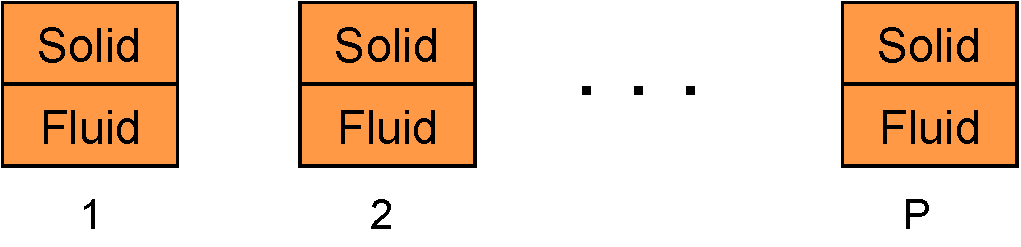
\includegraphics[width=.6\textwidth]{figures/rocket_mpi} \end{center}
    \pause
    \begin{itemize}
      \item Rocket simulation with migratable objects
    \end{itemize}
    \begin{center} 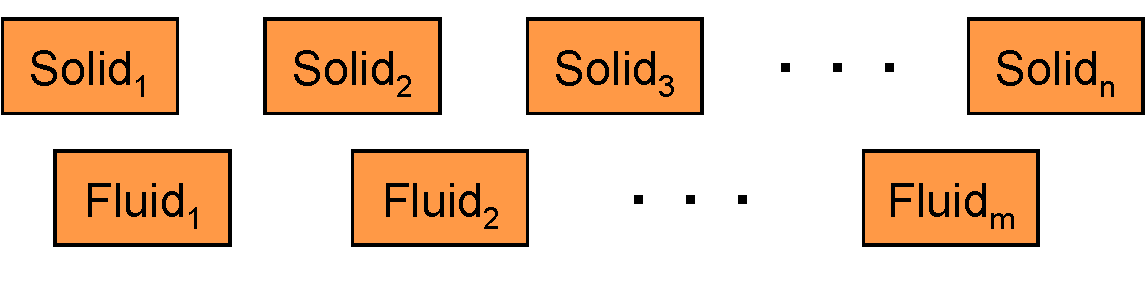
\includegraphics[width=.6\textwidth]{figures/rocket_charm} \end{center}
    \begin{itemize}
      \item
      \begin{itemize}
      \item Benefit: load balance, communication optimizations, modularity
      \end{itemize}
    \end{itemize}
    \column{.3\textwidth}
    \vfill
    \visible<1->{
    \begin{center} \includegraphics<0->[width=\textwidth]{figures/rocket.png} \end{center}
    }
    \vfill
  \end{columns}
\end{frame}

\begin{frame}[t]
\frametitle{Migratability}
  \begin{itemize}
    \item Once the programmer has written the code without reference to processors
      \begin{itemize}
        \item With all the communication expressed as that between objects
      \end{itemize}
    \item The system is free to migrate the objects across processors as and when it pleases
      \begin{itemize}
        \item It must ensure it can deliver method invocations to the objects, whereever they go
        \item This migratability turns out to be a key attribute for empowering an adaptive runtime system
      \end{itemize}
  \end{itemize}
\end{frame}





\subsection[Benefits]{Benefits of Charm++}
\begin{frame}[fragile]
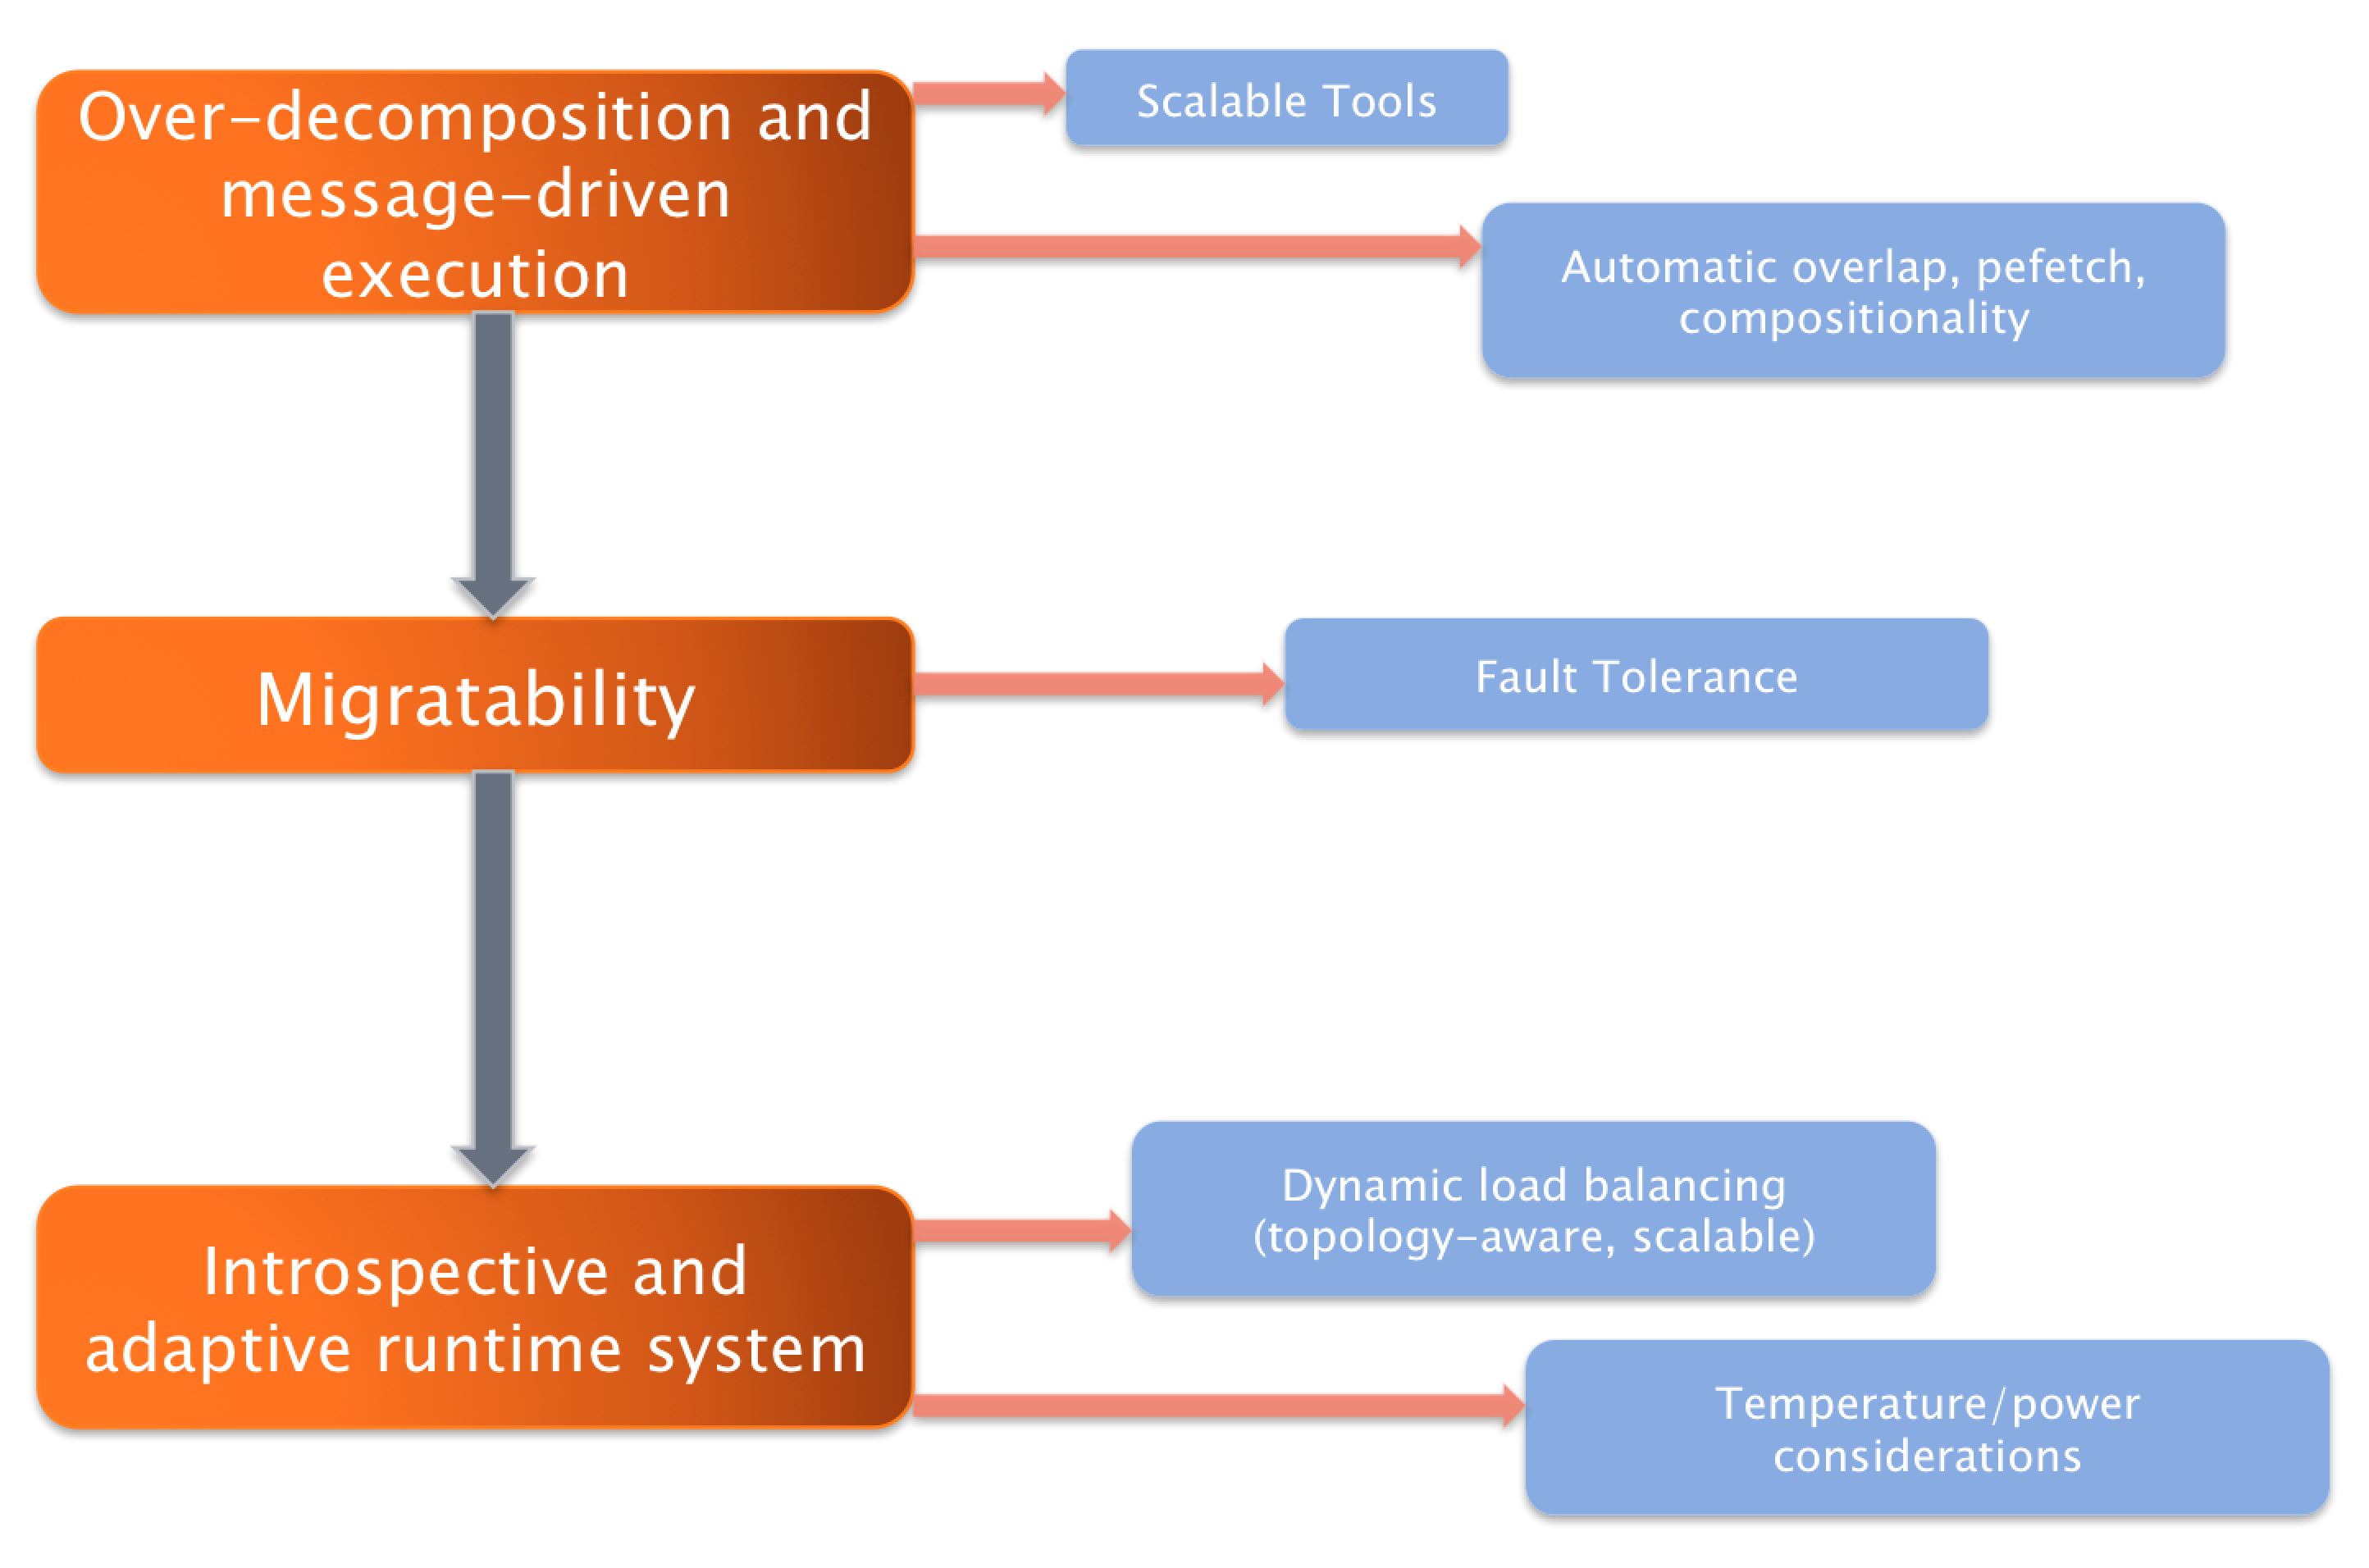
\includegraphics[width=0.9\textwidth]{figures/charmOutline.png}
\end{frame}

\begin{frame}[fragile]
\frametitle{Load Balancing}
\begin{itemize}
 \item Static
   \begin{itemize}
   \item Irregular applications
   \item Programmer shouldn't have to figure out ideal mapping
   \end{itemize}
 \item Dynamic
   \begin{itemize}
   \item Applications are increasingly using adaptive strategies
   \item Abrupt refinements
   \item Continuous migration of work: e.g. particles in MD
   \end{itemize}
 \item Challenges
   \begin{itemize}
   \item Performance limited by most overloaded processor
   \item The chance that one processor is severely overloaded gets higher as
     \#processors increases
   \end{itemize}
\end{itemize}
\begin{center}\textbf{Migratable Objects Empower Automated Load Balancing!}\end{center}
\end{frame}


\begin{frame}[fragile]
\frametitle{Principle of Persistence}
\begin{itemize}
 \item Once the computation is expressed in terms of its natural (migratable)
   objects
 \item Computational loads and communication patterns \emph{tend to} persist,
   even in dynamic computations
 \item So, recent past is a good predictor of near future
 \item The runtime system mediates communication between objects, and schedules
   execution of objects, so it can introspect: record computation loads and
   communication graphs
\end{itemize}
\end{frame}


\begin{frame}[fragile]
\frametitle{A quick Example}
\framesubtitle{Weather Forecasting in BRAMS}
\begin{itemize}
 \item Brams: Brazillian weather code (based on RAMS)
 \item AMPI version (Eduardo Rodrigues, with Mendes and J. Panetta)
\end{itemize}
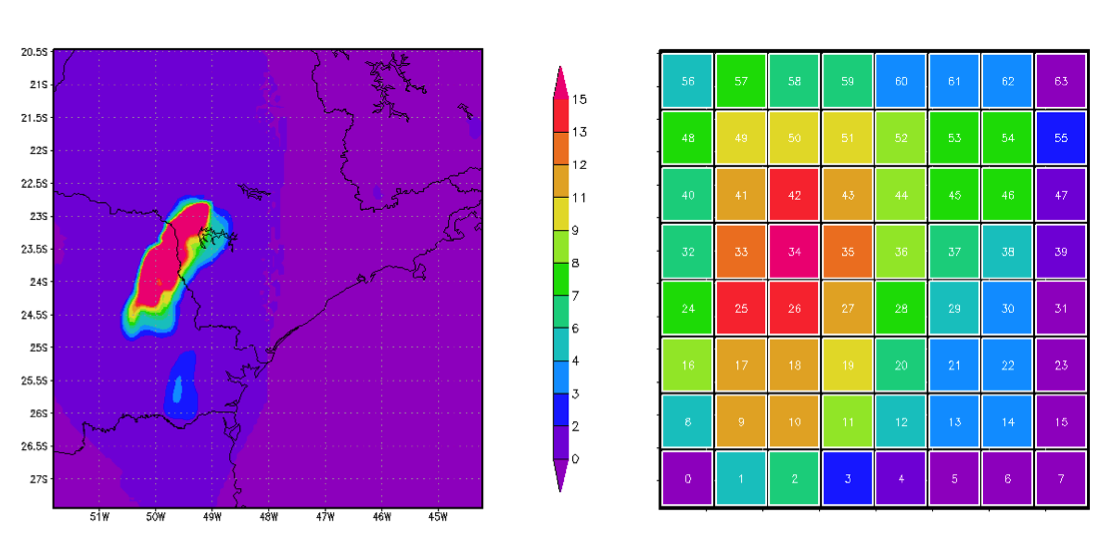
\includegraphics[width=0.9\textwidth]{figures/bramsVisual.png}
\end{frame}


\begin{frame}[fragile]
\frametitle{Basic Virtualization of BRAMS}
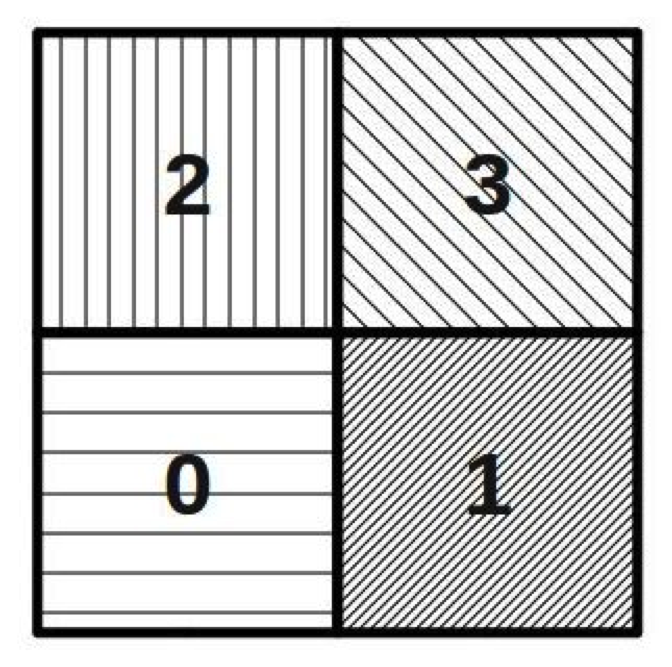
\includegraphics[width=0.5\textwidth]{figures/bramsNonVirtual.png}%
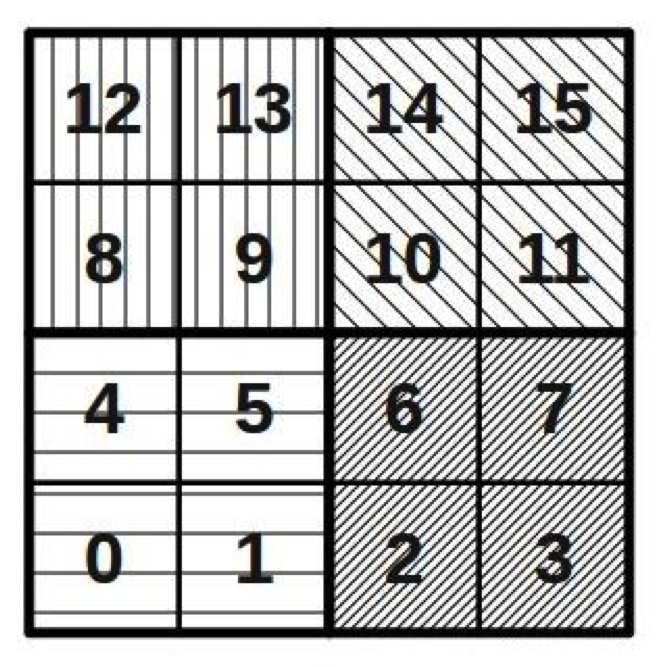
\includegraphics[width=0.5\textwidth]{figures/bramsVirtual.png}
\end{frame}

\begin{frame}[fragile]
\frametitle{Baseline: 64 objects on 64 processors}
\begin{center}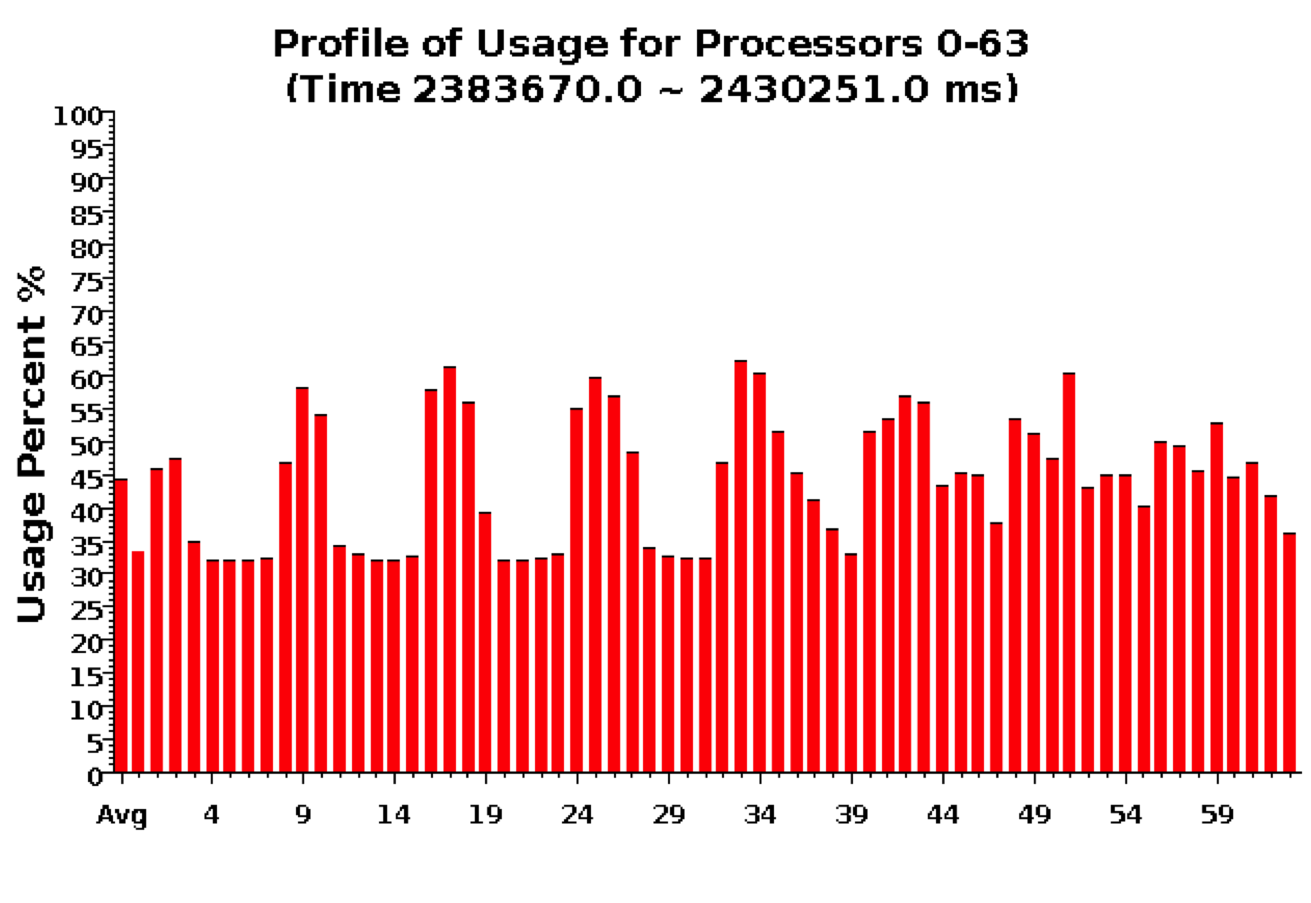
\includegraphics[width=0.9\textwidth]{figures/usageNonVirtual.png}\end{center}
\end{frame}

\begin{frame}[fragile]
\frametitle{Over-decomposition: 1024 objects on 64 processors}
\framesubtitle{Benefits from communication/computation overlap}
\begin{center}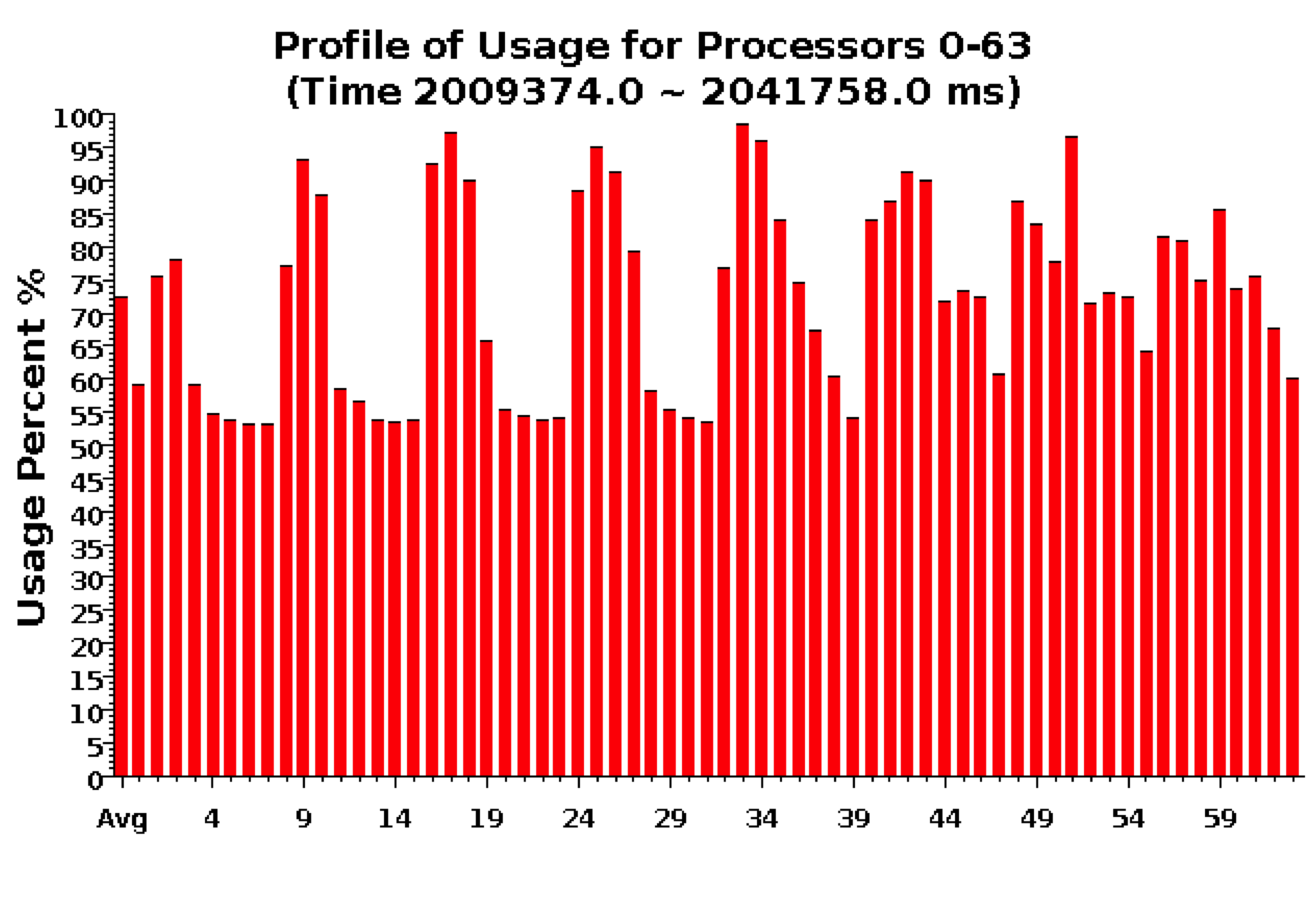
\includegraphics[width=0.9\textwidth]{figures/usageVirtual.png}\end{center}
\end{frame}

\begin{frame}[fragile]
\frametitle{With Load Balancing: 1024 objects on 64 processors}
\begin{center}
\begin{itemize}
\item No overdecomp (64 threads): 4988 sec
\item Overdecomp into 1024 threads: 3713 sec
\item Load balancing (1024 threads): 3367 sec
\end{itemize}
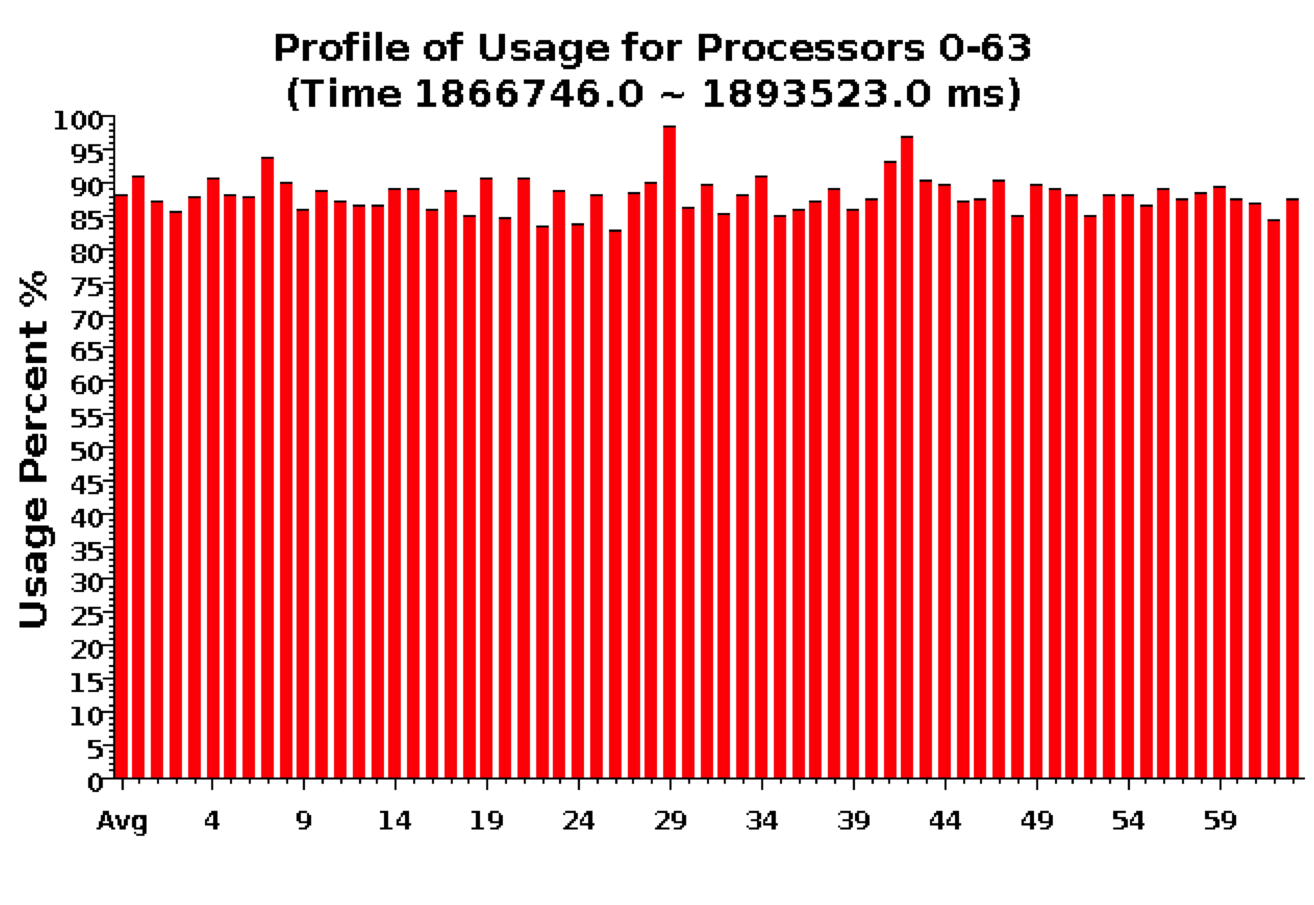
\includegraphics[width=0.8\textwidth]{figures/usageLB.png}
\end{center}
\end{frame}

\subsection[Collections]{Object Collections}

% TODO: add picture of collections
\begin{frame}[fragile]
  \frametitle{Collections of Objects}
  \begin{itemize}
    \item Many problems have inherent order or structure
    \item Especially traditional `technical computing' problems
    \item Solution should use matching abstractions
    \item Arrays, lists, maps of parallel objects
    \item Specific segment of data, and associated computation and
      communication
    \item Need system support for efficient indexing
  \end{itemize}
\end{frame}

\begin{frame}[fragile]
  \frametitle{Collections of Objects: Concepts}
  \begin{itemize}
    \item Basic examples
      \begin{itemize}
      \item Matrix block
      \item Chunk of unstructured mesh
      \item Portion of distributed data structure
      \item Volume of simulation space
      \end{itemize}
      \pause
    \item Advanced Examples
      \begin{itemize}
      \item Abstract portions of computation
      \item Interactions among basic objects or underlying entities
      \end{itemize}
  \end{itemize}
\end{frame}

\begin{frame}[fragile]
  \frametitle{Collections of Objects}
  \begin{itemize}
    \item Structured: 1D, 2D, \ldots, 6D
    \item Unstructured: Anything hashable
      \pause
    \item Dense
    \item Sparse
      \pause
    \item Static - all created at once
    \item Dynamic - elements come and go
  \end{itemize}
\end{frame}

\begin{frame}[fragile]
  \frametitle{Collections of Objects: Communication}
  \begin{itemize}
    \item Point-to-point: to one element of a collection
    \item Broadcast: message to whole collection
    \item Multicast: message to subset of collection
    \item Reductions: message from (part of) collection
    \item Runtime system must provide efficient delivery for all
  \end{itemize}
\end{frame}

\begin{frame}[fragile]
  \frametitle{Collections of Objects: Runtime Service}
  \begin{itemize}
    \item System knows how to `find' objects efficiently: $(collection, index) \to processor$
    \item Applications can specify a mapping, or use simple
      runtime-provided options (e.g. blocked, round-robin)
    \item Distribution can be static, or dynamic!
    \item Key abstraction: application logic doesn't change, even
      though performance might
  \end{itemize}
\end{frame}

\begin{frame}[fragile]
  \frametitle{Collections of Objects: Runtime Service}
  \begin{itemize}
    \item Can develop and test logic in objects separately from their distribution
    \item Separation in time: make it work, then make it fast
    \item Division of labor: domain specialist writes object code, computationalist writes mapping
    \item Portability: different mappings for different systems, scales, or configurations
    \item Shared progress: improved mapping techniaues can benefit existing code
  \end{itemize}
\end{frame}




%% Object Collections: Supporting Data Decomposition (Phil)

%%     Motivate why object collections are needed
%%         simple adding numbers example
%%     Object Collections
%%         decompose data and associated work
%%         1/2/3D or more (eg: mesh chunk)
%%         dense / sparse (sparse solvers, collision detection)
%%         grow / shrink dynamically (AMR)
%%         each object exposes same functionality (methods)
%%         collection should be collectively addressable (method invocation on all objects)
%%         show sample pseudo-code snippets
%%     Object Collections: Collectives
%%     Examples
%%         simple scale a distributed vector (mcast)
%%         simple add array of numbers (mcast + redn)
%%         matrix vector product (mcast + gather)

\subsection[ChaNGa Design]{ChaNGa Design}
\transition{ChaNGa Design}
\begin{frame}[t]
\frametitle{Molecular Dynamics in NAMD}
  \begin{columns}
  \column{.8\textwidth}
  \begin{itemize}
    \item Collection of charged atoms, with bonds
    \begin{itemize}
      \item Newtonian mechanics
      \item Relatively small of atoms (100K – 10M)
    \end{itemize}
    \pause
    \item Calculate forces on each atom 
    \begin{itemize}
      \item Bonds
      \item Non-bonded: electrostatic and van der Waal’s
      \begin{itemize}
        \item Short-distance: every timestep
        \item Long-distance: using PME (3D FFT)
        \item Multiple Time Stepping : PME every 4 timesteps 
      \end{itemize}
    \end{itemize}
    \pause
    \item Calculate velocities and advance positions
    \item Challenge: femtosecond time-step, millions needed!
  \end{itemize}
  \pause
  \textcolor{red}{Collaboration with K. Schulten, R. Skeel, and coworkers}
  \column{.2\textwidth}
  \vfill
  \begin{center} 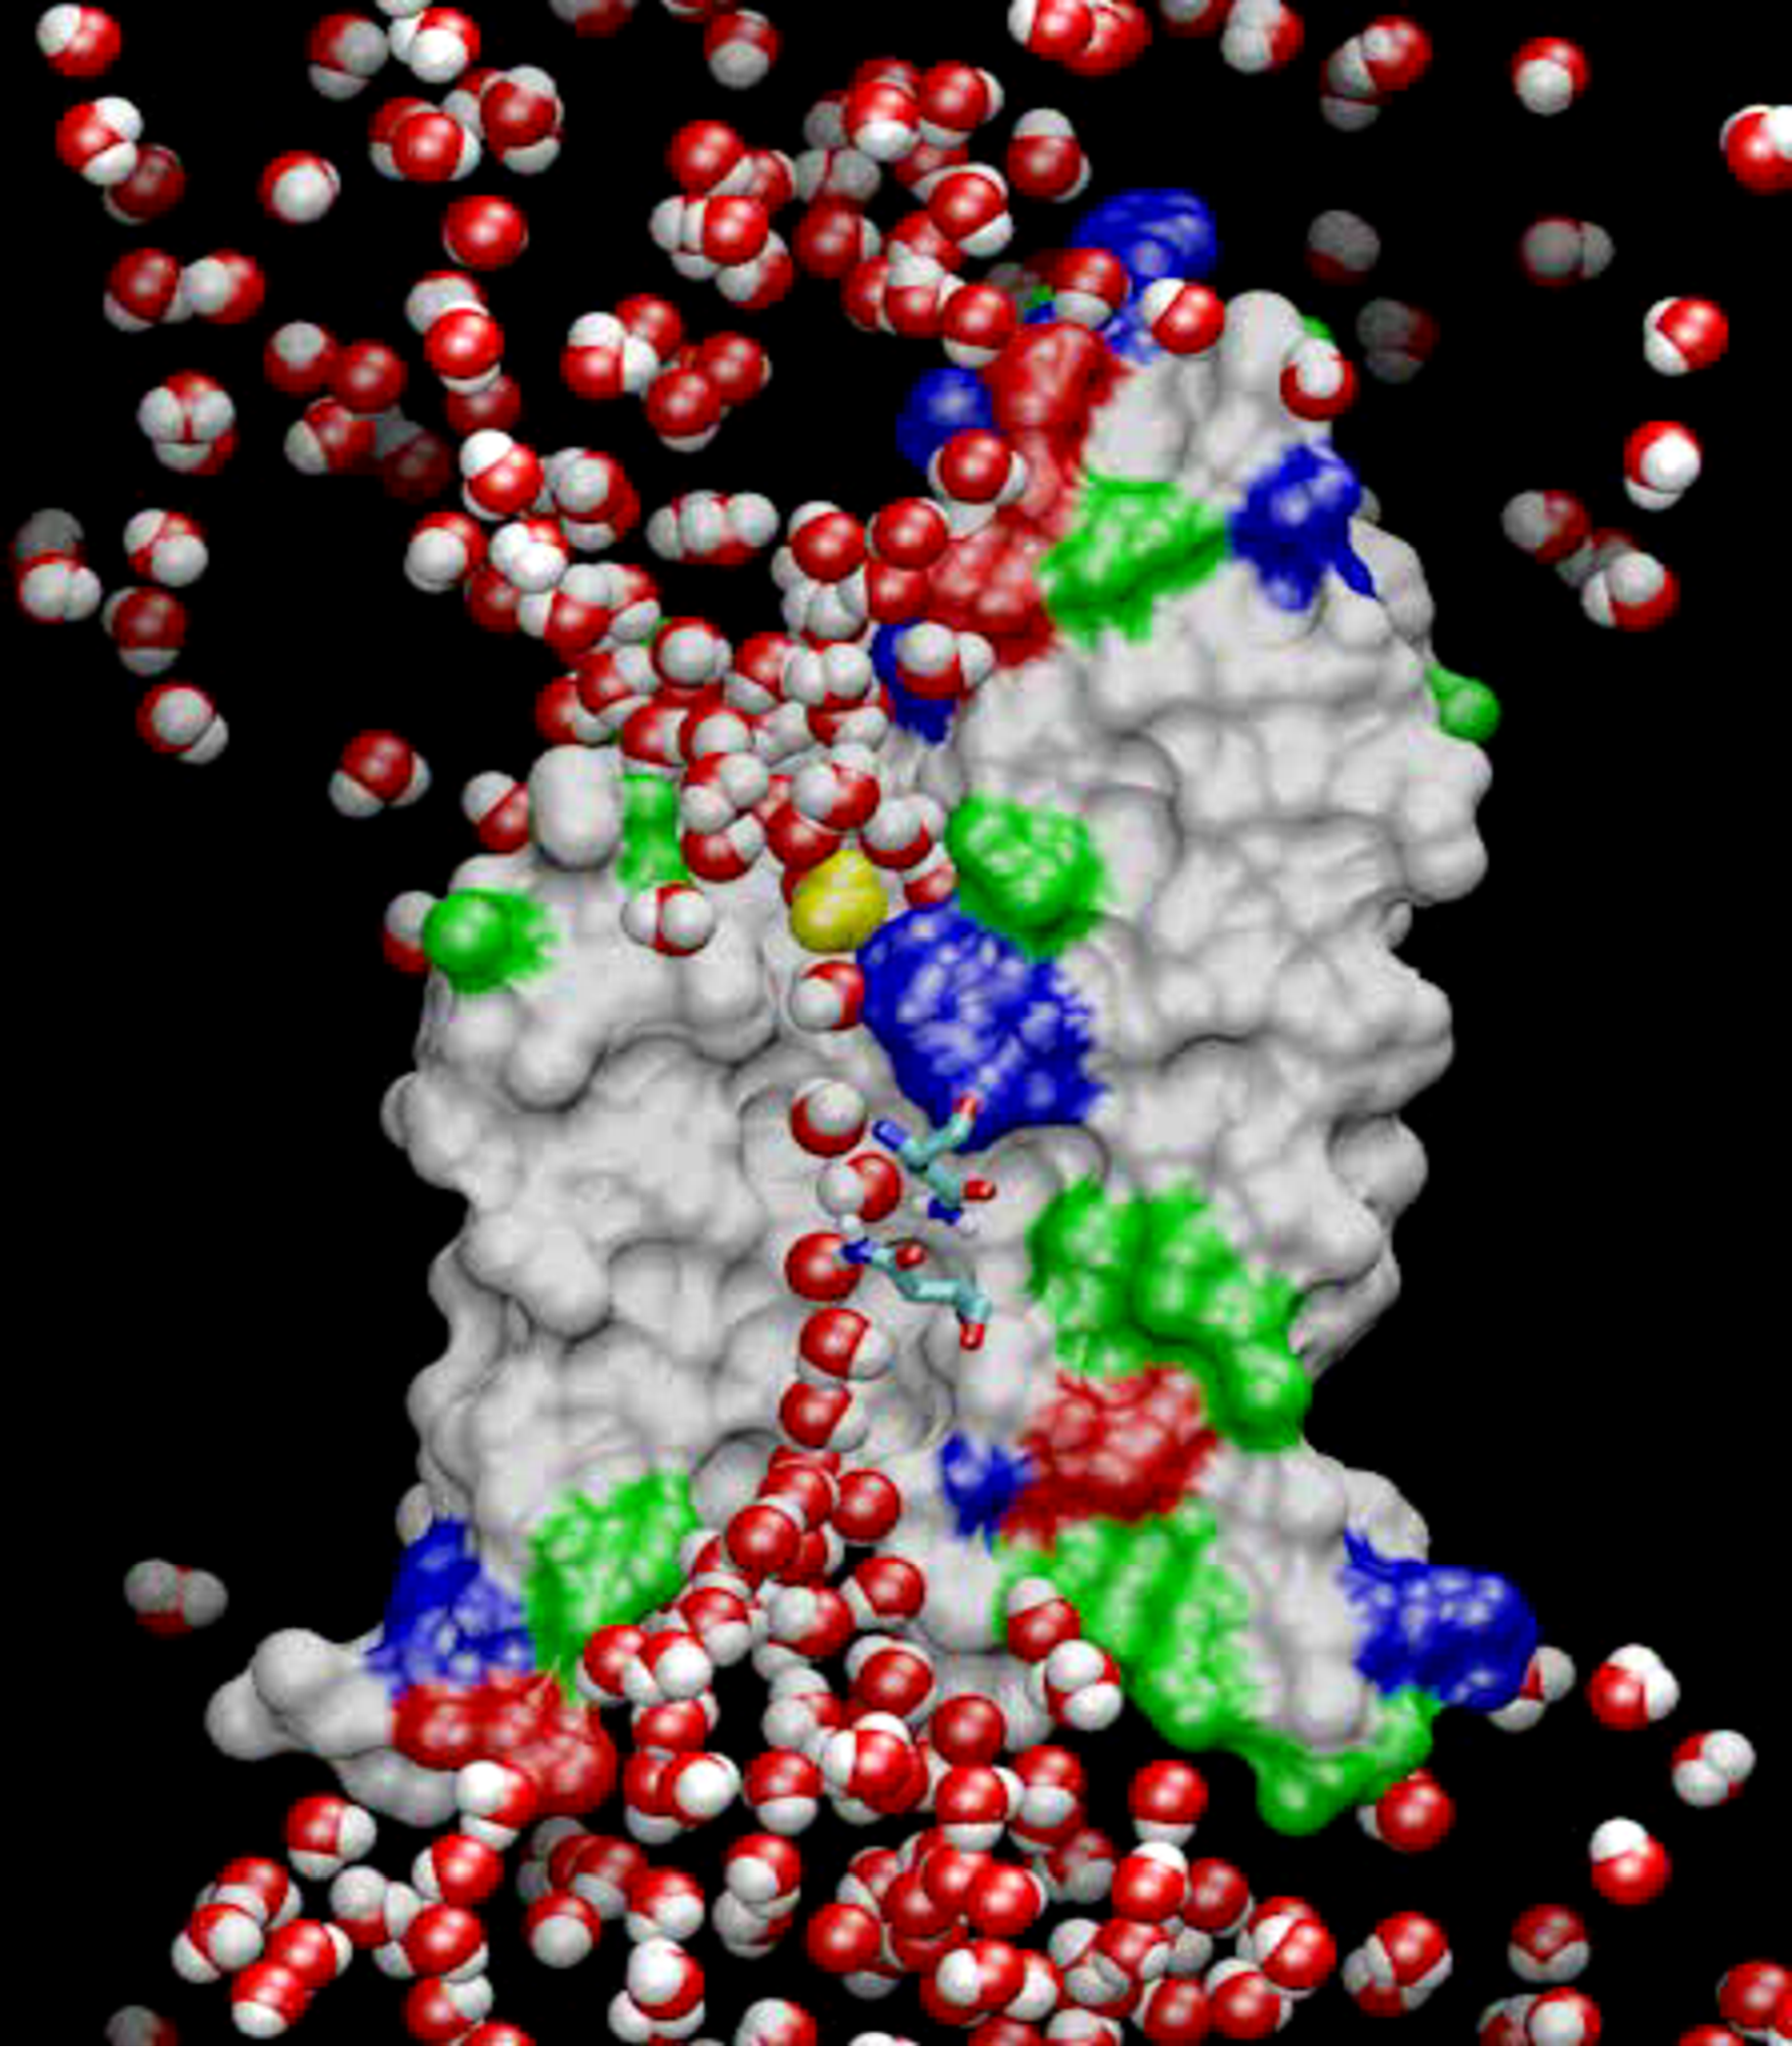
\includegraphics[width=\textwidth]{figures/namd.pdf} \end{center}
  \vfill
  \end{columns}
\end{frame}

\begin{frame}[t]
\frametitle{Spatial Decomposition Via Charm}
  \begin{columns}
  \column{.4\textwidth}
  \begin{center} 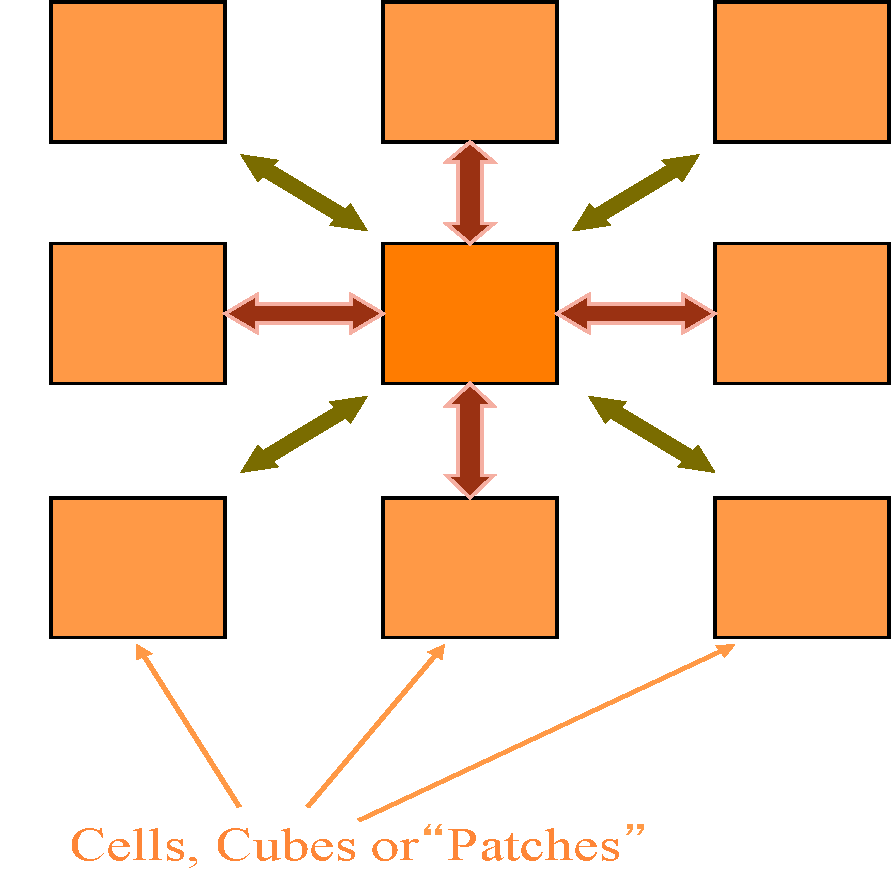
\includegraphics[width=0.8\textwidth]{figures/namd_decomp.pdf} \end{center}
  \column{.6\textwidth}
  \begin{itemize}
    \item Atoms distributed to cubes based on their location
    \pause
    \item Size of each cube :
    \begin{itemize}
      \item Just a bit larger than cut-off radius
      \item Communicate only with neighbors
      \item Work: for each pair of nbr objects
    \end{itemize}
    \item C/C ratio: O(1)
    \pause
    \item However: 
    \begin{itemize}
      \item Load imbalance
      \item Limited parallelism
    \end{itemize}
  \end{itemize}
  \pause
  \textcolor{red}{Charm++ is useful to handle this case}
  \end{columns}
\end{frame}

\begin{frame}[t]
\frametitle{Object Based Parallelization for MD}
\framesubtitle{Force Decomposition + Spatial Decomposition}
  \begin{columns}
  \column{.4\textwidth}
  \begin{center} 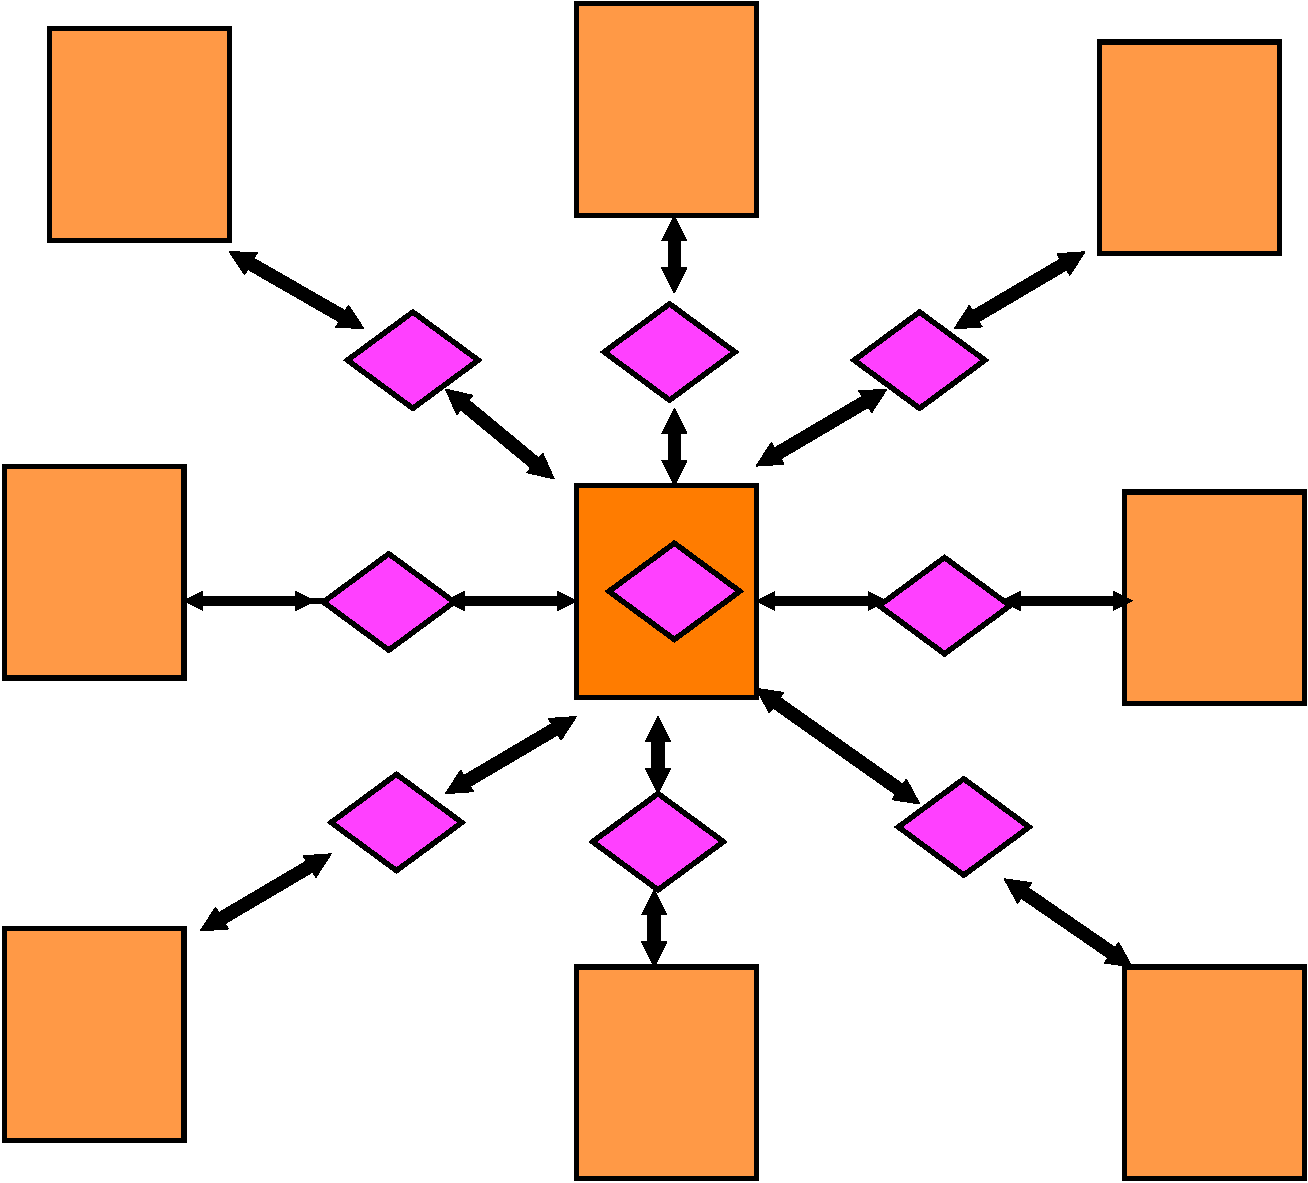
\includegraphics[width=0.8\textwidth]{figures/namd_decomp2.pdf} \end{center}
  \column{.6\textwidth}
  \begin{itemize}
    \item Now, we have many objects to load balance:
    \begin{itemize}
      \item Each diamond can be  assigned to any proc.
      \item Number of diamonds (3D): 14*Number of Patches
    \end{itemize}
    \pause
    \item 2-away variation:
    \begin{itemize}
      \item Half-size cubes
      \item Communicate only with neighbors
      \item 5 x 5 x 5 interactions
    \end{itemize}
    \pause
    \item 3-away interactions: 7 x 7 x 7
  \end{itemize}
  \end{columns}
\end{frame}

\begin{frame}[t]
\frametitle{NAMD Parallelization Using Charm++}
The computation is decomposed into ``natural'' objects of the application, which
are assigned to processors by Charm++ RTS
  \begin{center} 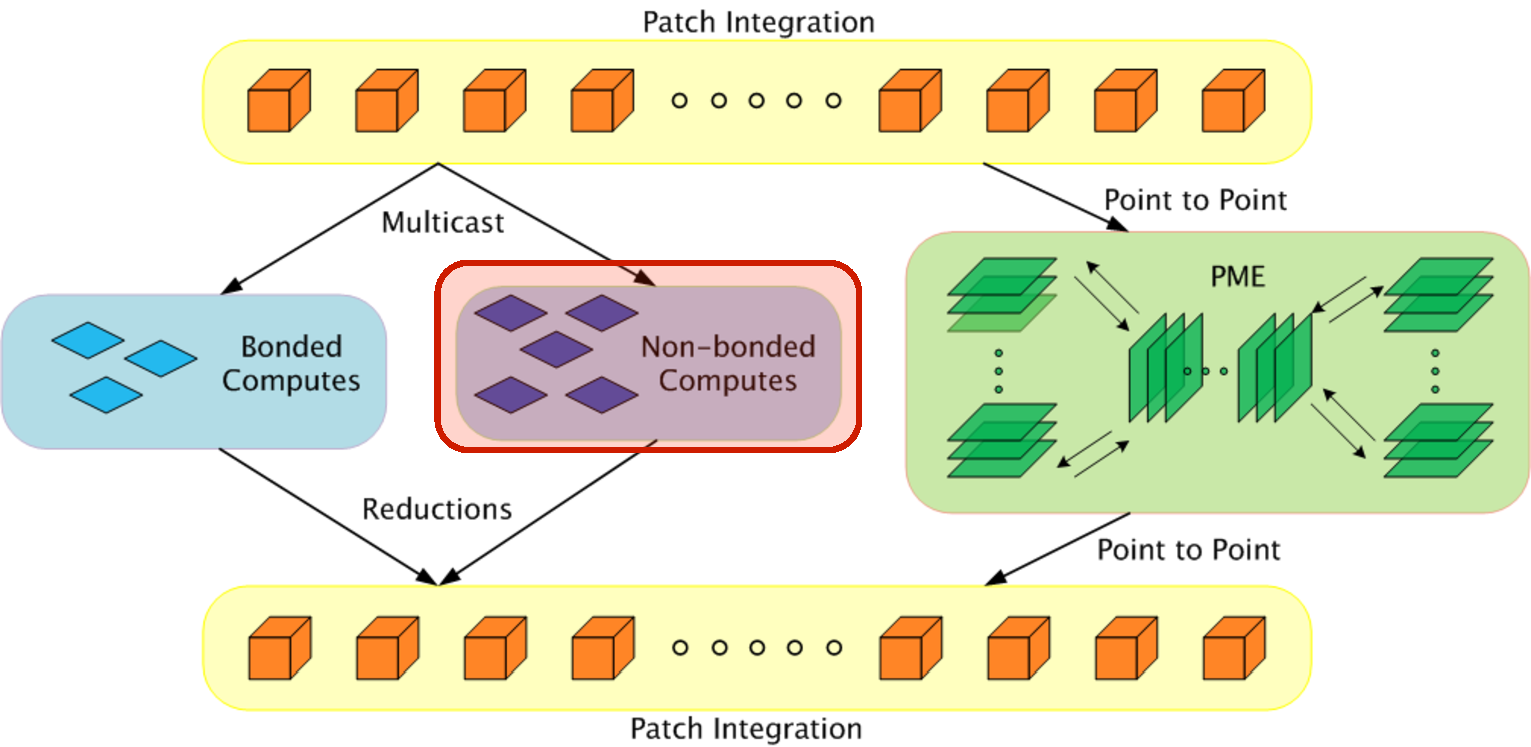
\includegraphics[width=\textwidth]{figures/md_parallelize.pdf} \end{center}
\end{frame}

\begin{frame}[t]
\frametitle{NAMD Projections}
  \begin{center} 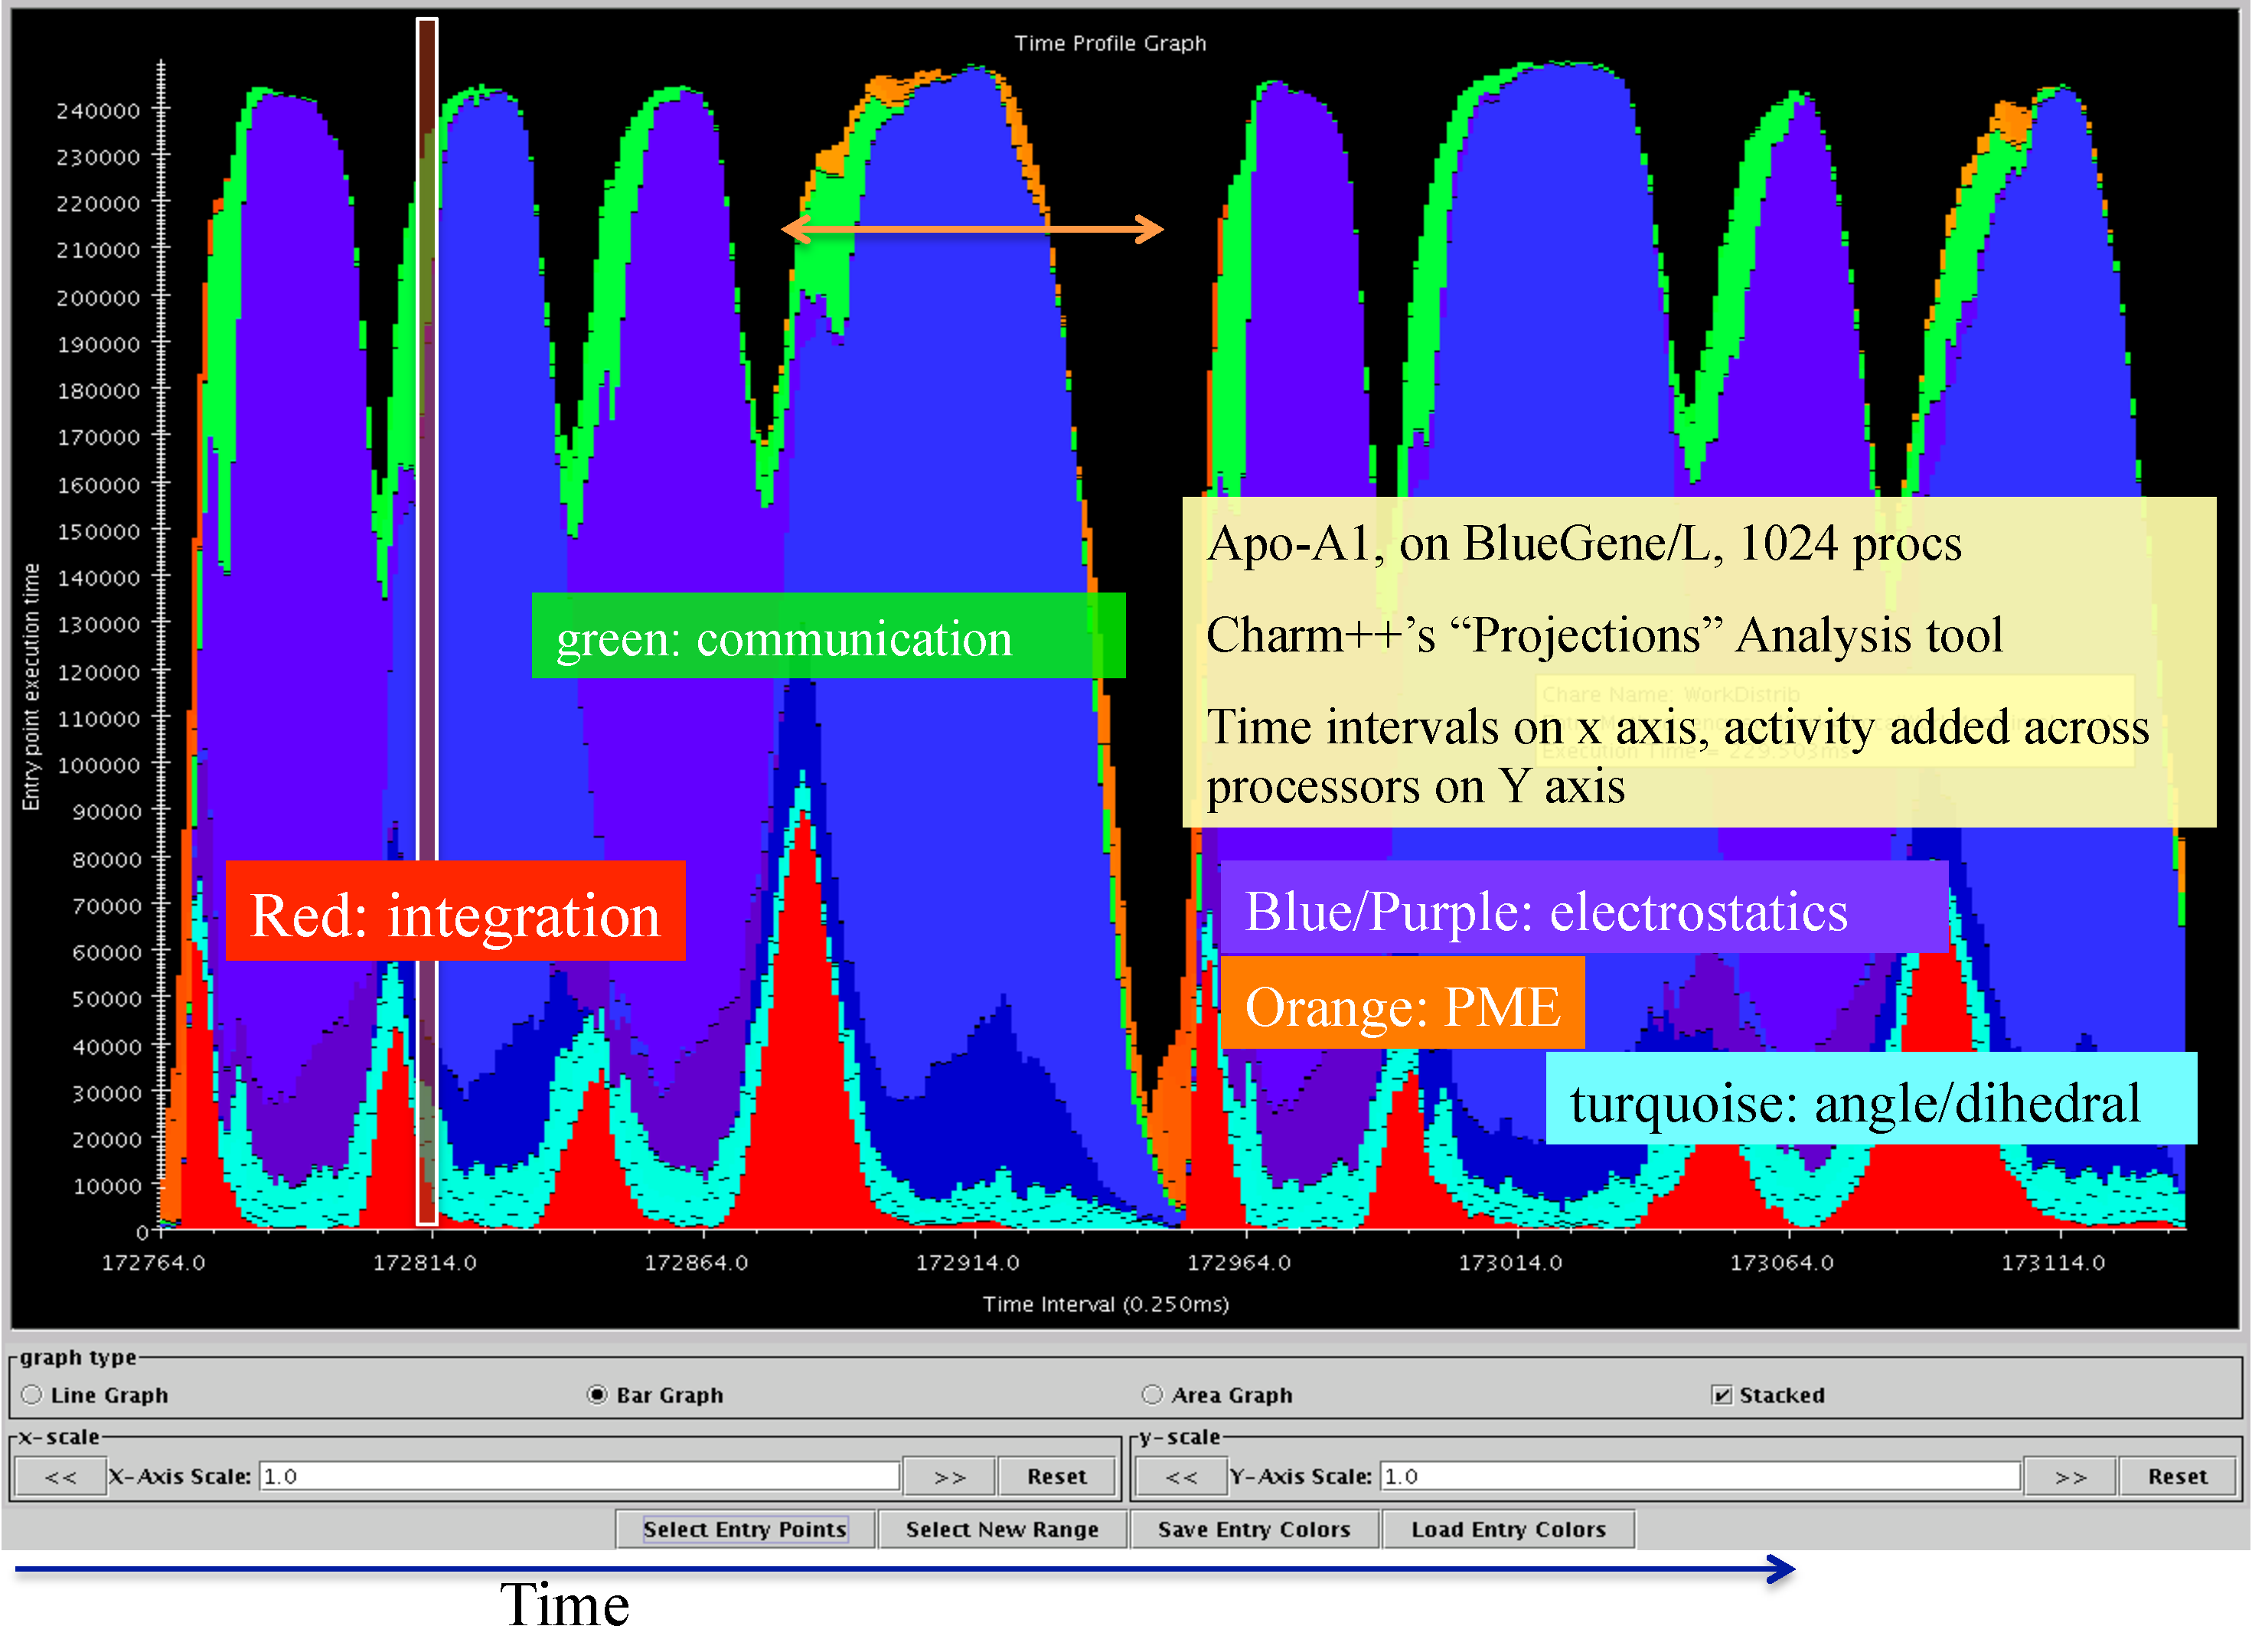
\includegraphics[width=.9\textwidth]{figures/namd_projection.pdf} \end{center}
\end{frame}

\begin{frame}[t]
\frametitle{NAMD Performance on IBM Blue Gene/P}
  \begin{center} 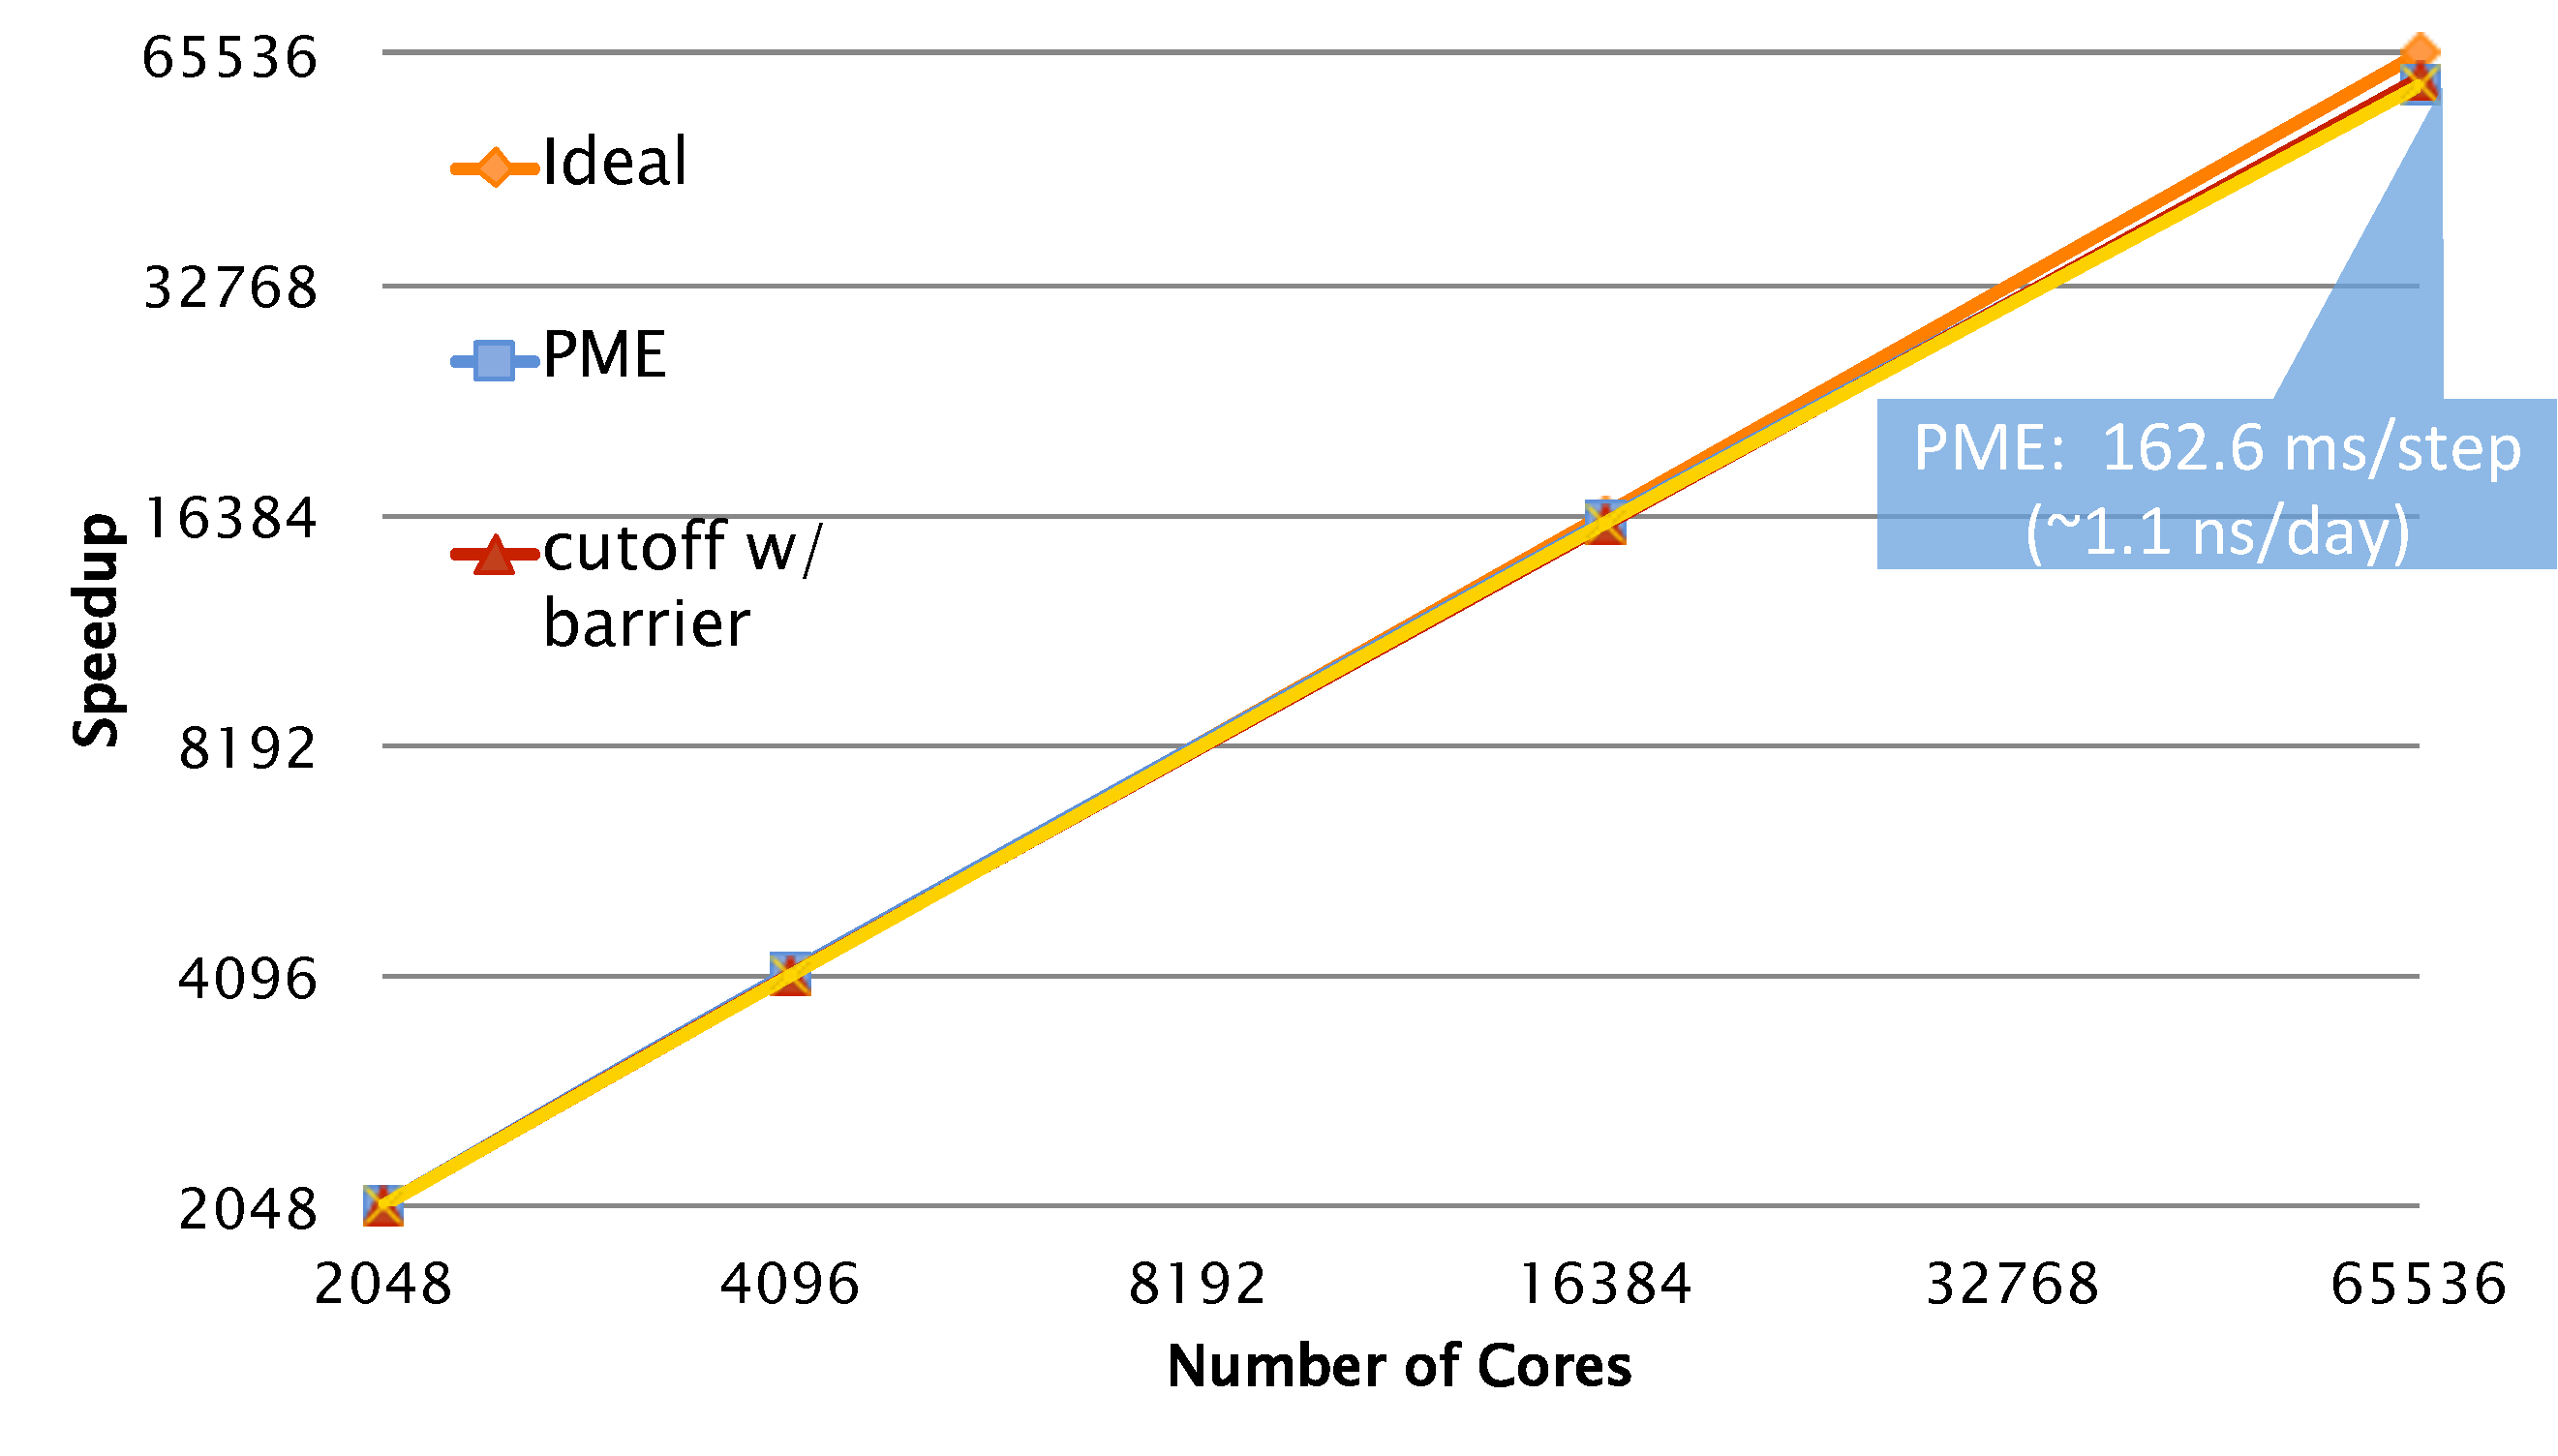
\includegraphics[width=\textwidth]{figures/namd_bgp.pdf} \end{center}
\end{frame}

\begin{frame}[t]
\frametitle{NAMD Performance on Titan}
  \begin{center} 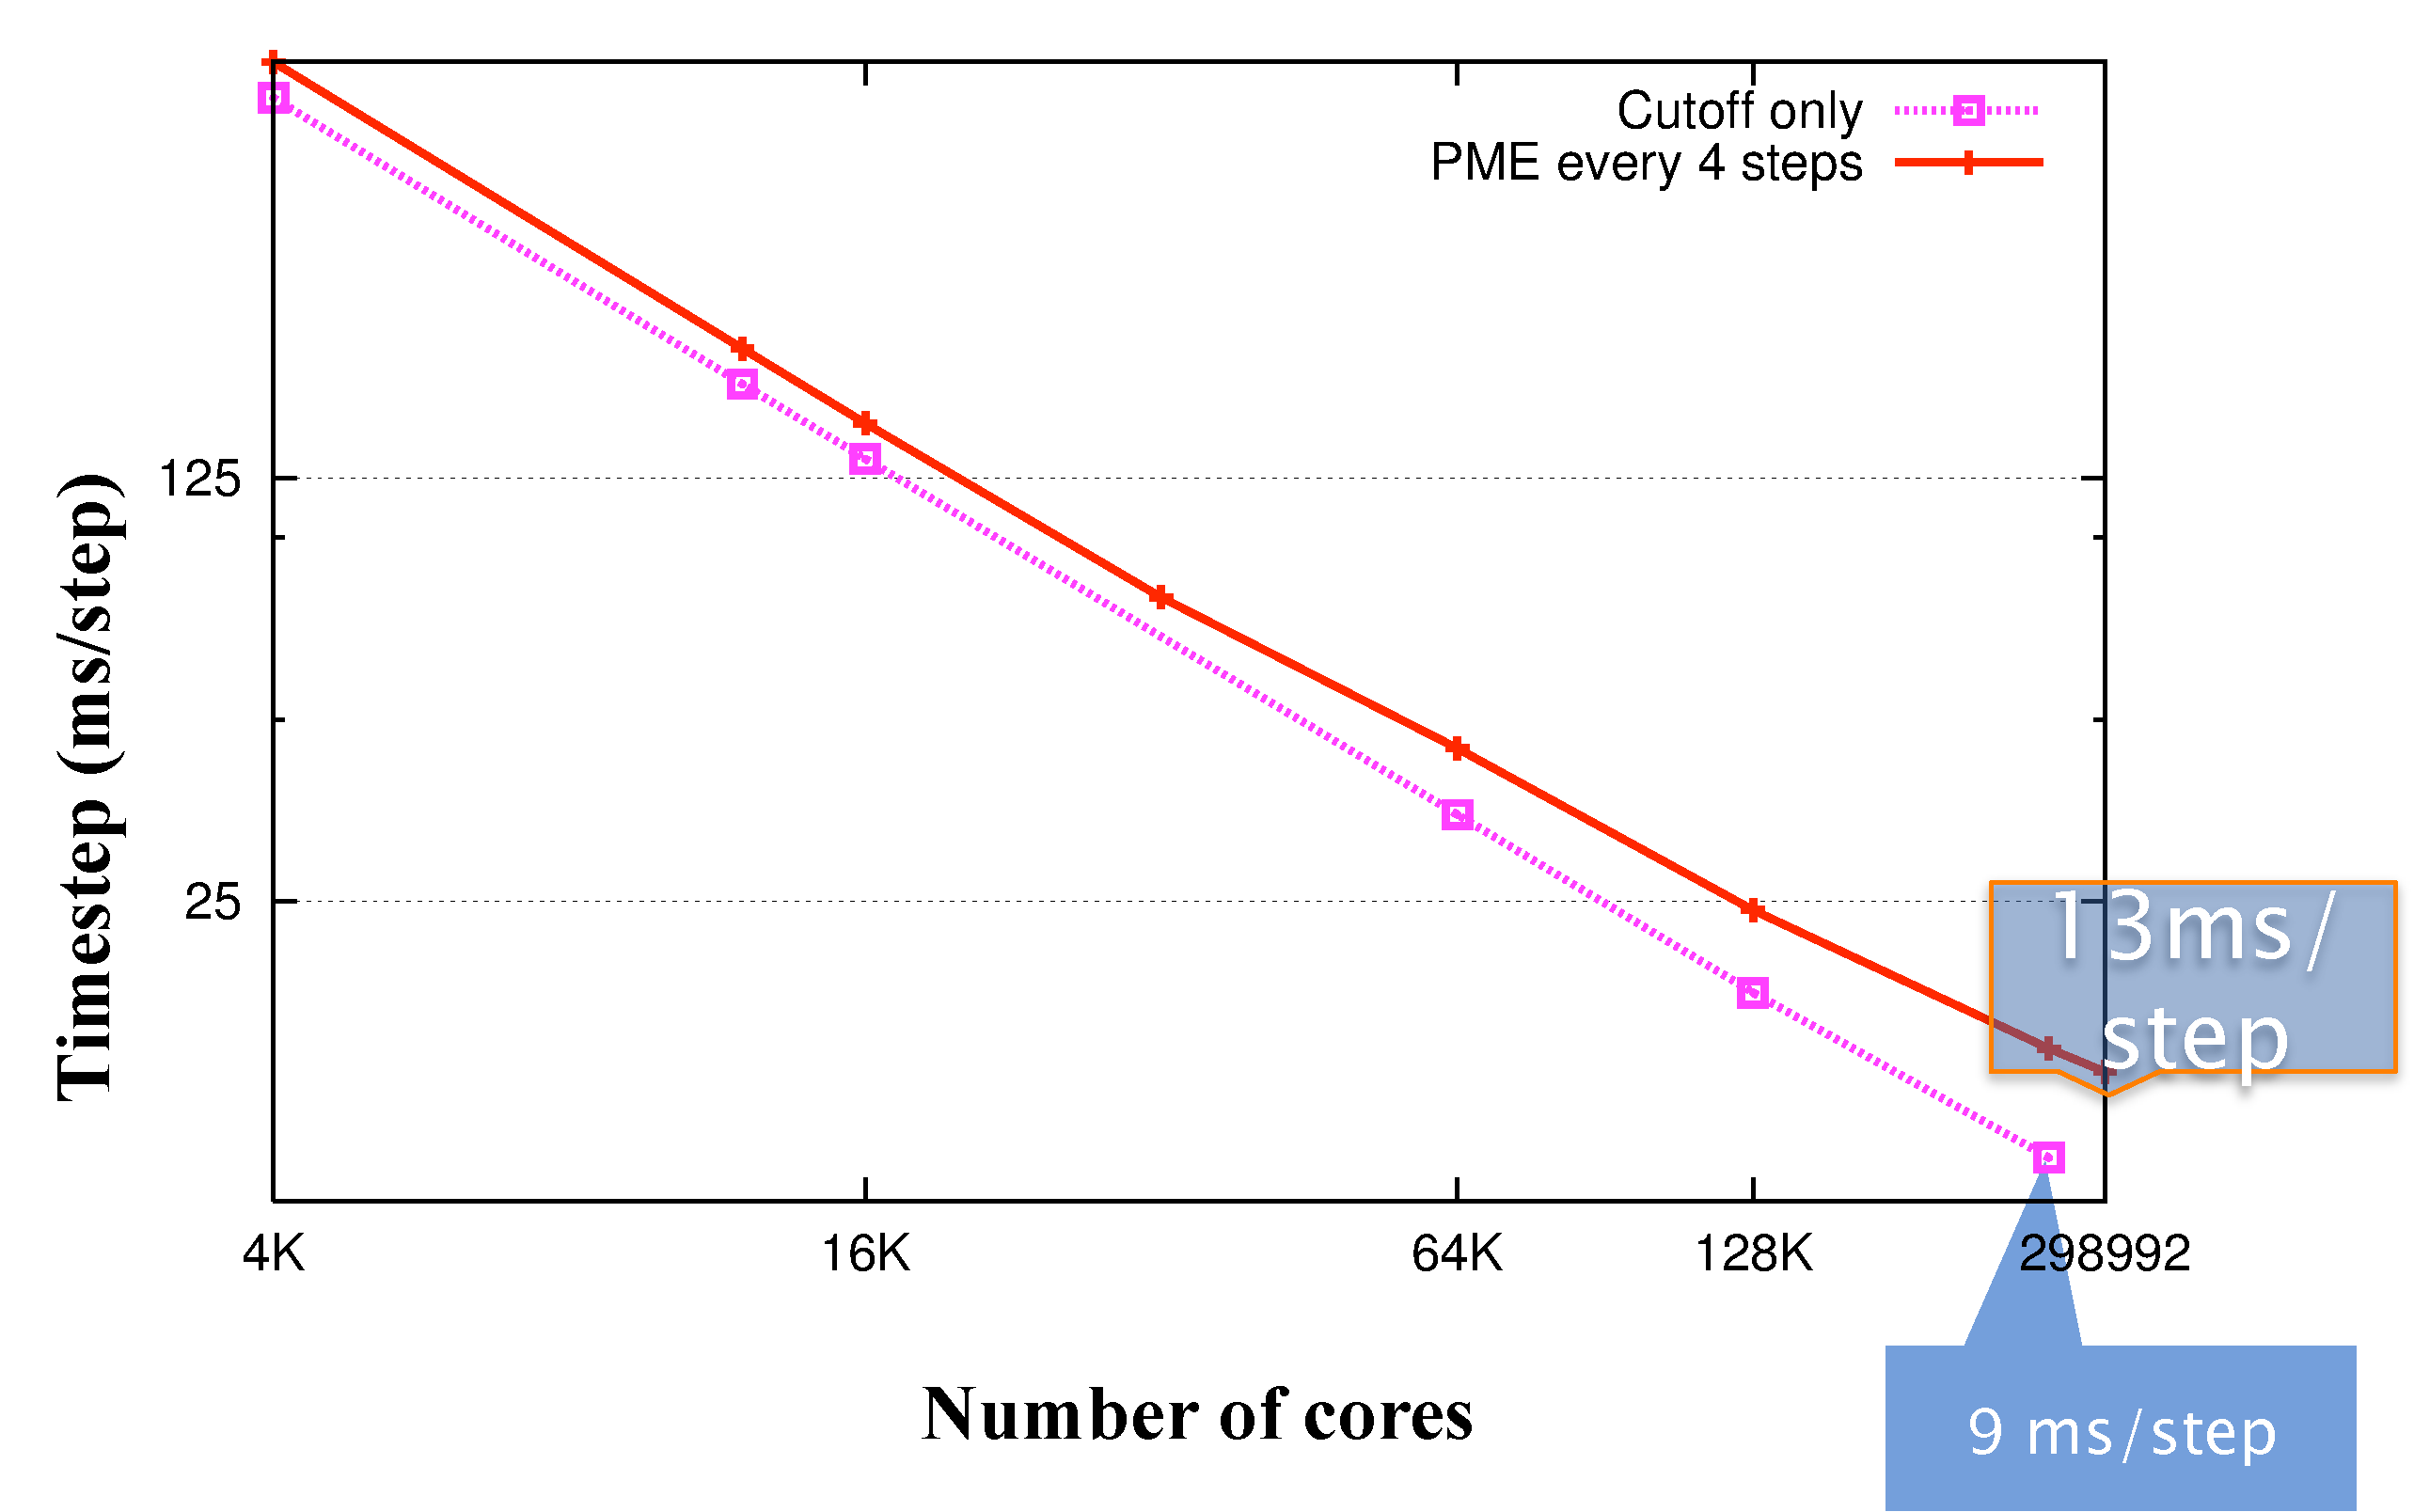
\includegraphics[width=.9\textwidth]{figures/namd_titan.pdf} \end{center}
\end{frame}

\begin{frame}[t]
\frametitle{ChaNGa: Parallel Gravity}
  \begin{itemize}
    \item Collaborative project (NSF)
    \begin{itemize} 
        \item with Tom Quinn, Univ. of Washington
    \end{itemize}
    \pause
    \item Evolution of Universe and Galaxy Formation
    \item Gravity, gas dynamics
    \pause
    \item Barnes-Hut tree codes
    \begin{itemize} 
      \item Oct tree is natural decomposition
      \item Geometry has better aspect ratios, so you ``open” up fewer nodes
      \item But is not used because it leads to bad load balance
      \item Assumption: one-to-one map between sub-trees and PEs
      \item Binary trees are considered better load balanced
    \end{itemize}
    \pause
    \item With Charm++: Use Oct-Tree, and let Charm++ map subtrees to processors
  \end{itemize}
\end{frame}

\begin{frame}[t]
\frametitle{ChaNGa: Control Flow}
  \begin{center} 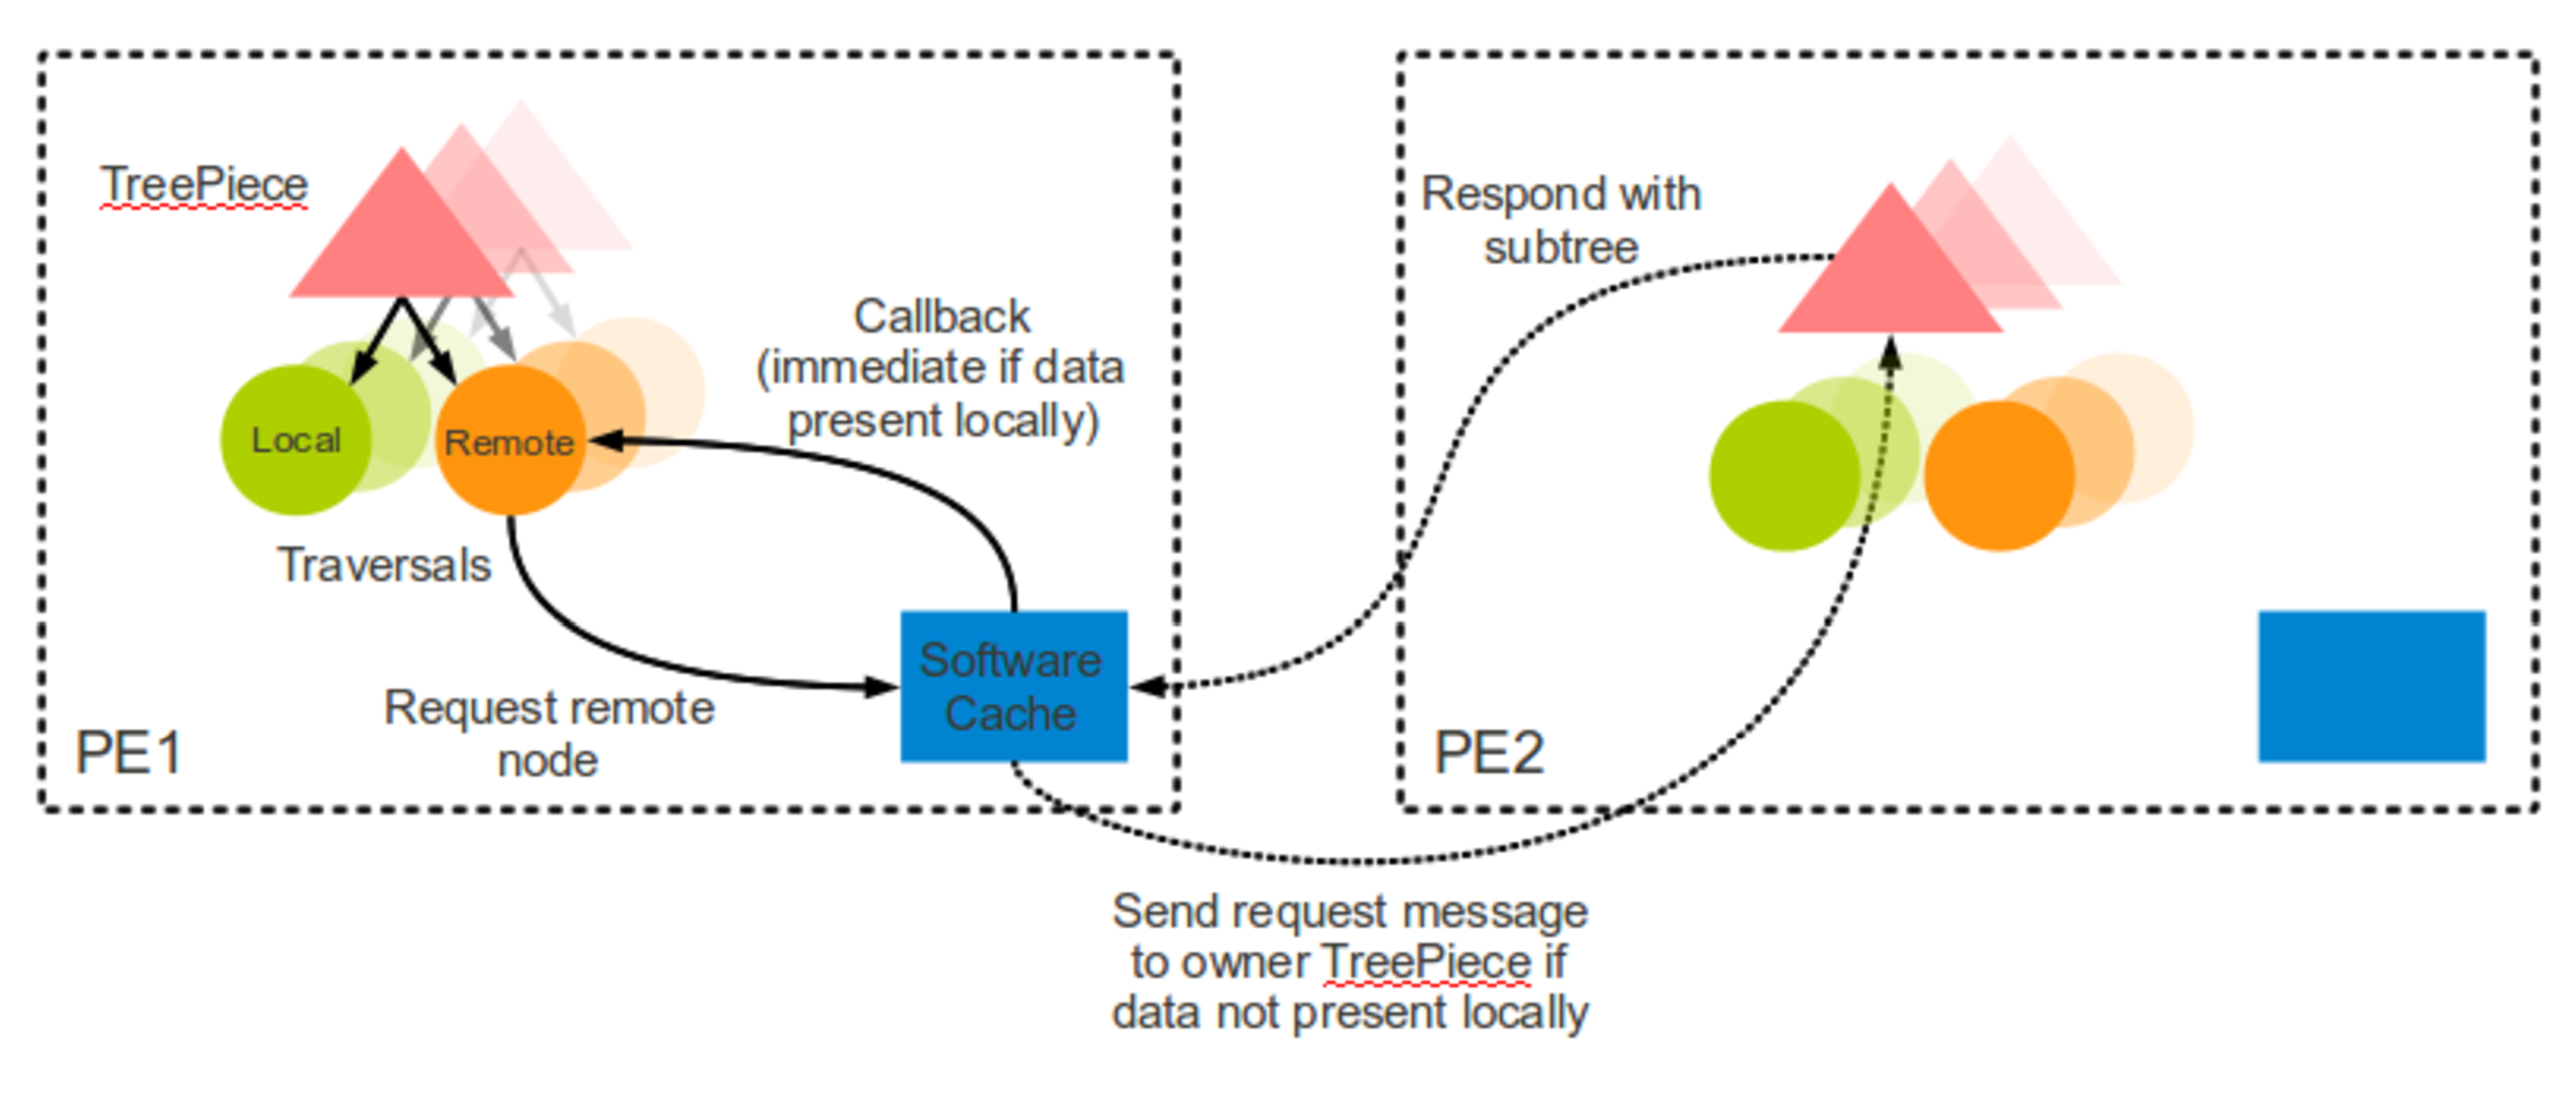
\includegraphics[width=\textwidth]{figures/changa.pdf} \end{center}
\end{frame}

\begin{frame}[t]
\frametitle{OpenAtom: MD with quantum effects}
  \begin{columns}
  \column{.5\textwidth}
    \begin{itemize}
      \item Much more fine-grained:
      \begin{itemize}
        \item Each electronic state is modeled with a large array
      \end{itemize}
      \pause
      \item Collaboration with:
      \begin{itemize}
        \item G. Martyna (IBM) 
        \item M. Tuckerman (NYU)
      \end{itemize}
      \pause
    \item Using Charm++ virtualization, we can efficiently scale small (32 molecule) systems to thousands of processors
  \end{itemize}
  \column{.5\textwidth}
  \begin{center} 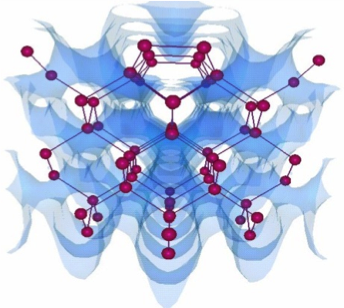
\includegraphics[width=.5\textwidth]{figures/openatom1.png}\\
  \textcolor{red}{Semiconductor Surfaces}\end{center}
  \begin{center} 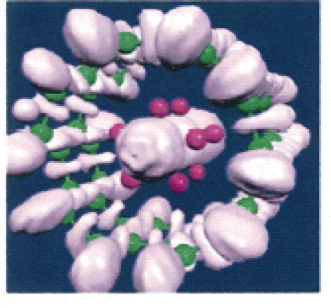
\includegraphics[width=.5\textwidth]{figures/openatom2.png}\\
  \textcolor{red}{Nanowires}\end{center}
  \end{columns}
\end{frame}


\begin{frame}[t]
\frametitle{OpenAtom: Decomposition and Computation Flow}
  \begin{center} 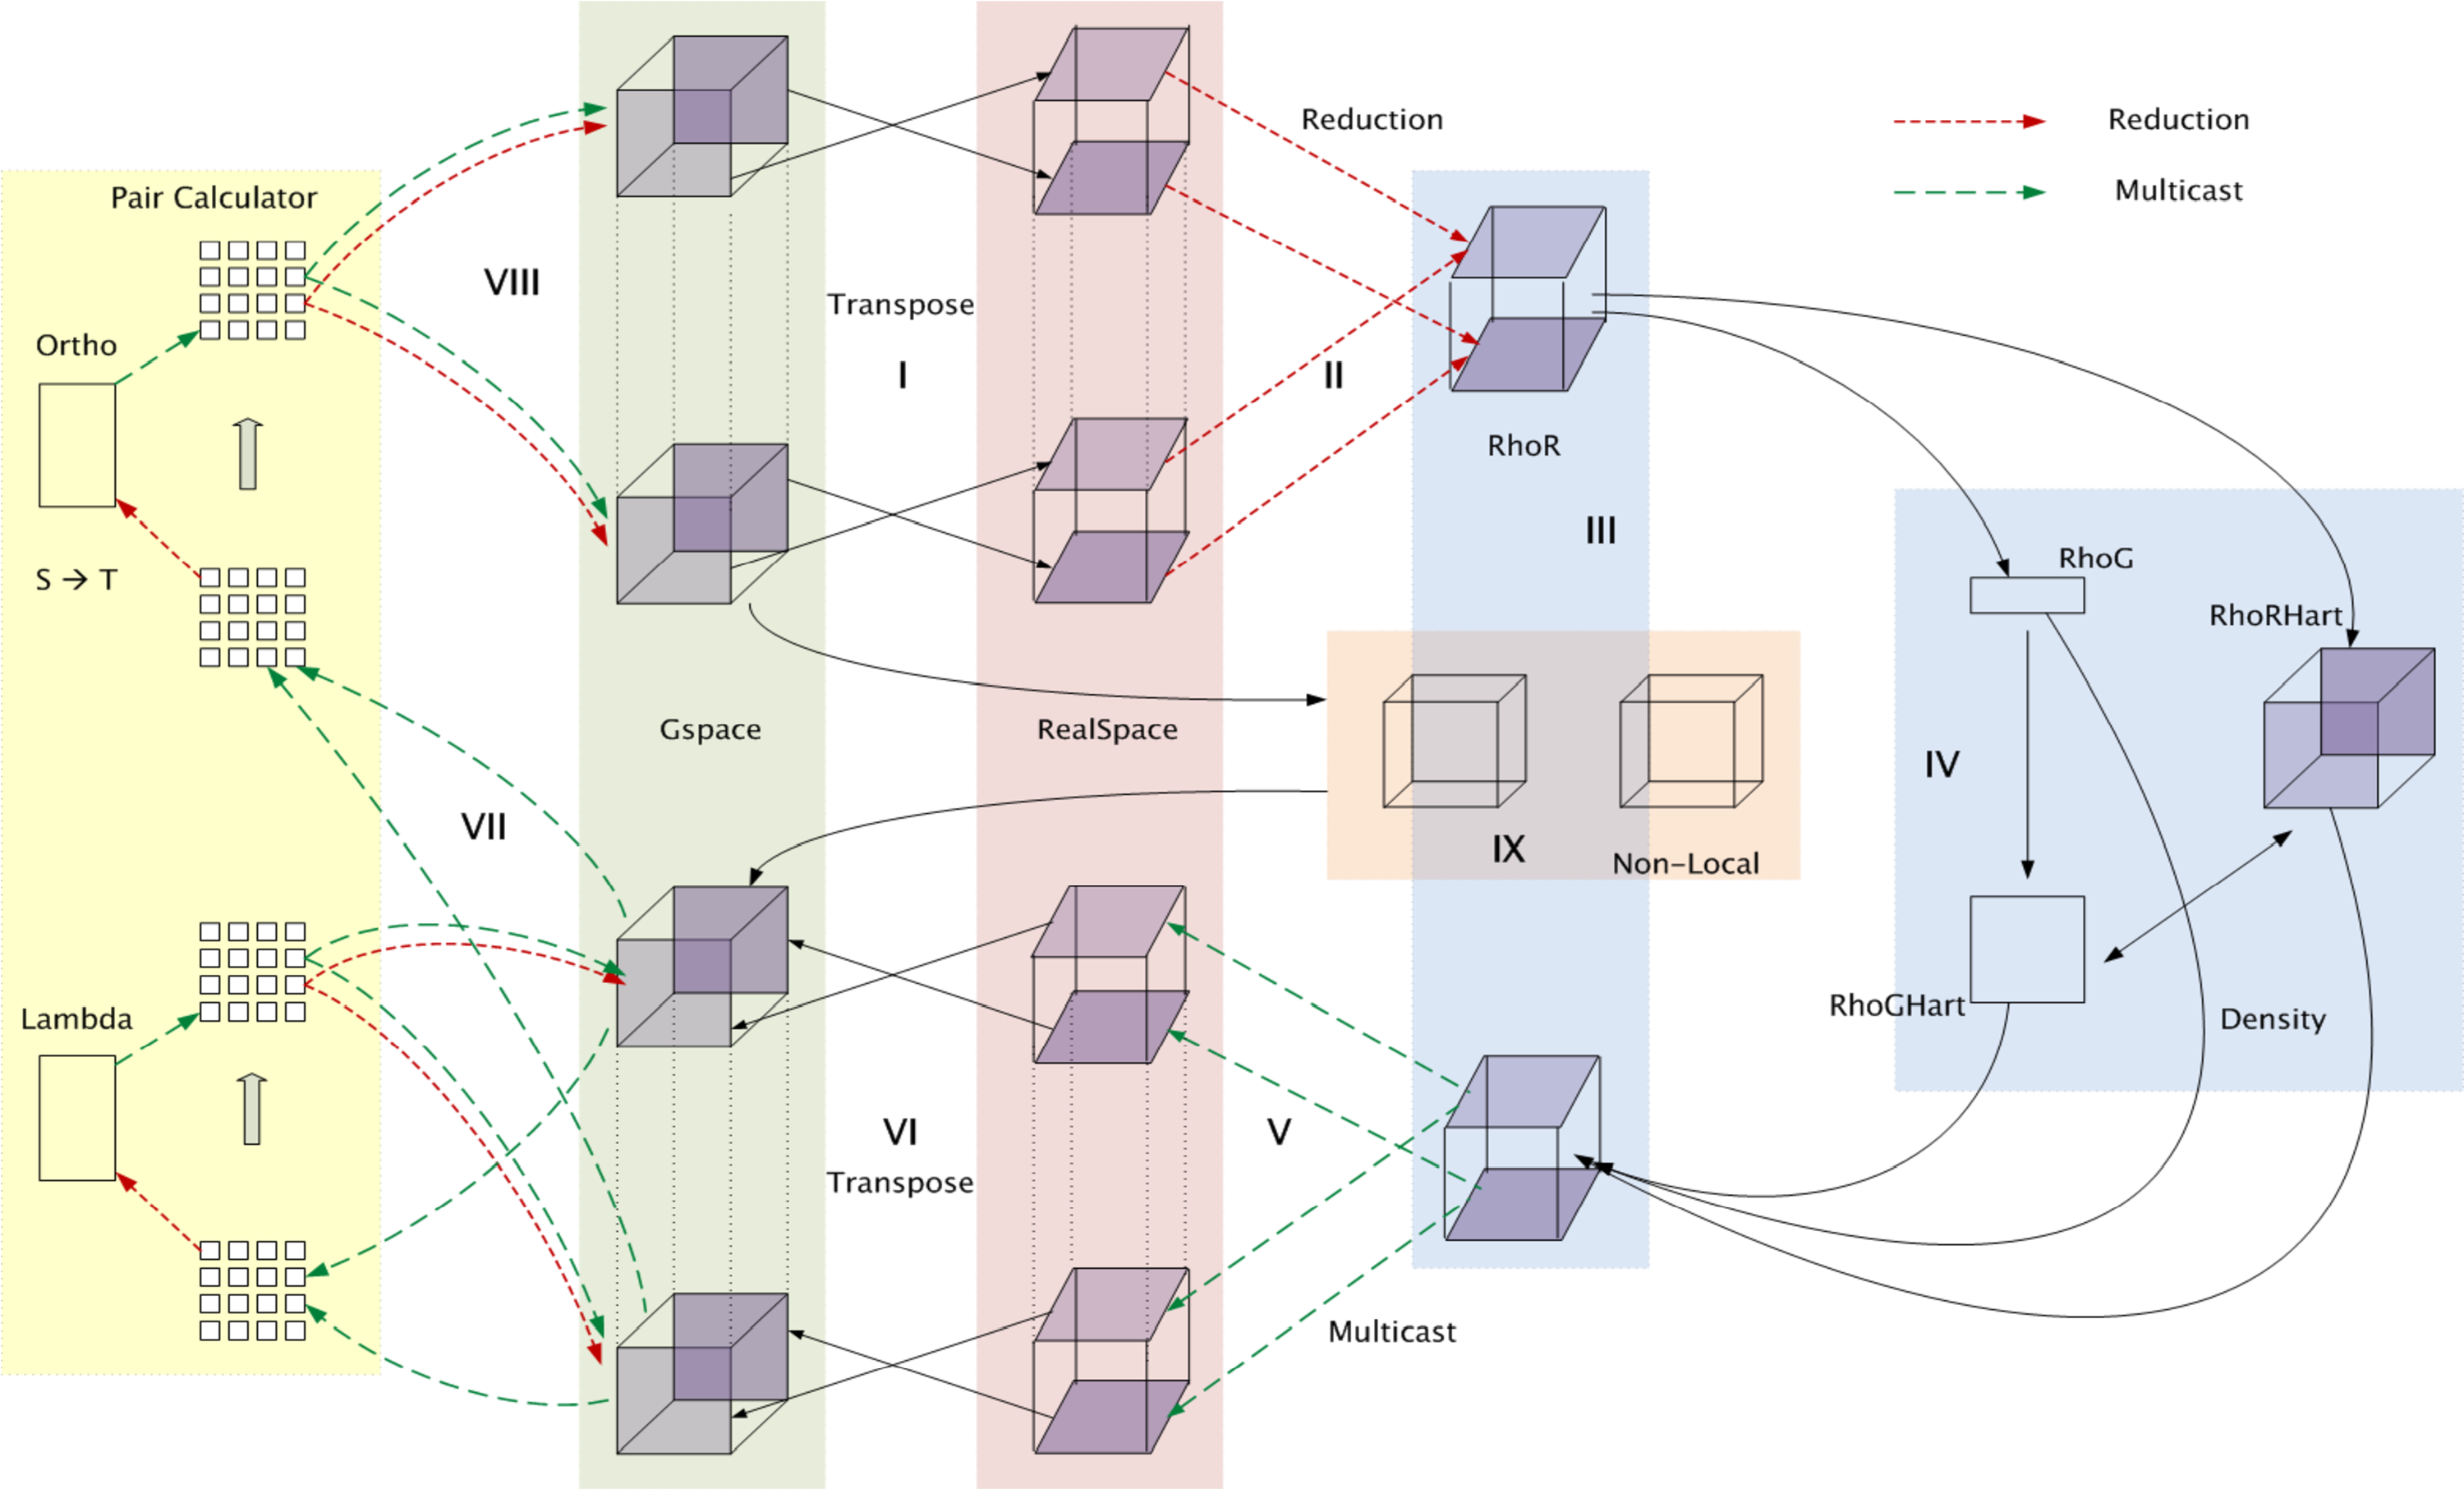
\includegraphics[width=\textwidth]{figures/openatom_array.pdf} \end{center}
\end{frame}

\begin{frame}[t]
\frametitle{OpenAtom: Topology Aware Mapping of Objects}
  \begin{center} 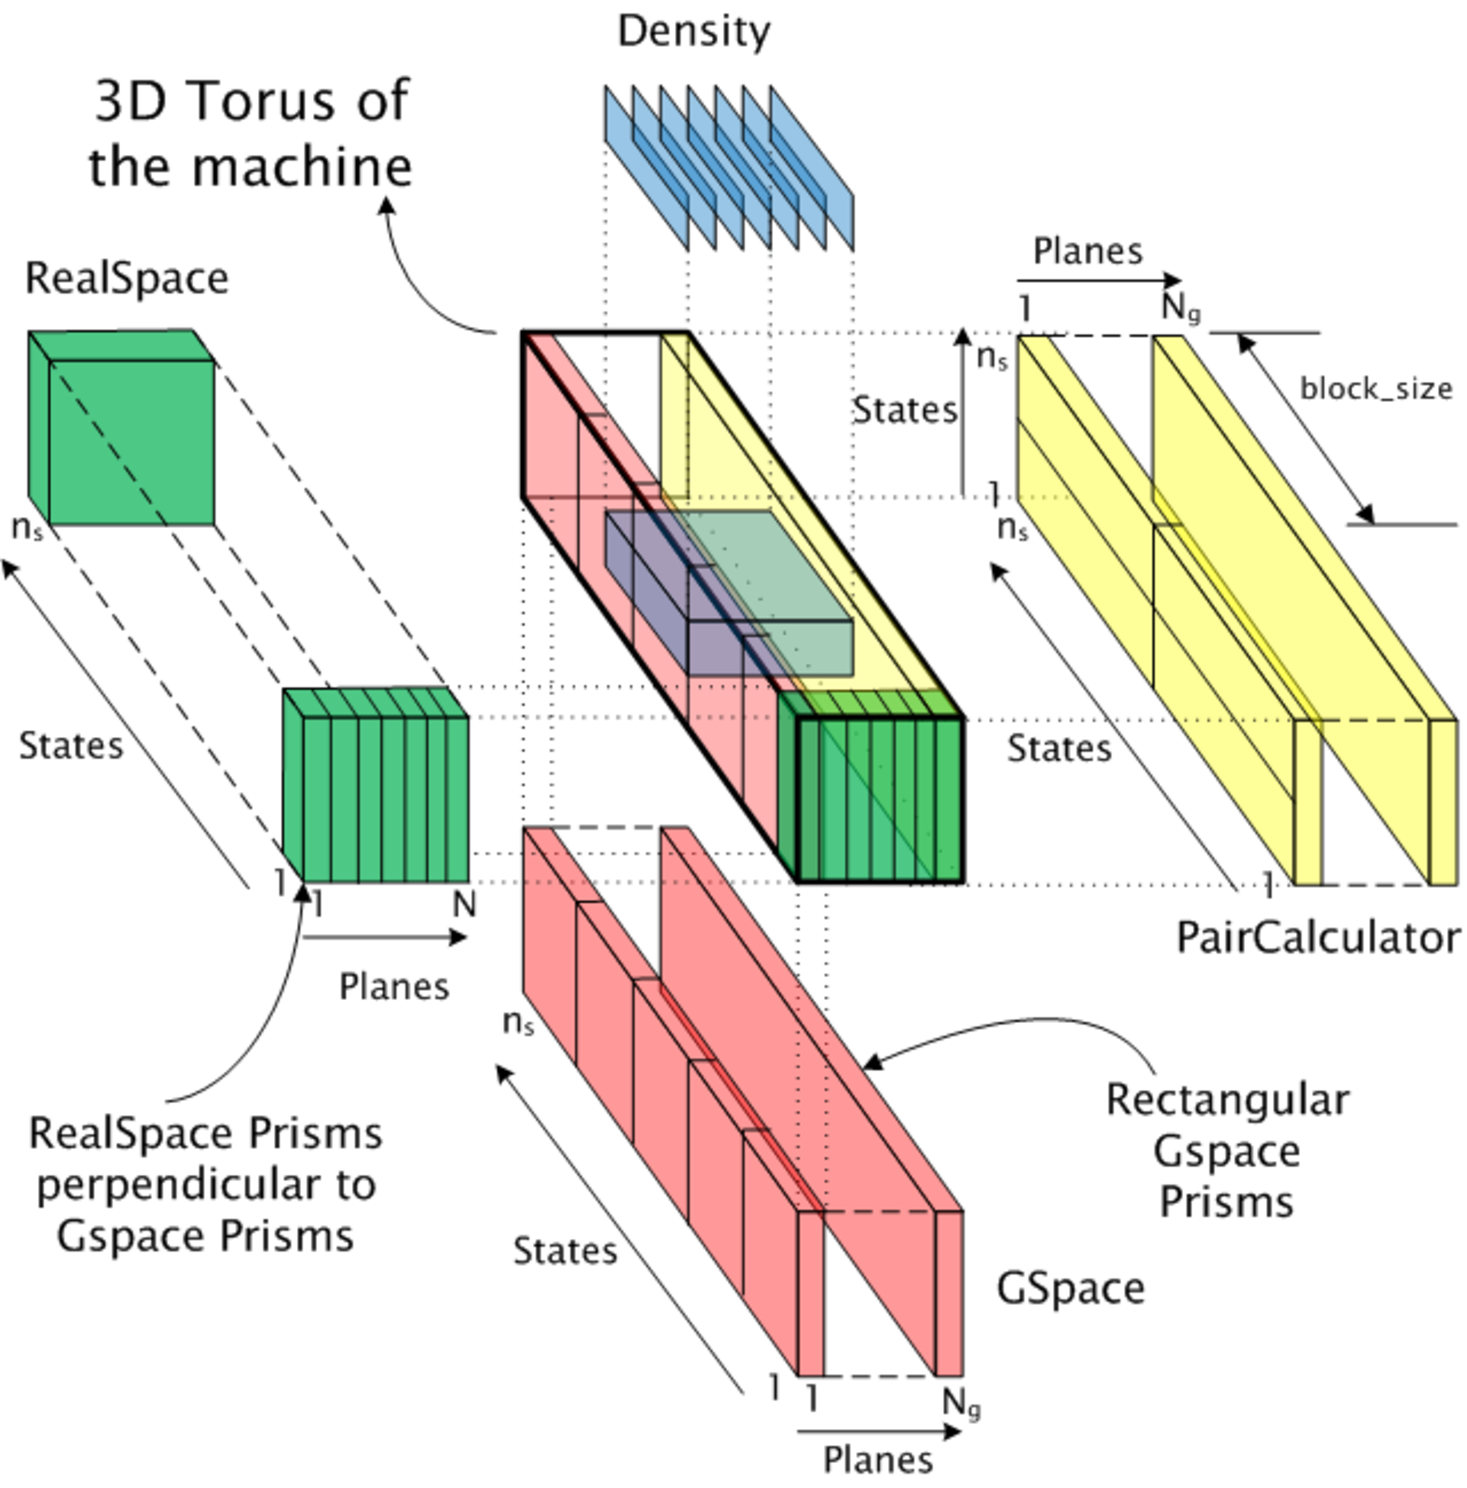
\includegraphics[width=.45\textwidth]{figures/openatom_topo.pdf} \end{center}
  Object based decomposition provides new degrees of freeedom to easily try
  different mappings of objects to processors, to help minimize contention

\end{frame}

\section[Charm++]{Charm++ Syntax}
\transition{Charm++}\begin{frame}
  \frametitle{Charm++ File structure}
  \begin{itemize}
    \item C++ objects (including Charm++ objects)
      \begin{itemize}
      \item Defined in regular \texttt{.h} and \texttt{.cpp} files
      \end{itemize}
    \item Chare objects, entry methods (asynchronous methods)
      \begin{itemize}
      \item Defined in \texttt{.ci} file
      \item Implemented in the \texttt{.cpp} file
      \end{itemize}
  \end{itemize}
  \begin{center}
    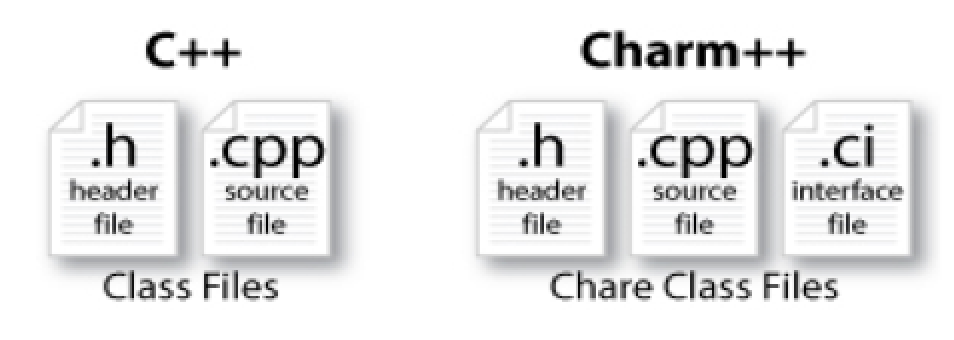
\includegraphics[width=0.6\textwidth]{figures/charmFiles.png}
  \end{center}
\end{frame}

\begin{frame}[fragile]
  \frametitle{Charm Interface: Modules}
  \begin{itemize}
    \item Charm++ programs are organized as a collection of modules
    \item Each module has one or more chares
    \item The module that contains the \textit{mainchare}, is declared as the
      \texttt{mainmodule}
    \item Each module, when compiled, generates two files:
      \code{<modulename>.decl.h} and \code{<modulename>.def.h}
  \end{itemize}
  \begin{center}
  \begin{lstlisting}
    [main]module <modulename> {
      //... chare definitions ...
    };
  \end{lstlisting}
  \end{center}
\end{frame}

\begin{frame}[fragile]
  \frametitle{Charm Interface: Chares}
  \begin{itemize}
    \item Chares are parallel objects that are managed by the RTS
    \item Each chare has a set \textit{entry methods}, which are asynchronous
      methods that may be invoked remotely
    \item The following code, when compiled, generates a C++ class
      \code{CBase\_<charename>} that encapsulates the RTS object
    \item This generated class is extended and implemented in the \texttt{.cpp}
      file
  \end{itemize}
  \begin{lstlisting}
    [main]chare <charename> {
      //... entry method definitions ...
    };

    class <charename> : public CBase_<charename> {
      //... entry method implementations ...
    };
  \end{lstlisting}
\end{frame}

\begin{frame}[fragile]
  \frametitle{Charm Interface: Entry Methods}
  \begin{itemize}
  \item Entry methods are C++ methods that can be remotely and asynchronously
    invoked by another chare
  \end{itemize}
  \texttt{.ci} file:
  \begin{lstlisting}
    entry <charename>(); /* constructor entry method */
    entry void foo();
    entry void bar(int param);
  \end{lstlisting}
  \texttt{.cpp} file:
  \begin{lstlisting}
    <charename>::<charename>() { /*... constructor code ...*/ }

    <charename>::foo() { /*... code to execute ...*/ }

    <charename>::bar(int param) { /*... code to execute ...*/ }
  \end{lstlisting}
\end{frame}

\begin{frame}[fragile]
   \frametitle{Charm Interface: \texttt{mainchare}}
   \begin{itemize}
     \item Execution begins with the \texttt{mainchare}'s constructor
     \item The \texttt{mainchare}'s constructor takes a pointer to
       system-defined class \code{CkArgMsg}
     \item \code{CkArgMsg} contains \code{argv} and \code{argc}
     \item The \texttt{mainchare} will often construct other parallel objects
       and then wait for them to finish
   \end{itemize}
\end{frame}

\begin{frame}[fragile]
  \frametitle{Creating a Chare}
  \begin{itemize}
    \item A chare declared as \code{chare <charename> \{...\};} can be
      instantiated by the following call:
  \end{itemize}
\begin{lstlisting}
CProxy_<charename>::ckNew(... constructor arguments ...);
\end{lstlisting}
  \begin{itemize}
  \item To communicate with this class in the future, a \textit{proxy} to it
    must be retained
  \end{itemize}
\begin{lstlisting}
CProxy_<charename> proxy = 
  CProxy_<charename>::ckNew(... constructor arguments ...);
\end{lstlisting}
\end{frame}

\begin{frame}[fragile]
  \frametitle{Chare Proxies}
  \begin{itemize}
  \item A chare's own proxy can be obtained through a special variable
    \code{thisProxy}
  \item Chare proxies can also be passed so chares can learn about others
  \item In this snippet, \code{<charename>} learns about a chare instance
    \code{main}, and then invokes a method on it:
  \end{itemize}
\texttt{.ci} file
\begin{lstlisting}
entry void foobar2(CProxy_Main main);
\end{lstlisting}
\texttt{.cpp} file
\begin{lstlisting}
<charename>::foobar2(CProxy_Main main) {
  main.foo();
}
\end{lstlisting}
\end{frame}

\begin{frame}[fragile]
   \frametitle{Charm Termination}
   \begin{itemize}
   \item There is a special system call \code{CkExit()} that terminates the
     parallel execution on all processors (but it is called on one processor)
     and performs the requisite cleanup
   \item The traditional \code{exit()} is insufficient because it only
     terminates one process, not the entire parallel job (and will cause a
     hang)
   \item \code{CkExit()} should be called when you can safely terminate the
     application (you may want to synchronize before calling this)
   \end{itemize}
\end{frame}

\begin{frame}
   \frametitle{Compiling a Charm++ Program}
   \begin{center}
     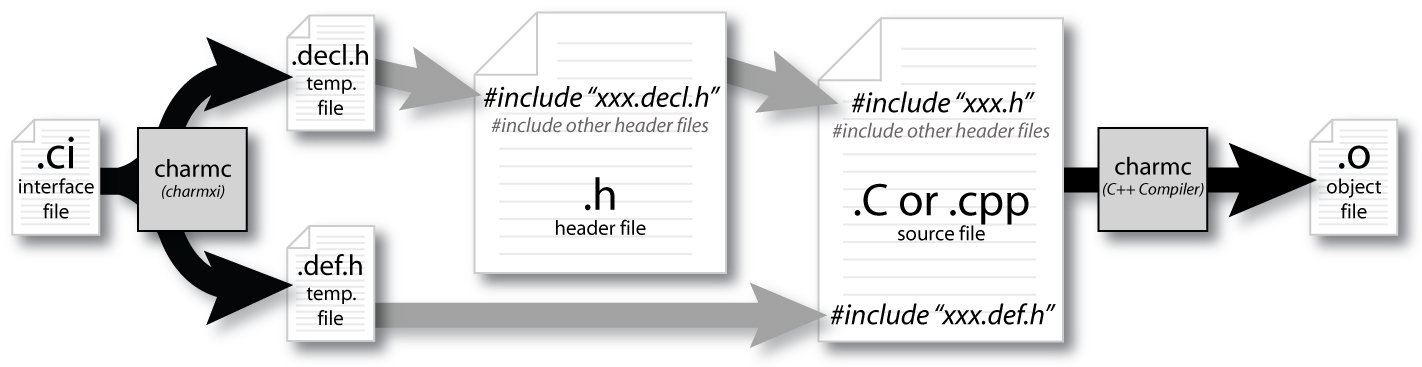
\includegraphics[width=0.9\textwidth]{figures/charmCompile.jpg}
   \end{center}
\end{frame}

\begin{frame}
  \frametitle{Building Charm++}
  \begin{itemize}
  \item git clone -b charm-6.5 git://charm.cs.uiuc.edu/charm.git
  \item ./build $<$TARGET$>$ $<$ARCH$>$ $<$OPTS$>$
  \item TARGET = Charm++, AMPI, bgampi, LIBS etc.
  \item ARCH = net-linux-x86\_64, pamilrts-bluegeneq etc.
  \item OPTS = --with-production, --enable-tracing, xlc, smp, -j8 etc.
  \end{itemize}
\end{frame}

\begin{frame}
  \frametitle{Hello World Example}
  \begin{itemize}
    \item Compiling
      \begin{itemize}
      \item \texttt{charmc hello.ci}
      \item \texttt{charmc -c hello.cpp}
      \item \texttt{charmc -o hello hello.o}
      \end{itemize}
    \item Running
      \begin{itemize}
      \item \texttt{./charmrun +p7 ./hello}
      \item The \texttt{+p7} tells the system to use seven cores
      \end{itemize}
    \end{itemize}
\end{frame}


\begin{frame}[fragile]
  \frametitle{Chare Creation Example: \texttt{.ci} file}
  \lstinputlisting{code/chareCreate.ci}
\end{frame}

\begin{frame}[fragile]
  \frametitle{Chare Creation Example: \texttt{.cpp} file}
  \lstinputlisting[basicstyle=\footnotesize]{code/chareCreate.C}
\end{frame}

\begin{frame}[fragile]
  \frametitle{Asynchronous Methods}
  \begin{itemize}
  \item Entry methods are invoked by performing a C++ method call on a chare's
    proxy
  \end{itemize}
  \begin{lstlisting}
CProxy_<charename> proxy =
  CProxy_<charename>::ckNew(... constructor arguments ...);

proxy.foo();
proxy.bar(5);
\end{lstlisting}
\begin{itemize}
\item The \code{foo} and \code{bar} methods will then be executed with the
  arguments, wherever \texttt{<charename>} happens to live
\item The policy is one-at-a-time scheduling (that is, one entry method on one
  chare executes on a processor at a time)
\end{itemize}
\end{frame}

\begin{frame}[fragile]
  \frametitle{Asynchronous Methods}
  \begin{itemize}
  \item Method invocation is not ordered (between chares, entry methods on one
    chare, etc.)!
  \item For example, if a chare executes this code:
  \begin{lstlisting}
CProxy_<charename> proxy = CProxy_<charename>::ckNew();
proxy.foo();
proxy.bar(5);
  \end{lstlisting}
  \item These prints may occur in \textbf{any} order
  \begin{lstlisting}
<charename>::foo() {
  ckout << "foo executes" << endl;
}

<charename>::bar(int param) {
  ckout << "bar executes with " << param << endl;
}
\end{lstlisting}
  \end{itemize}
\end{frame}

\begin{frame}[fragile]
  \frametitle{Asynchronous Methods}
  \begin{itemize}
  \item For example, if a chare invokes the same entry method twice:
  \begin{lstlisting}
proxy.bar(7);
proxy.bar(5);
  \end{lstlisting}%
  \item These may be delivered in \textbf{any} order
  \begin{lstlisting}
<charename>::bar(int param) {
  ckout << "bar executes with " << param << endl;
}
\end{lstlisting}
  \item Output
\begin{lstlisting}
bar executes with 5
bar executes with 7
\end{lstlisting}
\textbf{OR}
\begin{lstlisting}
bar executes with 7
bar executes with 5
\end{lstlisting}
  \end{itemize}
\end{frame}


\begin{frame}[fragile]
  \frametitle{Asynchronous Example: \texttt{.ci} file}
\begin{lstlisting}
mainmodule MyModule {
  mainchare Main {
    entry Main(CkArgMsg *m);
  };
  chare Simple {
    entry Simple(double y);
    entry void findArea(int radius, bool done);
  };
};
\end{lstlisting}
\end{frame}

\begin{frame}[fragile]
  \frametitle{Asynchronous Example: \texttt{.cpp} file}
\begin{itemize}
  \item Does this program execute correctly?
\end{itemize}
\scriptsize
\begin{lstlisting}[basicstyle=\footnotesize]
struct Main : public CBase_Main {
  Main(CkArgMsg* m) {
    double pi = 3.1415;
    CProxy_Simple sim =  CProxy_Simple::ckNew(pi);
    for (int i = 1; i< 10; i++) sim.findArea(i, false);
    sim.findArea(10, true);
  };
};

struct Simple : public CBase_Simple {
 float y;
 Simple(double pi) {
   y = pi;
   ckout << "Hello from a simple chare running on " << CkMyPe() << endl;
 }
 void findArea(int r, bool done) {
   ckout << "Area of a circle of radius" << r << " is " << y*r*r << endl;
   if (done) CkExit();
 }
};
\end{lstlisting}
\end{frame}

\begin{frame}[fragile]
  \frametitle{Data types and entry methods}
\begin{itemize}
  \item You can pass basic C++ types to entry methods (\texttt{int},
    \texttt{char}, \texttt{bool}, etc.)
  \item C++ STL data structures can be passed by including \texttt{pup\_stl.h}
  \item Arrays of basic data types can also be passed like this:\\
  \item \texttt{.ci} file:
\begin{lstlisting}
entry void foobar(int length, int data[length]);
\end{lstlisting}
  \item \texttt{.cpp} file:
\begin{lstlisting}
<charename>::foobar(int length, int* data) {
 // ... foobar code ...
}
\end{lstlisting}
\end{itemize}
\end{frame}

\begin{frame}[fragile]
  \frametitle{Readonlys}
  \begin{itemize}
  \item A \textit{readonly} is a global (within a module) read-only variable
    that can only be written to in the \texttt{mainchare}'s constructor
  \item Can then be read (\textbf{not written!}) by any chare in the module
  \item It is declared in the \texttt{.ci} file:
  \begin{lstlisting}
  readonly <type> <name>;
  readonly CProxy_Main mainProxy;
  readonly int numChares;
  \end{lstlisting}
  \item And defined the the \texttt{.cpp} file:
  \begin{lstlisting}
  <type> <name>;
  CProxy_Main mainProxy;
  int numChares;
  \end{lstlisting}
  \item And set in the \texttt{mainchare}'s constructor
  \begin{lstlisting}
  <charename>::<charename>(CkArgMsg *m) {
    mainProxy = thisProxy;
    numChares = 10;
  }
\end{lstlisting}


\end{itemize}
\end{frame}

\eat{
\begin{frame}[fragile]
  \frametitle{PI Example}
  \lstinputlisting{code/pi.ci}  
\end{frame}

\begin{frame}[fragile]
  \frametitle{PI Example}
  \lstinputlisting[basicstyle=\tiny]{code/piMaster.C}
\end{frame}

\begin{frame}[fragile]
  \frametitle{PI Example}
  \lstinputlisting{code/piWorker.C}
\end{frame}
}

\begin{frame}[fragile]
  \frametitle{Declaring a Chare Array}
  \texttt{.ci} file:
  \begin{lstlisting}
    array [1d] foo {
      entry foo(); // constructor
      // ... entry methods ...
    }
    array [2d] bar {
      entry bar();  // constructor
      // ... entry methods ...
    }
  \end{lstlisting}

  \begin{lstlisting}
    struct foo : public CBase_foo {
      foo() { }
      foo(CkMigrateMessage*) { }
    };
    struct bar : public CBase_bar {
      bar() { }
      bar(CkMigrateMessage*) { }
    };
  \end{lstlisting}
\end{frame}

\begin{frame}[fragile]
  \frametitle{Constructing a Chare Array}
  \begin{itemize}
    \item Constructed much like a regular chare
    \item The size of each dimension is passed to the constructor
  \end{itemize}
  \begin{lstlisting}
    void someMethod() {
       CProxy_foo::ckNew(10);
       CProxy_bar::ckNew(5, 5);
    }
  \end{lstlisting}
  \begin{itemize}
  \item The proxy may be retained:
  \end{itemize}
  \begin{lstlisting}
    CProxy_foo myFoo = CProxy_foo::ckNew(10);
  \end{lstlisting}
  \begin{itemize}
  \item The proxy represents the entire array, and may be indexed to obtain a
    proxy to an individual element in the array
  \end{itemize}
  \begin{lstlisting}
    CProxyElement_foo elm = myFoo[5];
    elm.invokeEntry();
    myFoo[4].invokeEntry();
  \end{lstlisting}
\end{frame}

\begin{frame}[fragile]
  \frametitle{\code{thisIndex}}
  \begin{itemize}
  \item 1d: \code{thisIndex} returns the index of the current chare array element
  \item 2d: \code{thisIndex.x} and \code{thisIndex.y} returns the indices of
    the current chare array element
  \end{itemize}
  \begin{lstlisting}
    array [1d] foo {
      entry foo();
    }
  \end{lstlisting}

  \begin{lstlisting}
    struct foo : public CBase_foo {
      foo() {
        CkPrintf("array index = %d", thisIndex);
      }
    };
  \end{lstlisting}

\end{frame}

\begin{frame}[fragile]
  \frametitle{Collections of Objects: Runtime Service}
  \begin{itemize}
    \item System knows how to `find' objects efficiently: $(collection, index) \to processor$
    \item Applications can specify a mapping, or use simple
      runtime-provided options (e.g. blocked, round-robin)
    \item Distribution can be static, or dynamic!
    \item Key abstraction: application logic doesn't change, even
      though performance might
  \end{itemize}
\end{frame}

\begin{frame}[fragile]
  \frametitle{Collections of Objects: Runtime Service}
  \begin{itemize}
    \item Can develop and test logic in objects separately from their distribution
    \item Separation in time: make it work, then make it fast
    \item Division of labor: domain specialist writes object code, computationalist writes mapping
    \item Portability: different mappings for different systems, scales, or configurations
    \item Shared progress: improved mapping techniques can benefit existing code
  \end{itemize}
\end{frame}

\begin{frame}[fragile]
  \frametitle{Collections of Objects}
  \begin{center}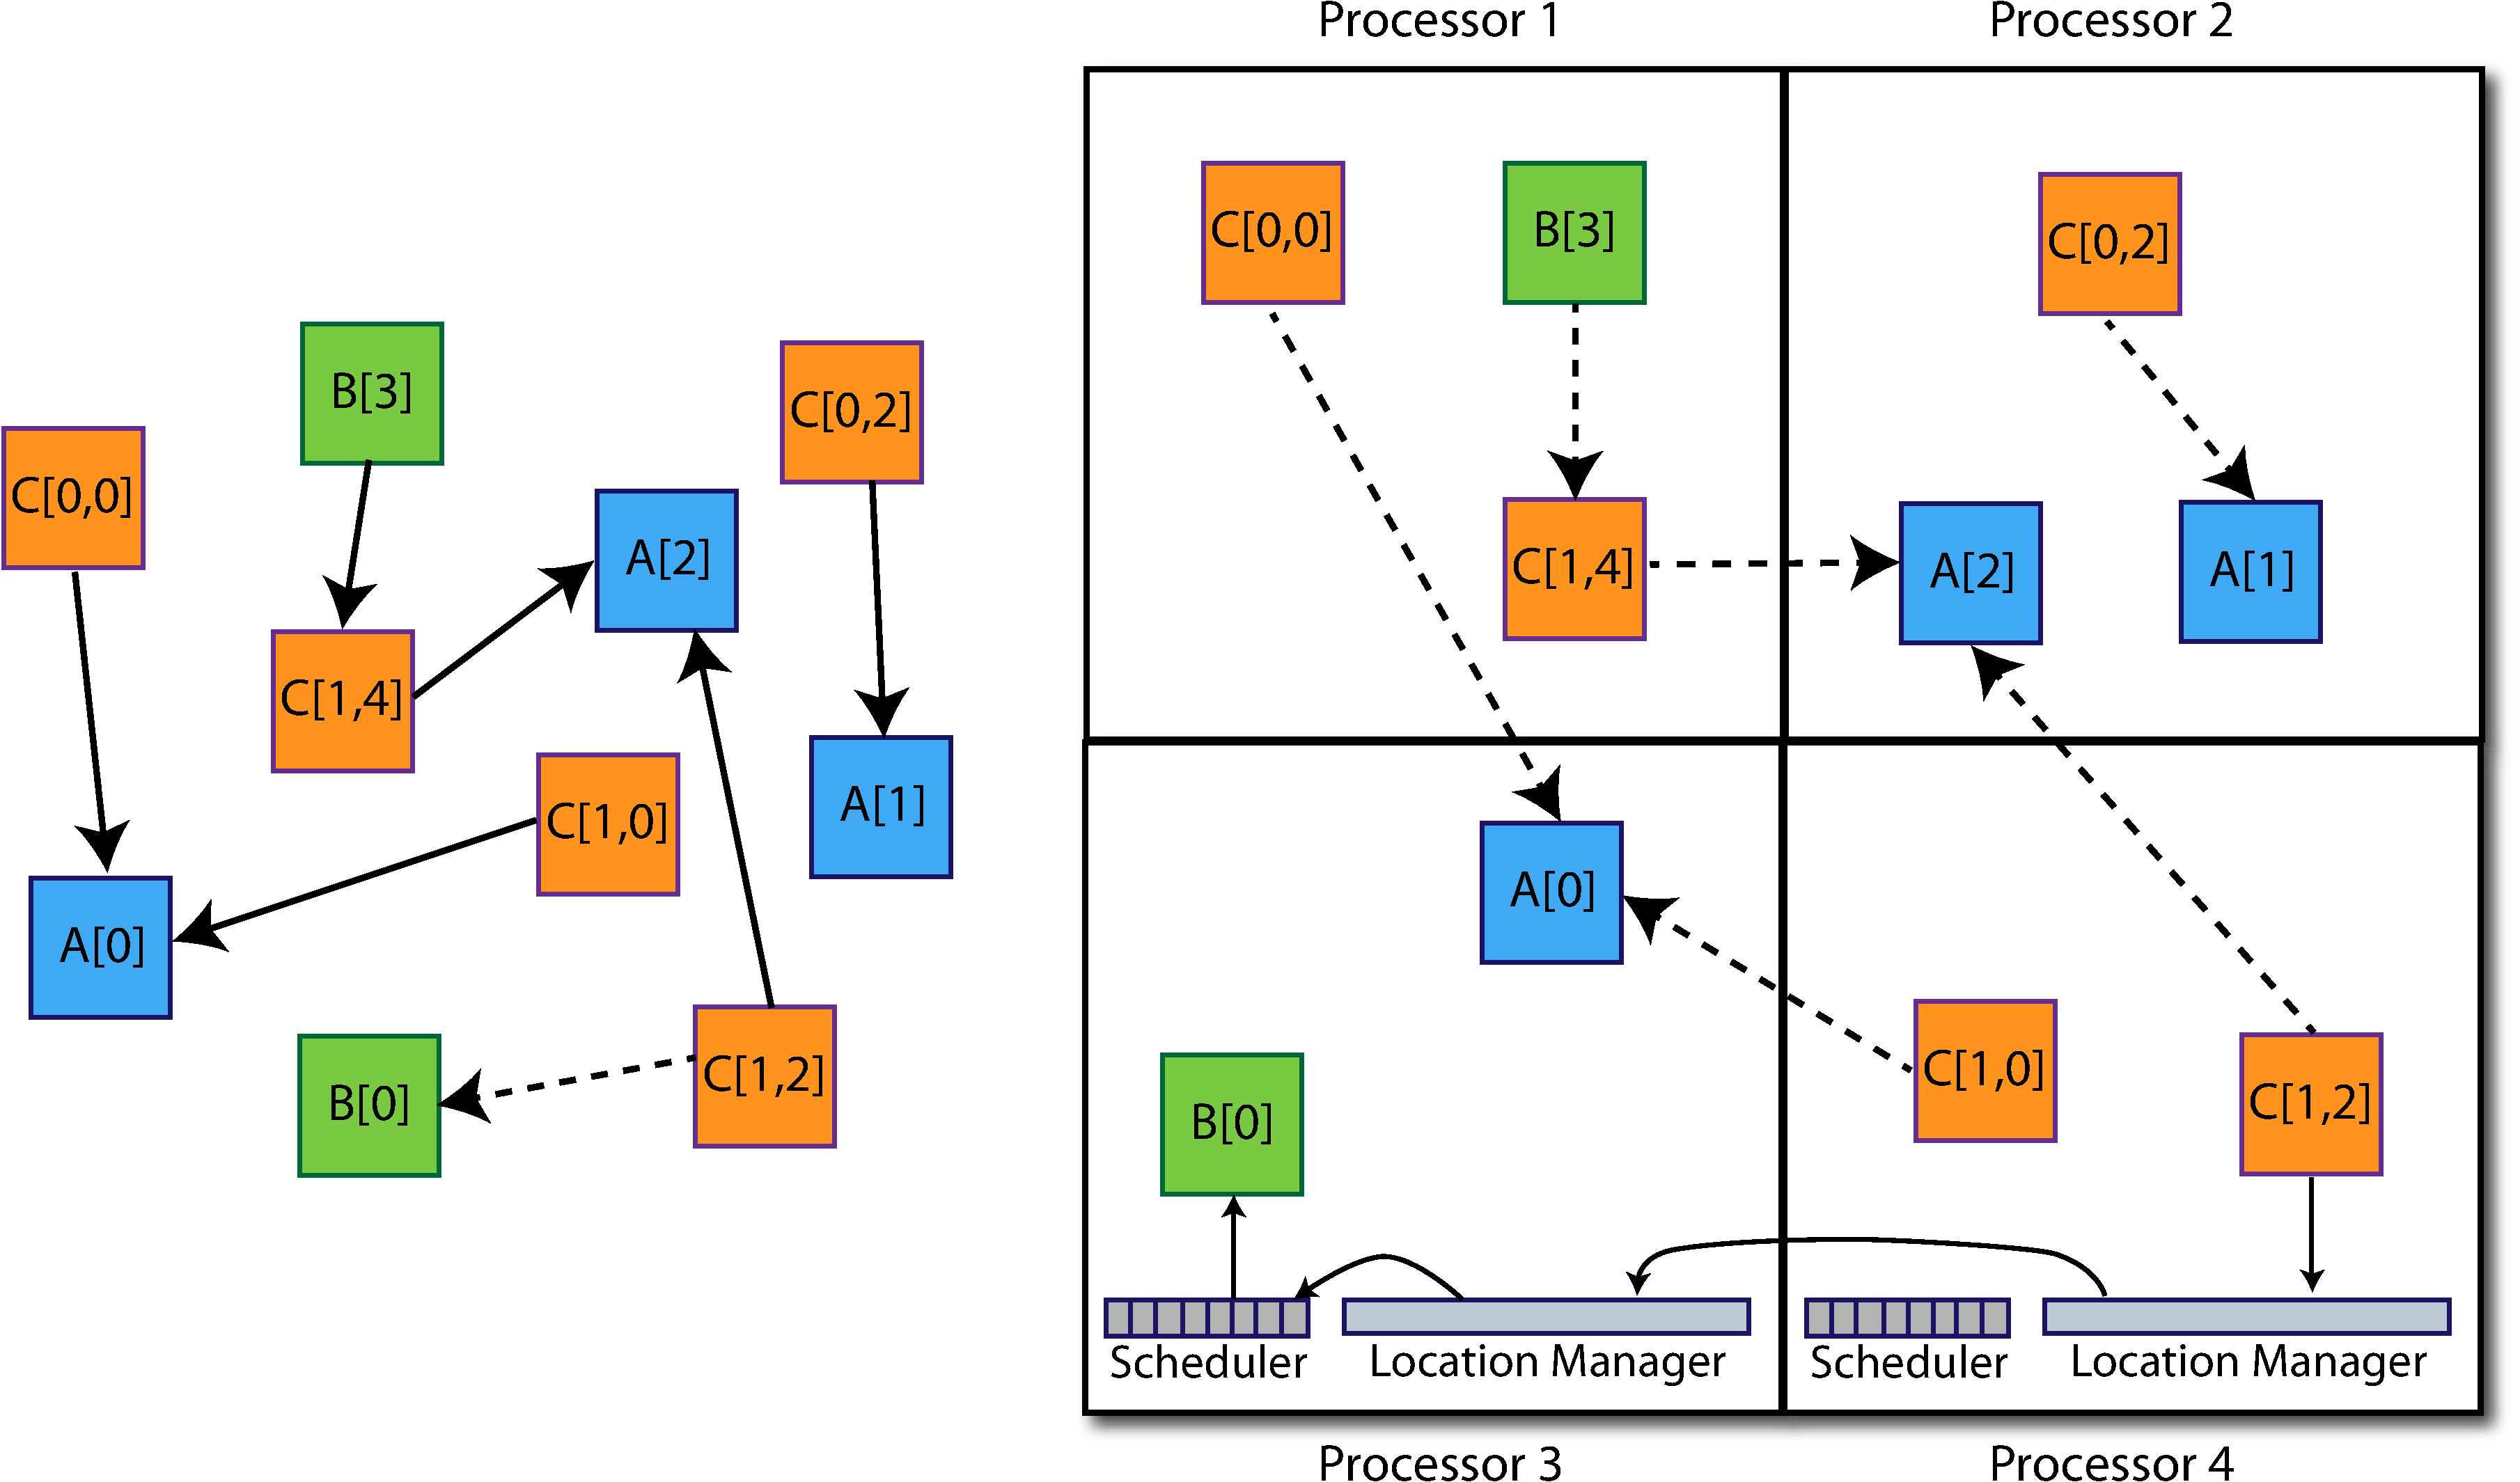
\includegraphics[width=0.9\textwidth]{figures/elements2.pdf}\end{center}
\end{frame}

\begin{frame}[fragile]
  \frametitle{Collective Communication Operations}
  \begin{itemize}
    \item Point-to-point operations involve only two objects
    \item Collective operations that involve a collection of objects
    \item Broadcast: calls a method in each object of the array
    \item Reduction: collects a contribution from each object of the array
    \item A spanning tree is used to send/receive data
  \end{itemize}
    \begin{center} 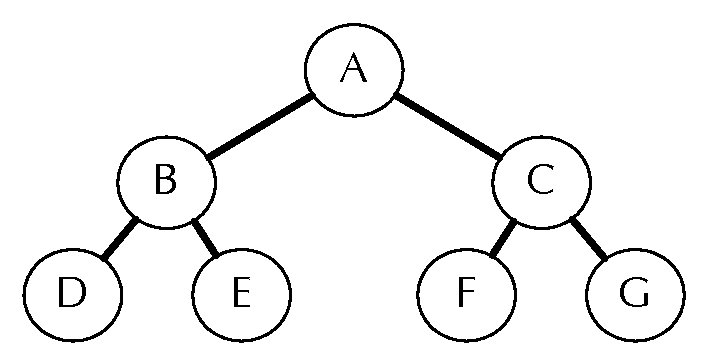
\includegraphics[width=0.5\textwidth]{figures/spanningTree.pdf} \end{center}
\end{frame}


\begin{frame}[fragile]
  \frametitle{Broadcast}
  \begin{itemize}
    \item A message to each object in a collection
    \item The chare array proxy object is used to perform a broadcast
    \item It looks like a function call to the proxy object
    \item From the main chare:
    \begin{lstlisting}
CProxy_Hello helloArray = CProxy_Hello::ckNew(helloArraySize);
helloArray.foo();
    \end{lstlisting}
    \item From a chare array element that is a member of the same array:
     \begin{lstlisting}
 thisProxy.foo()
    \end{lstlisting}
  \end{itemize}
\end{frame}

\begin{frame}[fragile]
  \frametitle{Reduction}
  \begin{itemize}
  \item Combines a set of values: sum, max, aggregate
  \item Usually reduces the set of values to a single value
  \item Combination of values requires an operator
  \item The operator must be commutative and associative
  \item Each object calls \code{contribute} in a reduction
  \end{itemize}
\end{frame}

\begin{frame}[fragile]
  \frametitle{Reduction: Example}
  \lstinputlisting{code/reductionMainTarget.ci}
\end{frame}

\begin{frame}[fragile]
  \frametitle{Reduction: Example}
  \lstinputlisting[basicstyle=\tiny]{code/reductionMainTarget.cpp}
Output:
  \begin{lstlisting}[basicstyle=\tiny]
value: 1176
Program finished.
  \end{lstlisting}
\end{frame}

\begin{frame}[fragile]
  \frametitle{Quick Hands-on}
  \begin{itemize}
  \item Log onto your vesta account.
  \item Obtain the following code:\\ git clone git://charm.cs.uiuc.edu/users/tutorial\_exercise
  \item Read the README.
  \item Change to toy directory, and read assignment.txt.
  \item Uncomment the CHARMC declaration at top of Makefile.
  \item ./charmrun -A $<$your\_account$>$ +p4 ./hello 16.
  \item Modify paramter to be an array instead of int.
  \end{itemize}
\end{frame}


\section[LB]{Using Dynamic Load Balancing}
\transition{The PUP Framework}
\begin{frame}[fragile]
\frametitle{Chare Migration: motivations}
\begin{itemize}
\item Chares are initially placed according to a placement map
\begin{itemize}
\item The user can specify this map
\end{itemize}
\item While running, some processors might be overloaded
\begin{itemize}
\item Need to rebalance the load
\end{itemize}
\item Automatic checkpoint
\begin{itemize}
\item Migration to disk
\end{itemize}
\item Chares are made serializable for transport using the Pack UnPack (PUP) framework
\end{itemize}
\end{frame}

\begin{frame}[fragile]
\frametitle{The PUP Process}
  \begin{center}
    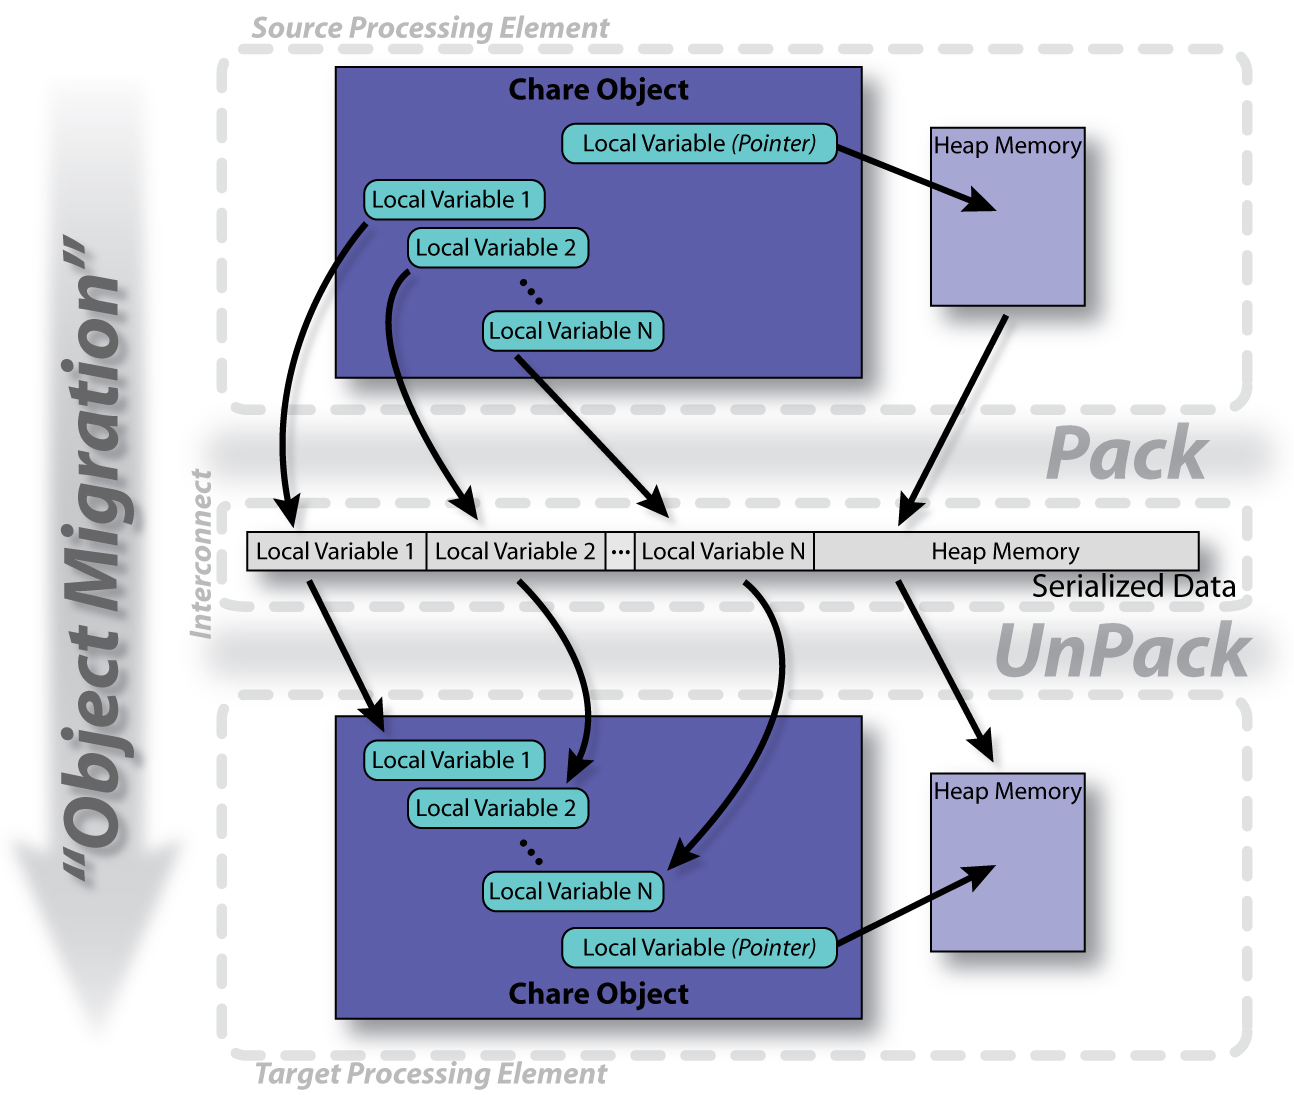
\includegraphics[width=0.8\textwidth]{figures/PUPProcess.png}
  \end{center}
\end{frame}


% \begin{frame}[fragile]
% \frametitle{PUP Usage Sequence}
%   \begin{center}
%     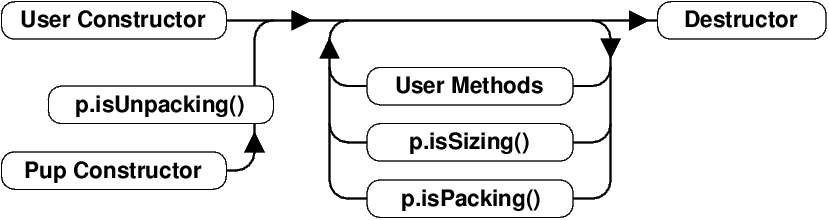
\includegraphics[width=0.8\textwidth]{figures/PUPUsage.png}
%   \end{center}
% \begin{columns}
%  \begin{column}{0.5\textwidth}
%  \begin{itemize}
%  \item Migration out:
%  \begin{itemize}
%  \item ckAboutToMigrate
%  \item Sizing
%  \item Packing
%  \item Destructor
%  \end{itemize}
%  \end{itemize}
%  \end{column}
%  \begin{column}{0.5\textwidth}
%  \begin{itemize}
%  \item Migration in:
%  \begin{itemize}
%  \item Migration constructor
%  \item UnPacking
%  \item ckJustMigrated
%  \end{itemize}
%  \end{itemize}
% \end{column}
% \end{columns}
% \end{frame}

\begin{frame}[fragile]
\frametitle{Writing a PUP routine}
 \begin{columns}
 \begin{column}{0.5\textwidth}
   \begin{lstlisting}
class MyChare : public CBase_MyChare {
  int a;   float b;   char c;
  float localArray[LOCAL_SIZE];
};
 \end{lstlisting}
 \end{column}
 \begin{column}{0.5\textwidth}
  \begin{lstlisting}
void pup(PUP::er &p) {
   CBase_MyChare::pup(p);
   p | a;  p | b; p | c;
}
  \end{lstlisting}
  \end{column}
  \end{columns}
\end{frame}

\begin{frame}[fragile]
\frametitle{Writing a PUP routine}
 \begin{columns}
 \begin{column}{0.5\textwidth}
   \begin{lstlisting}
class MyChare : public CBase_MyChare {
  int a;   float b;   char c;
  float localArray[LOCAL_SIZE];
  int heapArraySize;
  float* heapArray;
  MyClass *pointer;
 
  public:
   MyChare();
   MyChare(CkMigrateMessage *msg) {};
   ~MyChare() {
     if (heapArray != NULL) {
       delete [] heapArray;
       heapArray = NULL;
     }
};
 \end{lstlisting}
 \end{column}
 \begin{column}{0.5\textwidth}
  \begin{lstlisting}
void pup(PUP::er &p) {
   CBase_MyChare::pup(p);
   p | a;  p | b; p | c;
   p(localArray, LOCAL_SIZE);
   p | heapArraySize;
   if (p.isUnpacking()) {
     heapArray = new float[heapArraySize];
   }
   p(heapArray, heapArraySize);
   int isNull = (pointer==NULL) ? 1 : 0;
   p | isNull;
   if (!isNull) {
     if (p.isUnpacking()) pointer = new MyClass();
     p | *pointer;
   }
 }
}
  \end{lstlisting}
  \end{column}
  \end{columns}
\end{frame}


\begin{frame}[fragile]
\frametitle{PUP: Concerns}
\begin{itemize}
\item If variables are added to an object, update the PUP routine
\item If the object allocates data on the heap, copy it recursively, not just the pointer
\item Remember to allocate memory while unpacking
\item Sizing, Packing, and Unpacking must scan the variables in the same order
\item Test PUP routines with “+balancer RotateLB”
\end{itemize}
\end{frame}

\transition{Dynamic Load Balancing}

\begin{frame}[fragile]
\frametitle{How to Diagnose Load Imbalance}
\begin{itemize}
 \item Often hidden in statements such as:
 \begin{itemize}
  \item Very high synchronization overhead
  \begin{itemize}
   \item Most processors are waiting at a reduction
  \end{itemize}
 \end{itemize}
 \item Count total amount of computation (ops/flops) per processor
 \begin{itemize}
  \item In each phase! 
  \item Because the balance may change from phase to phase
 \end{itemize}
\end{itemize}
\end{frame}

\begin{frame}[fragile]
\frametitle{Golden Rule of Load Balancing}
\emph{Fallacy: objective of load balancing is to minimize variance in load across processors}

\begin{itemize}
 \item[]\emph{Example:}
 \begin{itemize}
  \item  50,000 tasks of equal size, 500  processors:
  \begin{itemize}
   \item A: All processors get 99, except last 5 gets $100+99 = 199$
   \item OR, B:  All processors have 101, except last 5 get 1
  \end{itemize}
 \end{itemize}
 \item[] Identical variance, but situation A is much worse!
\end{itemize}


\emph{Golden Rule: It is ok if a few processors idle, but avoid having processors that are overloaded with work}


\emph{Finish time} = $max_i$(Time on processor $i$)
\begin{itemize}
\item[] excepting data dependence and communication overhead issues
\end{itemize}

The speed of any group is the speed of slowest member of that group.
\end{frame}

\begin{frame}[fragile]
\frametitle{Automatic Dynamic Load Balancing}
\begin{itemize}
\item Measurement based load balancers
\begin{itemize}
\item Principle of persistence: In many CSE applications, computational loads and communication patterns tend to persist, even in dynamic computations
\item Therefore, recent past is a good predictor of near future
\item Charm++ provides a suite of load-balancers 
\item Periodic measurement and migration of objects
\end{itemize}
\item Seed balancers (for task-parallelism)
\begin{itemize}
\item Useful for divide-and-conquer and state-space-search applications
\item Seeds for charm++ objects moved around until they take root
\end{itemize}
\end{itemize}
\end{frame}

\begin{frame}[fragile]
\frametitle{Using the Load Balancer}
\begin{itemize}
\item link a LB module 
\begin{itemize}
\item \code{-module <strategy>}
\item RefineLB, NeighborLB, GreedyCommLB, others…
\item EveryLB will include all load balancing strategies
\end{itemize}
\item compile time option (specify default balancer)
\begin{itemize}
\item \code{-balancer RefineLB}
\item runtime option
\item \code {+balancer RefineLB}
\end{itemize}
\end{itemize}
\end{frame}

\begin{frame}
\frametitle{Code to Use Load Balancing}
\begin{itemize}
\item Insert \code{if (myLBStep) AtSync() else ResumeFromSync();} call at natural barrier
\item Implement \code{ResumeFromSync()} to resume execution
\begin{itemize}
\item Typical ResumeFromSync contribute to a reduction
\end{itemize}
\end{itemize}
\end{frame}

\begin{frame}[fragile]
\frametitle{Example: Stencil}
\begin{lstlisting}[basicstyle=\tiny]
while (!converged) {
  serial {
    int x = thisIndex.x, y = thisIndex.y, z = thisIndex.z;
    copyToBoundaries();
    thisProxy(wrapX(x-1),y,z).updateGhosts(i, RIGHT, dimY, dimZ, right);
    /* ...similar calls to send the 6 boundaries... */
    thisProxy(x,y,wrapZ(z+1)).updateGhosts(i, FRONT, dimX, dimY, front);
  }
  for (remoteCount = 0; remoteCount < 6; remoteCount++) {
    when updateGhosts[i](int i, int d, int w, int h, double b[w*h])
    serial { updateBoundary(d, w, h, b); }
  }
  serial {
    int c = computeKernel() < DELTA;
    CkCallback cb(CkReductionTarget(Jacobi, checkConverged), thisProxy);
    if (i%5 == 1) contribute(sizeof(int), \&c, CkReduction::logical_and, cb);
  }
  if (i % lbPeriod == 0) { serial { AtSync(); } when ResumeFromSync() {} }
  if (++i % 5 == 0) {
    when checkConverged(bool result) serial {
      if (result) { mainProxy.done(); converged = true; }
    }
  }
}
\end{lstlisting}
\end{frame}

\begin{frame}
\frametitle{Performance}
\begin{centering}
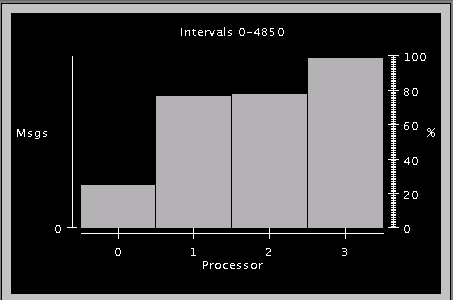
\includegraphics[width=0.5\textwidth]{figures/beforeLB}
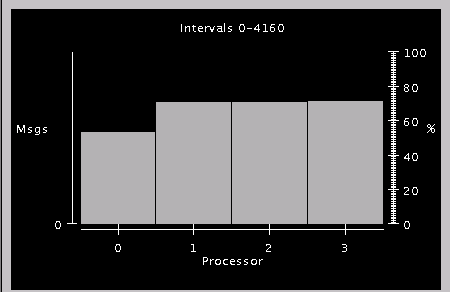
\includegraphics[width=0.5\textwidth]{figures/afterLB}
\end{centering}
\end{frame}

%\begin{frame}[fragile]
%\frametitle{Grainsize and Load Balancing}
%\begin{itemize}
%\item[] How Much Balance Is Possible?
%\end{itemize}
%\begin{columns}
%  \begin{column}[T]{2.8in}
%  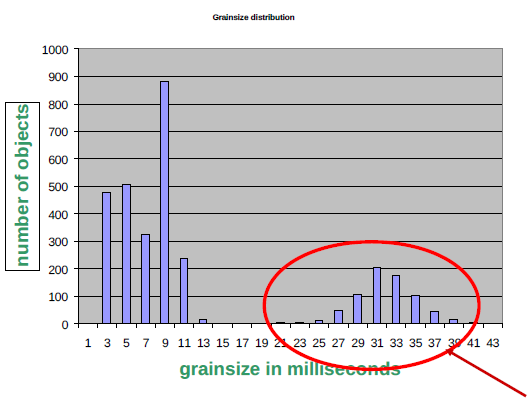
\includegraphics[width=2.8in, height=2.0in]{figures/histogramGrains}
%  \end{column}
%
%  \begin{column}[T]{5cm}
%  Solution:\\ 
%  Split compute objects that may have too much work,
%  using a heuristic based on number of interacting atoms
%  \end{column}
%\end{columns}
%\end{frame}

%\begin{frame}[fragile]
%\frametitle{Grainsize For Extreme Scaling}
%\begin{itemize}
% \item Strong Scaling is limited by expressed parallelism
% \begin{itemize}
%  \item Minimum iteration time limited by lengthiest computation
%  \begin {itemize} 
%    \item Largest grains set lower bound
%  \end{itemize}
% \end{itemize}
% \item 1-away generalized to k-away provides fine granularity control
%\end{itemize}
%\begin{centering}
%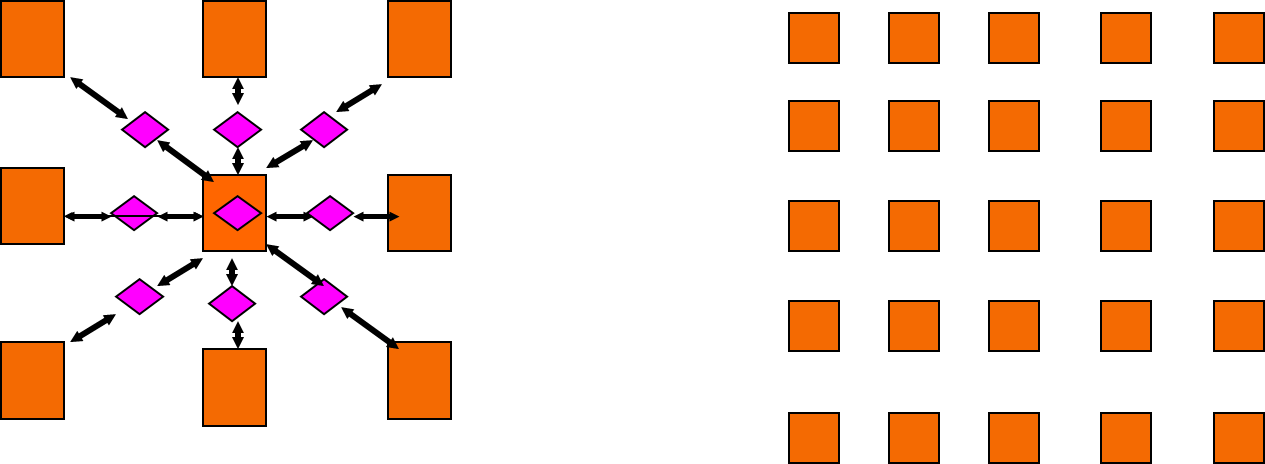
\includegraphics[width=1.0\textwidth]{figures/1away2away}
%\end{centering}
%\end{frame}
%
%\begin{frame}[fragile]
%\frametitle{NAMD: 2-AwayX Example}
%\begin{centering}
%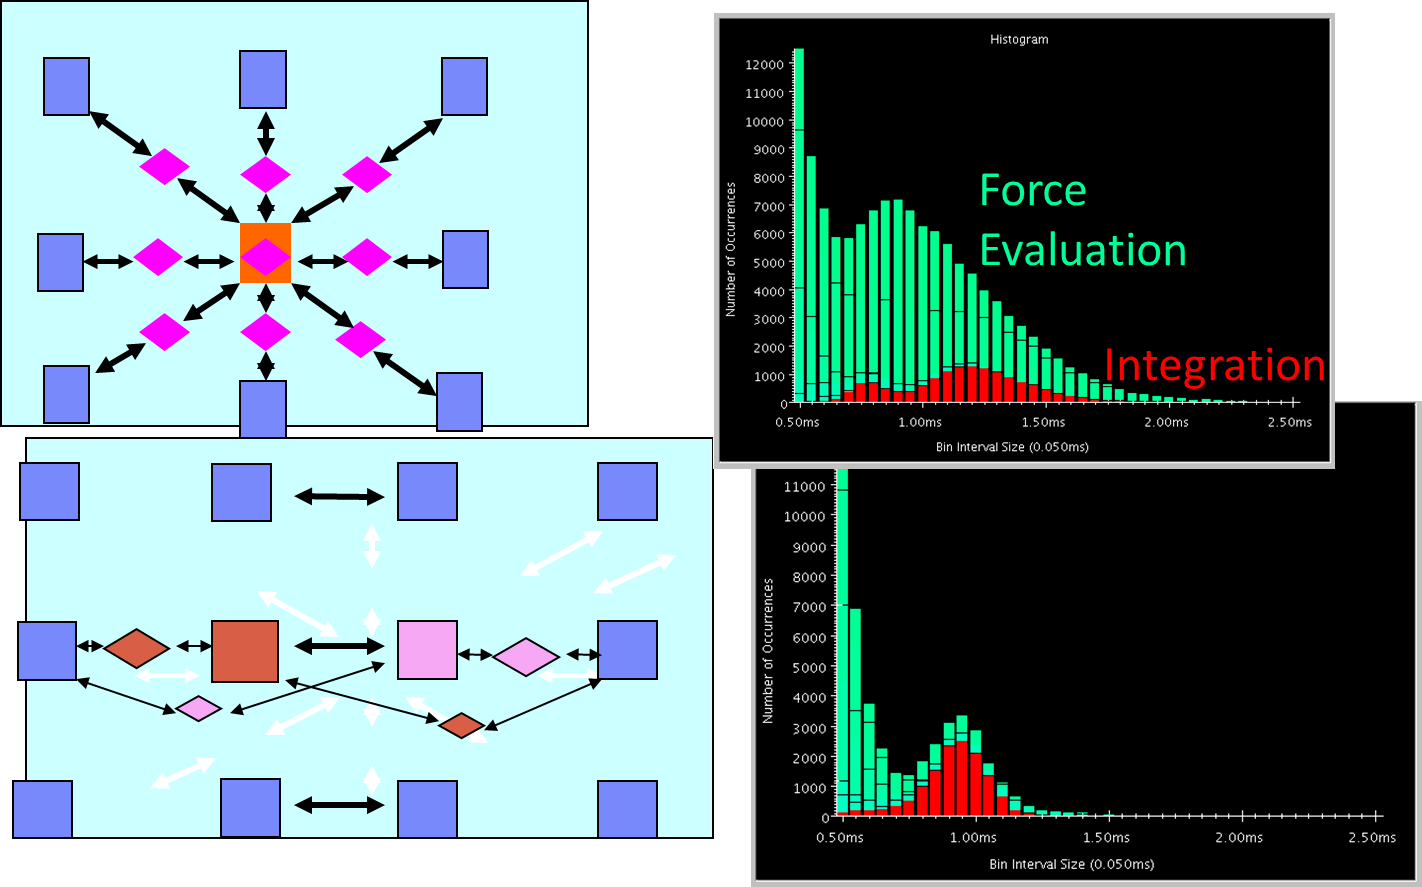
\includegraphics[width=1.0\textwidth]{figures/2awayDiagramPlusHistos}
%\end{centering}
%\end{frame}
%
\begin{frame}[fragile]
\frametitle{Load Balancing Strategies}
\begin{itemize}
 \item Classified by when it is done:
 \begin{itemize}
  \item Initially
  \item Dynamic: Periodically
  \item Dynamic: Continuously
 \end{itemize}
 \item Classified by whether decisions are taken with global information
 \begin{itemize}
  \item Fully centralized
  \begin{itemize}
   \item Quite good a choice when load balancing period is high
  \end{itemize}
 \item Fully distributed
 \begin{itemize}
  \item Each processor knows only about a constant number of neighbors
  \item Extreme case: totally local decision (send work to a random destination processor, with some probability).
 \end{itemize}
\item Use \emph{aggregated} global  information, and \emph{detailed} neighborhood info.
\end{itemize}
\end{itemize}
\end{frame}

\begin{frame}[fragile]
\frametitle{Dynamic Load Balancing Scenarios}
\begin{itemize}
 \item Examples representing typical classes of situations
 \begin{itemize}
  \item Particles distributed over simulation space
  \begin{itemize}
   \item Dynamic: because Particles move.
   \item Cases:\\
   Highly non-uniform distribution (cosmology)\\
   Relatively Uniform distribution 
   %\begin{description}[parskip]
   %\item Highly non-uniform distribution (cosmology)
   %\item Relatively Uniform distribution 
   %\end{description}
  \end{itemize}
 \end{itemize}
\item Structured grids, with dynamic refinements/coarsening
\item Unstructured grids with dynamic refinements/coarsening
\end{itemize}
\end{frame}

%\begin{frame}[fragile]
%\frametitle{Example Case: Particles}
% Orthogonal Recursive Bisection (ORB)
% %should wrapfig the little diagram here
% \begin{itemize} 
%  \item At each stage: divide Particles equally
%  \item Processor don’t need to be a power of 2:
%  \begin{itemize} 
%   \item Divide in proportion 
%   \begin{itemize} 
%    \item 2:3 with 5 processors
%   \end{itemize}
%  \end{itemize}
% \item How to choose the dimension along which to cut?
% \begin{itemize} 
%  \item Choose the longest one
% \end{itemize}
% \item How to draw the line?
% \begin{itemize} 
%  \item All data on one processor? Sort along each dimension
%  \item Otherwise: run a distributed histogramming algorithm to find the line, recursively
% \end{itemize}
% \item Find the entire tree, and then do all data movement at once
% \begin{itemize} 
%  \item Or do it in two-three steps.
%  \item But no reason to redistribute particles after drawing each line.
% \end{itemize}
%\end{itemize}
%\end{frame}

\begin{frame}[fragile]
\frametitle{Dynamic Load Balancing using Objects}

Object based decomposition (I.e. virtualized decomposition) helps
\begin{itemize}
 \item Allows RTS to remap them to balance load
 \item But how does the RTS decide where to map objects?
 \item Just move objects away from overloaded processors to underloaded processors
 \item How is load determined?
\end{itemize}
\end{frame}

\begin{frame}[fragile]
\frametitle{Measurement Based Load Balancing}
\begin{itemize}
 \item \emph{Principle of Persistence}
 \begin{itemize}
  \item Object communication patterns and computational loads tend to persist over time
  \item In spite of dynamic behavior
  \begin{itemize}
   \item Abrupt but infrequent changes
   \item Slow and small changes
  \end{itemize}
 \end{itemize}
\item Runtime instrumentation
\begin{itemize}
 \item Measures communication volume and computation time
\end{itemize}
\item Measurement based load balancers
\begin{itemize}
 \item Use the instrumented data-base periodically to make new decisions
 \item Many alternative strategies can use the database
\end{itemize}
\end{itemize}
\end{frame}

\begin{frame}[fragile]
\frametitle{Periodic Load Balancing}

Centralized strategies:
\begin{itemize}
 \item Charm RTS collects data (on one processor) about:
 \begin{itemize}
  \item Computational Load and Communication for each pair
 \end{itemize}
 %\item If you are not using AMPI/Charm, you can do the same instrumentation and data collection
 \item Partition the graph of objects across processors
 \begin{itemize}
  \item Take communication into account
  \begin{itemize}
   \item Pt-to-pt, as well as multicast over a subset
   \item As you map an object, add to the load on both sending and receiving processor
  \end{itemize}
  \item Multicasts to multiple co-located objects are effectively the cost of a single send
 \end{itemize}
\end{itemize}
\end{frame}

\begin{frame}[fragile]
\frametitle{Typical Load Balancing Steps}
\begin{centering}
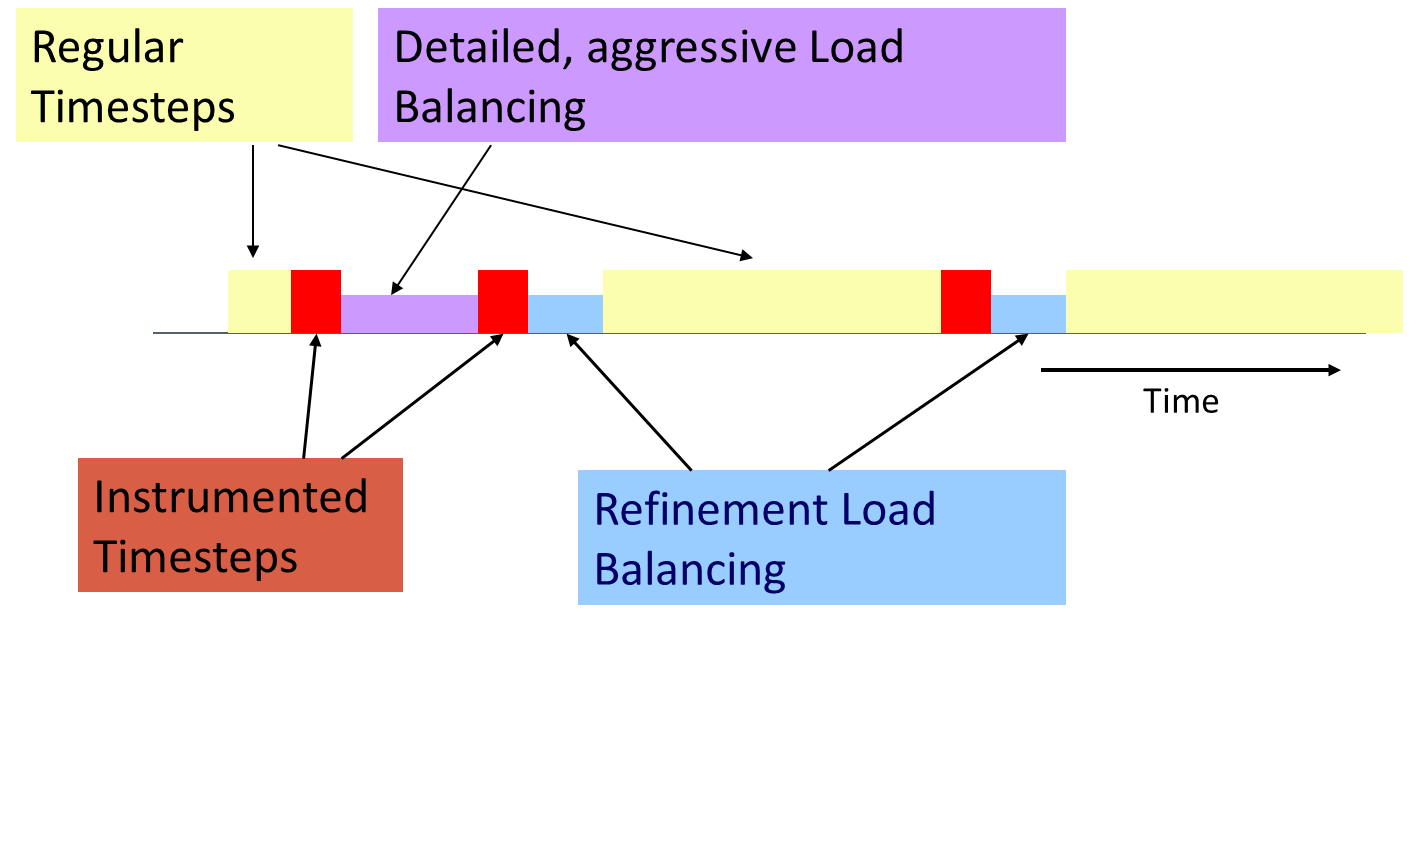
\includegraphics[width=1.0\textwidth]{figures/LBStepsDiagram}
\end{centering}
\end{frame}

% \begin{frame}[fragile]
% \frametitle{Object Partitioning Strategies}
% \begin{itemize}
%  \item You can use graph partitioners like METIS, K-R
%  \begin{itemize}
%   \item BUT: graphs are smaller, and optimization criteria are different
%  \end{itemize}
%  \item Greedy strategies:
%  \begin{itemize}
%   \item If communication costs are low: use a simple greedy strategy
%   \begin{itemize}
%    \item Sort objects by decreasing load
%    \item Maintain processors in a heap (by assigned load)
%    \item In each step: \\
%    %\begin{description}
%    % \item 
%    assign the heaviest remaining object to the least loaded processor
%    %\end{description}
%   \end{itemize}
%   \item With small-to-moderate communication cost:
%   \begin{itemize}
%    \item Same strategy, but add communication costs as you add an object to a processor
%   \end{itemize}
%   \item Always add a refinement step at the end:
%   \begin{itemize}
%    \item Swap work from heaviest loaded processor to ``some other processor''
%    \item Repeat a few times or until no improvement 
%   \end{itemize}
%  \end{itemize}
% \end{itemize}
% \end{frame}


% \begin{frame}[fragile]
% \frametitle{Object Partitioning Strategies 2}
% When communication cost is significant:
% \begin{itemize}
%  \item Still use greedy strategy, but:
%  \begin{itemize}
%   \item At each assignment step, choose between assigning O to least loaded processor and the processor that already has objects that communicate most with O.
%   \begin{itemize}
%    \item Based on the degree of difference in the two metrics
%    \item Two-stage assignments:\\
%     In early stages,  consider communication costs as long as the processors are
%     in the same (broad) load “class”,\\
%     In later stages, decide based on load
%   \end{itemize}
%  \end{itemize}
% \end{itemize}
% Branch-and-bound
% \begin{itemize}
%  \item Searches for optimal, but can be stopped after a fixed time
% \end{itemize}
% \end{frame}

\begin{frame}[fragile]
\frametitle{Crack Propagation}
\begin{centering}
\includegraphics[width=0.4\textwidth]{figures/chunkGraph16}
\includegraphics[width=0.4\textwidth]{figures/chunkGraph128}
\end{centering}
Decomposition into 16 chunks (left) and 128 chunks, 8 for each PE (right). The middle area contains cohesive elements. Both decompositions obtained using Metis. Pictures: S. Breitenfeld, and P. Geubelle

As computation progresses, crack propagates, and new elements are added, leading to more complex computations in some chunks
\end{frame}

\begin{frame}[fragile]
\frametitle{Load Balancing Crack Propagation}
\begin{centering}
\includegraphics[width=1.0\textwidth]{figures/LButilizationCrackPropWithAnnotation}
\end{centering}
\end{frame}


\begin{frame}[fragile]
\frametitle{Distributed Load balancing}
\begin{itemize}
 \item Centralized strategies
 \begin{itemize}
  \item Still ok for 3000 processors for NAMD
 \end{itemize}
 \item Distributed balancing is needed when:
 \begin{itemize}
  \item Number of processors is large and/or 
  \item load variation is rapid
 \end{itemize}
 \item Large machines: 
 \begin{itemize}
  \item Need to handle locality of communication
  \begin{itemize}
   \item Topology sensitive placement
  \end{itemize}
  \item Need to work with scant global information
  \begin{itemize}
   \item Approximate or aggregated global information (average/max load)
   \item Incomplete global info (only “neighborhood”)
   \item Work diffusion strategies (1980s work by Kale and others!)
  \end{itemize}
  \item Achieving global effects by local action…
 \end{itemize}
\end{itemize}
\end{frame}

\begin{frame}[fragile]
\frametitle{Load Balancing on Large Machines}
\begin{itemize}
 \item Centralized load balancing strategies don’t scale on extremely large machines
 \item Limitations of centralized strategies:
 \begin{itemize}
  \item Central node: memory/communication bottleneck
  \item Decision-making algorithms tend to be very slow
 \end{itemize}
 \item Limitations of distributed strategies:
 \begin{itemize}
  \item Difficult to achieve well-informed load balancing decisions
 \end{itemize}
\end{itemize}
\end{frame}


\begin{frame}[fragile]
\frametitle{Simulation Study - Memory Overhead}
lb\_test experiments performed with the performance simulator BigSim
\includegraphics[width=1.0\textwidth]{figures/LBMemOverhead}
\begin{itemize}
 \item lb\_test benchmark is a parameterized program that creates a 
specified number of communicating objects in 2D-mesh.
\end{itemize}
\end{frame}


\begin{frame}[fragile]
\frametitle{Hierarchical Load Balancers}
\begin{itemize}
\item Partition processor allocation into processor groups
\item Apply different strategies at each level
\item Scalable to a large number of processors
\end{itemize}
\end{frame}

\begin{frame}[fragile]
\frametitle{Our Hybrid Scheme}
\includegraphics[width=1.0\textwidth]{figures/hybridLBScheme}
\end{frame}

\begin{frame}[fragile]
\frametitle{Hybrid Load Balancing Performance}
\includegraphics[width=0.5\textwidth]{figures/hybridLBPerf}
\includegraphics[width=0.5\textwidth]{figures/hybridLBquality}
\end{frame}

\begin{frame}[fragile]
\frametitle{MetaBalancer - When and how to load balance?}
\begin{itemize}    
    \item Difficult to find the optimum load balancing period
    \begin{itemize}
       \item Depends on the application characteristics
       \item Depends on the machine the application is run on
    \end{itemize}
    
    \item Monitors the application continuously and predicts behavior.
    \item Decides when to invoke which load balancer.
    \item Command line argument - \texttt{+MetaLB}
\end{itemize}
\end{frame}

\begin{frame}[fragile]
\frametitle{Metabalancer Performance for LeanMD mini-App}
\includegraphics{figures/bgp-metabalancer-leanmd}
\end{frame}

\section[ChaNGa]{Compiling and Using Charm++ with ChaNGa}
\begin{frame}
  \frametitle{Installing Charm}
  \begin{itemize}
    \item Downloading Charm
    \begin{itemize}
      \item \texttt{git clone git://charm.cs.illinois.edu/charm.git}
    \end{itemize}
    \item Building Charm
    \begin{itemize}
      \item \texttt{./build <TARGET> <TARGET ARCHITECTURE> [OPTIONS]}
      \item Net with 64 bit Linux 
      \begin{itemize}
        \item \texttt{./build charm++ net-linux-x86\_64}
      \end{itemize}
      \item Net with 64 bit Linux shared memory (SMP)
      \begin{itemize}
        \item \texttt{./build charm++ net-linux-x86\_64 smp}
      \end{itemize}
      \item Optimized build
      \begin{itemize}
        \item \texttt{./build charm++ net-linux-x86\_64 -with-production}
      \end{itemize}
      \item Ibverbs with 64 bit Linux 
      \begin{itemize}
        \item \texttt{./build charm++ net-linux-x86\_64 ibverbs}
      \end{itemize}
      \item MPI with 64 bit Linux
      \begin{itemize}
        \item \texttt{./build charm++ mpi-linux-x86\_64}
      \end{itemize}
    \end{itemize}
  \end{itemize}
\end{frame}

\begin{frame}
  \frametitle{Compiling a Charm++ Program}
  \begin{center}
    \includegraphics[width=0.9\textwidth]{figures/charmCompile.jpg}
  \end{center}
  \begin{itemize}
    \item Compiling Hello World Example
    \begin{itemize}
      \item \texttt{charmc hello.ci}
      \item \texttt{charmc -c hello.cpp}
      \item \texttt{charmc -o hello hello.o}
    \end{itemize}
  \end{itemize}
\end{frame}

\begin{frame}
  \frametitle{Running a Charm++ Program}
  \begin{itemize}
    \item Run commands
    \begin{itemize}
      \item \texttt{./charmrun +p7 ./pgm}
      \item The \texttt{+p7} tells the system to use seven cores
    \end{itemize}
    \item In debug mode
    \begin{itemize}
      \item Compile with \texttt{-g} option
      \item \texttt{./charmrun +p7 ./pgm ++debug}
      \item Runs each node under gdb in an xterm window
    \end{itemize}
    \item In SMP mode
    \begin{itemize}
      \item \texttt{./charmrun +p14 ./pgm +ppn 7 +pemap 1-7 +commap 0}
      \item \texttt{+ppn} tells the number of pes per node
      \item \texttt{+pemap} binds execution threads to sequence of cores
      \item \texttt{+commap} binds communication threads to the listed cores
    \end{itemize}
  \end{itemize}
\end{frame}


\begin{frame}
  \frametitle{Running ChaNGa}
  \begin{itemize}
    \item Compile
    \begin{itemize}
      \item \texttt{git clone git://charm.cs.illinois.edu/cosmo/changa.git}
      \item \texttt{git clone git://charm.cs.illinois.edu/cosmo/utility.git}
      \item \texttt{cd changa}
      \item \texttt{./configure CHARM\_DIR=<path\_to\_charm>}
      \item \texttt{make -j4}
    \end{itemize}
    \item Run
    \begin{itemize}
      \item \texttt{Download the dataset}
      \item \texttt{./charmrun +p1024 ./ChaNGa -D 1 -ppc 125 -p 52000 -killat 2 ./dwf1.2048.param
      +balancer Orb3dLB\_notopo +LBPeriod 0.1 +LBCommOff +noAnytimeMigration}
    \end{itemize}
  \end{itemize}
\end{frame}


\section[Tuning]{Performance Tuning}
\begin{frame}
  \frametitle{Performance Analysis Using Projections}
  \begin{itemize}
  \item Instrumentation and measurement
  \begin{itemize}
  \item Link program with {\tt -tracemode projections or summary}
  \item Trace data is generated automatically during run
  \item User events can be easily inserted as needed
  \end{itemize}
  \item Projections: visualization and analysis
  \begin{itemize}
  \item Scalable tool to analyze up to 200,000 log files
  \item A rich set of tool features : time profile, time lines, usage profile, histogram, extrema tool
  \item Detect performance problems: load imbalance, grainsize, communication bottleneck, etc 
  \end{itemize}
  \end{itemize}

\end{frame}

\begin{frame}[fragile]
\frametitle{Conclusion}
\begin{itemize}
  \item Charm++ is a production-ready parallel programming system
  \item Program mostly in C++
  \item Very powerful runtime system
    \begin{itemize}
    \item Dynamic load balancing
    \item Automatic overlap of computation and communication
    \item Fault tolerance built in
    \end{itemize}
  \item Topics we did not cover:
    \begin{itemize}
    \item Many different types of load balancers
    \item Threaded methods in detail
    \item Futures
    \item Accelerator support
    \item Topology aware communication strategies
    \end{itemize}
  \item More information on \texttt{http://charm.cs.illinois.edu/}
\end{itemize}
\end{frame}
 


\end{document}



